\documentclass[twoside]{book}

% Packages required by doxygen
\usepackage{fixltx2e}
\usepackage{calc}
\usepackage{doxygen}
\usepackage[export]{adjustbox} % also loads graphicx
\usepackage{graphicx}
\usepackage[utf8]{inputenc}
\usepackage{makeidx}
\usepackage{multicol}
\usepackage{multirow}
\PassOptionsToPackage{warn}{textcomp}
\usepackage{textcomp}
\usepackage[nointegrals]{wasysym}
\usepackage[table]{xcolor}

% Font selection
\usepackage[T1]{fontenc}
\usepackage[scaled=.90]{helvet}
\usepackage{courier}
\usepackage{amssymb}
\usepackage{sectsty}
\renewcommand{\familydefault}{\sfdefault}
\allsectionsfont{%
  \fontseries{bc}\selectfont%
  \color{darkgray}%
}
\renewcommand{\DoxyLabelFont}{%
  \fontseries{bc}\selectfont%
  \color{darkgray}%
}
\newcommand{\+}{\discretionary{\mbox{\scriptsize$\hookleftarrow$}}{}{}}

% Page & text layout
\usepackage{geometry}
\geometry{%
  a4paper,%
  top=2.5cm,%
  bottom=2.5cm,%
  left=2.5cm,%
  right=2.5cm%
}
\tolerance=750
\hfuzz=15pt
\hbadness=750
\setlength{\emergencystretch}{15pt}
\setlength{\parindent}{0cm}
\setlength{\parskip}{3ex plus 2ex minus 2ex}
\makeatletter
\renewcommand{\paragraph}{%
  \@startsection{paragraph}{4}{0ex}{-1.0ex}{1.0ex}{%
    \normalfont\normalsize\bfseries\SS@parafont%
  }%
}
\renewcommand{\subparagraph}{%
  \@startsection{subparagraph}{5}{0ex}{-1.0ex}{1.0ex}{%
    \normalfont\normalsize\bfseries\SS@subparafont%
  }%
}
\makeatother

% Headers & footers
\usepackage{fancyhdr}
\pagestyle{fancyplain}
\fancyhead[LE]{\fancyplain{}{\bfseries\thepage}}
\fancyhead[CE]{\fancyplain{}{}}
\fancyhead[RE]{\fancyplain{}{\bfseries\leftmark}}
\fancyhead[LO]{\fancyplain{}{\bfseries\rightmark}}
\fancyhead[CO]{\fancyplain{}{}}
\fancyhead[RO]{\fancyplain{}{\bfseries\thepage}}
\fancyfoot[LE]{\fancyplain{}{}}
\fancyfoot[CE]{\fancyplain{}{}}
\fancyfoot[RE]{\fancyplain{}{\bfseries\scriptsize Generated by Doxygen }}
\fancyfoot[LO]{\fancyplain{}{\bfseries\scriptsize Generated by Doxygen }}
\fancyfoot[CO]{\fancyplain{}{}}
\fancyfoot[RO]{\fancyplain{}{}}
\renewcommand{\footrulewidth}{0.4pt}
\renewcommand{\chaptermark}[1]{%
  \markboth{#1}{}%
}
\renewcommand{\sectionmark}[1]{%
  \markright{\thesection\ #1}%
}

% Indices & bibliography
\usepackage{natbib}
\usepackage[titles]{tocloft}
\setcounter{tocdepth}{3}
\setcounter{secnumdepth}{5}
\makeindex

% Hyperlinks (required, but should be loaded last)
\usepackage{ifpdf}
\ifpdf
  \usepackage[pdftex,pagebackref=true]{hyperref}
\else
  \usepackage[ps2pdf,pagebackref=true]{hyperref}
\fi
\hypersetup{%
  colorlinks=true,%
  linkcolor=blue,%
  citecolor=blue,%
  unicode%
}

% Custom commands
\newcommand{\clearemptydoublepage}{%
  \newpage{\pagestyle{empty}\cleardoublepage}%
}

\usepackage{caption}
\captionsetup{labelsep=space,justification=centering,font={bf},singlelinecheck=off,skip=4pt,position=top}

%===== C O N T E N T S =====

\begin{document}

% Titlepage & ToC
\hypersetup{pageanchor=false,
             bookmarksnumbered=true,
             pdfencoding=unicode
            }
\pagenumbering{roman}
\begin{titlepage}
\vspace*{7cm}
\begin{center}%
{\Large Ray Tracer }\\
\vspace*{1cm}
{\large Generated by Doxygen 1.8.11}\\
\end{center}
\end{titlepage}
\clearemptydoublepage
\tableofcontents
\clearemptydoublepage
\pagenumbering{arabic}
\hypersetup{pageanchor=true}

%--- Begin generated contents ---
\chapter{Ray Tracer}
\label{index}\hypertarget{index}{}We are using a couple of C++11 features, so please ensure that you use an up-\/to-\/date compiler (G\+CC 4.\+7 or higher, Visual Studio 2012). \href{www.cmake.org}{\tt C\+Make} is used for setting up build environments.

\subsection*{Building under Linux/mac\+OS }

Inside the exercise\textquotesingle{}s top-\/level directory, execute the following commands\+: \begin{DoxyVerb}mkdir build
cd build
cmake ..
make
\end{DoxyVerb}


The last command -- i.\+e. {\ttfamily make} -- compiles the application. Rerun it whenever you have added/changed code in order to recompile.

To build a pretty documentation use\+: \begin{DoxyVerb}make doc
\end{DoxyVerb}


and open the {\ttfamily index.\+html} in the html folder with your favourite browser. To build the documentation, you must install Doxygen.

\subsection*{Building with X\+Code (mac\+OS) }

If you wish, you can use the C\+Make build system to generate an X\+Code project. Inside the exercise\textquotesingle{}s top-\/level directory, execute the following commands\+: \begin{DoxyVerb}mkdir xcode
cd xcode
cmake -G Xcode ..
open RayTracing.xcodeproj
\end{DoxyVerb}


\subsection*{Building under Microsoft Windows (Visual Studio) }


\begin{DoxyItemize}
\item Start the C\+Make-\/\+G\+UI.
\item Open the Ray\+Tracing top-\/level directory as source directory.
\item Choose a build directory.
\item Click on configure and select Visual Studio as generator.
\item Click generate to create the Visual Studio project files.
\item Open the Visual Studio solution file that is in the build directory you chose in C\+Make.
\end{DoxyItemize}

\subsection*{Running the \hyperlink{classRay}{Ray} Tracer }

The program expects two command line arguments\+: an input scene ({\ttfamily $\ast$.sce}) and an output image ({\ttfamily $\ast$.tga}). To render the scene with the three spheres, while inside the {\ttfamily build} directory, type\+: \begin{DoxyVerb}./raytrace ../scenes/spheres/spheres.sce output.tga
\end{DoxyVerb}


If you have finished all exercise tasks, use \begin{DoxyVerb}./raytrace 0
\end{DoxyVerb}


to render all scenes at once.

To set the command line parameters in M\+S\+VC or Xcode, please refer to the documentation of these programs (or use the command line...).

\subsection*{Assignment 1\+: Planes and Cylinders }

In this assignment, you will implement ray intersections with planes and cylinders and compute surface normals at the intersection points. The framework code provided this week is identical to last week\textquotesingle{}s, except {\ttfamily todo} comments have been inserted in {\ttfamily \hyperlink{Plane_8cpp}{Plane.\+cpp}} and `\+Cylinder to indicate where you need to add your implementations.

If you already set up a Git\+Hub repository last week to collaborate with your fellow group members, you can copy these T\+O\+DO comments over to your repository (or just note where your implementation needs to go and get started).

Please see the assignment handout P\+DF for more information and submission instructions. Note\+: there is a theory exercise for this assignment! 
\chapter{Hierarchical Index}
\section{Class Hierarchy}
This inheritance list is sorted roughly, but not completely, alphabetically\+:\begin{DoxyCompactList}
\item \contentsline{section}{Billboard}{\pageref{classBillboard}}{}
\item \contentsline{section}{Frame}{\pageref{structFrame}}{}
\item \contentsline{section}{G\+L\+F\+W\+\_\+window}{\pageref{classGLFW__window}}{}
\begin{DoxyCompactList}
\item \contentsline{section}{Solar\+\_\+viewer}{\pageref{classSolar__viewer}}{}
\end{DoxyCompactList}
\item \contentsline{section}{mat3}{\pageref{classmat3}}{}
\item \contentsline{section}{mat4}{\pageref{classmat4}}{}
\item \contentsline{section}{Path}{\pageref{classPath}}{}
\item \contentsline{section}{Piecewise\+Bezier}{\pageref{classPiecewiseBezier}}{}
\item \contentsline{section}{Planet}{\pageref{classPlanet}}{}
\begin{DoxyCompactList}
\item \contentsline{section}{Earth}{\pageref{classEarth}}{}
\end{DoxyCompactList}
\item \contentsline{section}{Shader}{\pageref{classShader}}{}
\item \contentsline{section}{Ship}{\pageref{classShip}}{}
\item \contentsline{section}{Sphere}{\pageref{classSphere}}{}
\item \contentsline{section}{Texture}{\pageref{classTexture}}{}
\item \contentsline{section}{vec3}{\pageref{classvec3}}{}
\item \contentsline{section}{vec4}{\pageref{classvec4}}{}
\end{DoxyCompactList}

\chapter{Class Index}
\section{Class List}
Here are the classes, structs, unions and interfaces with brief descriptions\+:\begin{DoxyCompactList}
\item\contentsline{section}{\hyperlink{classBillboard}{Billboard} }{\pageref{classBillboard}}{}
\item\contentsline{section}{\hyperlink{classEarth}{Earth} \\*\hyperlink{classEarth}{Earth} is a special planet, because we need access to more textures }{\pageref{classEarth}}{}
\item\contentsline{section}{\hyperlink{structFrame}{Frame} }{\pageref{structFrame}}{}
\item\contentsline{section}{\hyperlink{classGLFW__window}{G\+L\+F\+W\+\_\+window} \\*Simple G\+L\+FW window }{\pageref{classGLFW__window}}{}
\item\contentsline{section}{\hyperlink{classmat3}{mat3} }{\pageref{classmat3}}{}
\item\contentsline{section}{\hyperlink{classmat4}{mat4} }{\pageref{classmat4}}{}
\item\contentsline{section}{\hyperlink{classPath}{Path} }{\pageref{classPath}}{}
\item\contentsline{section}{\hyperlink{classPiecewiseBezier}{Piecewise\+Bezier} }{\pageref{classPiecewiseBezier}}{}
\item\contentsline{section}{\hyperlink{classPlanet}{Planet} \\*Default class for the planet }{\pageref{classPlanet}}{}
\item\contentsline{section}{\hyperlink{classShader}{Shader} \\*\hyperlink{classShader}{Shader} class for easy handling of the shader }{\pageref{classShader}}{}
\item\contentsline{section}{\hyperlink{classShip}{Ship} }{\pageref{classShip}}{}
\item\contentsline{section}{\hyperlink{classSolar__viewer}{Solar\+\_\+viewer} \\*Open\+GL viewer that handles all the rendering for us }{\pageref{classSolar__viewer}}{}
\item\contentsline{section}{\hyperlink{classSphere}{Sphere} \\*Class that creates a sphere with a desired tessellation degree and renders it }{\pageref{classSphere}}{}
\item\contentsline{section}{\hyperlink{classTexture}{Texture} \\*Class that handles texture io and G\+PU upload }{\pageref{classTexture}}{}
\item\contentsline{section}{\hyperlink{classvec3}{vec3} }{\pageref{classvec3}}{}
\item\contentsline{section}{\hyperlink{classvec4}{vec4} }{\pageref{classvec4}}{}
\end{DoxyCompactList}

\chapter{File Index}
\section{File List}
Here is a list of all files with brief descriptions\+:\begin{DoxyCompactList}
\item\contentsline{section}{/home/eason/\+Desktop/\+E\+P\+F\+L\+\_\+\+C\+G/assignment\+\_\+1/src/\hyperlink{Camera_8h}{Camera.\+h} }{\pageref{Camera_8h}}{}
\item\contentsline{section}{/home/eason/\+Desktop/\+E\+P\+F\+L\+\_\+\+C\+G/assignment\+\_\+1/src/\hyperlink{Cylinder_8cpp}{Cylinder.\+cpp} }{\pageref{Cylinder_8cpp}}{}
\item\contentsline{section}{/home/eason/\+Desktop/\+E\+P\+F\+L\+\_\+\+C\+G/assignment\+\_\+1/src/\hyperlink{Cylinder_8h}{Cylinder.\+h} }{\pageref{Cylinder_8h}}{}
\item\contentsline{section}{/home/eason/\+Desktop/\+E\+P\+F\+L\+\_\+\+C\+G/assignment\+\_\+1/src/\hyperlink{Image_8h}{Image.\+h} }{\pageref{Image_8h}}{}
\item\contentsline{section}{/home/eason/\+Desktop/\+E\+P\+F\+L\+\_\+\+C\+G/assignment\+\_\+1/src/\hyperlink{Light_8h}{Light.\+h} }{\pageref{Light_8h}}{}
\item\contentsline{section}{/home/eason/\+Desktop/\+E\+P\+F\+L\+\_\+\+C\+G/assignment\+\_\+1/src/\hyperlink{Material_8h}{Material.\+h} }{\pageref{Material_8h}}{}
\item\contentsline{section}{/home/eason/\+Desktop/\+E\+P\+F\+L\+\_\+\+C\+G/assignment\+\_\+1/src/\hyperlink{Mesh_8cpp}{Mesh.\+cpp} }{\pageref{Mesh_8cpp}}{}
\item\contentsline{section}{/home/eason/\+Desktop/\+E\+P\+F\+L\+\_\+\+C\+G/assignment\+\_\+1/src/\hyperlink{Mesh_8h}{Mesh.\+h} }{\pageref{Mesh_8h}}{}
\item\contentsline{section}{/home/eason/\+Desktop/\+E\+P\+F\+L\+\_\+\+C\+G/assignment\+\_\+1/src/\hyperlink{Object_8h}{Object.\+h} }{\pageref{Object_8h}}{}
\item\contentsline{section}{/home/eason/\+Desktop/\+E\+P\+F\+L\+\_\+\+C\+G/assignment\+\_\+1/src/\hyperlink{Plane_8cpp}{Plane.\+cpp} }{\pageref{Plane_8cpp}}{}
\item\contentsline{section}{/home/eason/\+Desktop/\+E\+P\+F\+L\+\_\+\+C\+G/assignment\+\_\+1/src/\hyperlink{Plane_8h}{Plane.\+h} }{\pageref{Plane_8h}}{}
\item\contentsline{section}{/home/eason/\+Desktop/\+E\+P\+F\+L\+\_\+\+C\+G/assignment\+\_\+1/src/\hyperlink{Ray_8h}{Ray.\+h} }{\pageref{Ray_8h}}{}
\item\contentsline{section}{/home/eason/\+Desktop/\+E\+P\+F\+L\+\_\+\+C\+G/assignment\+\_\+1/src/\hyperlink{raytrace_8cpp}{raytrace.\+cpp} }{\pageref{raytrace_8cpp}}{}
\item\contentsline{section}{/home/eason/\+Desktop/\+E\+P\+F\+L\+\_\+\+C\+G/assignment\+\_\+1/src/\hyperlink{Scene_8cpp}{Scene.\+cpp} }{\pageref{Scene_8cpp}}{}
\item\contentsline{section}{/home/eason/\+Desktop/\+E\+P\+F\+L\+\_\+\+C\+G/assignment\+\_\+1/src/\hyperlink{Scene_8h}{Scene.\+h} }{\pageref{Scene_8h}}{}
\item\contentsline{section}{/home/eason/\+Desktop/\+E\+P\+F\+L\+\_\+\+C\+G/assignment\+\_\+1/src/\hyperlink{SolveQuadratic_8h}{Solve\+Quadratic.\+h} }{\pageref{SolveQuadratic_8h}}{}
\item\contentsline{section}{/home/eason/\+Desktop/\+E\+P\+F\+L\+\_\+\+C\+G/assignment\+\_\+1/src/\hyperlink{Sphere_8cpp}{Sphere.\+cpp} }{\pageref{Sphere_8cpp}}{}
\item\contentsline{section}{/home/eason/\+Desktop/\+E\+P\+F\+L\+\_\+\+C\+G/assignment\+\_\+1/src/\hyperlink{Sphere_8h}{Sphere.\+h} }{\pageref{Sphere_8h}}{}
\item\contentsline{section}{/home/eason/\+Desktop/\+E\+P\+F\+L\+\_\+\+C\+G/assignment\+\_\+1/src/\hyperlink{StopWatch_8h}{Stop\+Watch.\+h} }{\pageref{StopWatch_8h}}{}
\item\contentsline{section}{/home/eason/\+Desktop/\+E\+P\+F\+L\+\_\+\+C\+G/assignment\+\_\+1/src/\hyperlink{vec3_8cpp}{vec3.\+cpp} }{\pageref{vec3_8cpp}}{}
\item\contentsline{section}{/home/eason/\+Desktop/\+E\+P\+F\+L\+\_\+\+C\+G/assignment\+\_\+1/src/\hyperlink{vec3_8h}{vec3.\+h} \\*Implements the vector class and its mathematical operations }{\pageref{vec3_8h}}{}
\end{DoxyCompactList}

\chapter{Class Documentation}
\hypertarget{classCamera}{}\section{Camera Class Reference}
\label{classCamera}\index{Camera@{Camera}}


{\ttfamily \#include $<$Camera.\+h$>$}



Collaboration diagram for Camera\+:
% FIG 0
\subsection*{Public Member Functions}
\begin{DoxyCompactItemize}
\item 
\hyperlink{classCamera_a01f94c3543f56ede7af49dc778f19331}{Camera} ()
\begin{DoxyCompactList}\small\item\em Default (empty) constructor. \end{DoxyCompactList}\item 
\hyperlink{classCamera_ab1d4ceca18bb3143f89b19c2de5bccc4}{Camera} (const \hyperlink{classvec3}{vec3} \&\+\_\+eye, const \hyperlink{classvec3}{vec3} \&\+\_\+center, const \hyperlink{classvec3}{vec3} \&\+\_\+up, double \+\_\+fovy, unsigned int \+\_\+width, unsigned int \+\_\+height)
\item 
void \hyperlink{classCamera_af930ce1f46c9f5af3bd5e5bbff6b5022}{init} ()
\begin{DoxyCompactList}\small\item\em This function precomputes some variables that are later required for \hyperlink{classCamera_abc4c25528b318dabadc65e83a4052534}{primary\+\_\+ray()} \end{DoxyCompactList}\item 
\hyperlink{classRay}{Ray} \hyperlink{classCamera_abc4c25528b318dabadc65e83a4052534}{primary\+\_\+ray} (unsigned int \+\_\+x, unsigned int \+\_\+y) const 
\end{DoxyCompactItemize}
\subsection*{Public Attributes}
\begin{DoxyCompactItemize}
\item 
\hyperlink{classvec3}{vec3} \hyperlink{classCamera_a54104afe20129304cdd64d1d2a9ee5f6}{eye}
\begin{DoxyCompactList}\small\item\em position of the eye in 3D space (camera center) \end{DoxyCompactList}\item 
\hyperlink{classvec3}{vec3} \hyperlink{classCamera_a448dbf45a96fde76b524d0b183f876dc}{center}
\begin{DoxyCompactList}\small\item\em the center of the scene the camera is looking at \end{DoxyCompactList}\item 
\hyperlink{classvec3}{vec3} \hyperlink{classCamera_aff4fd1aa62994840f7742b698f15313e}{up}
\begin{DoxyCompactList}\small\item\em up-\/direction of the camera \end{DoxyCompactList}\item 
double \hyperlink{classCamera_a15e5d72f51341a192a09d70447e3fb53}{fovy}
\begin{DoxyCompactList}\small\item\em opening angle (field of view) in y-\/direction \end{DoxyCompactList}\item 
unsigned int \hyperlink{classCamera_aa18f0bf8b6e8cb661643d980a4484ac0}{width}
\begin{DoxyCompactList}\small\item\em image width in pixels \end{DoxyCompactList}\item 
unsigned int \hyperlink{classCamera_ae9ed166dbbc8876027ecbec9af8761c4}{height}
\begin{DoxyCompactList}\small\item\em image height in pixels \end{DoxyCompactList}\end{DoxyCompactItemize}
\subsection*{Private Attributes}
\begin{DoxyCompactItemize}
\item 
\hyperlink{classvec3}{vec3} \hyperlink{classCamera_aa7766618e7cc508ff0a825559e014d31}{x\+\_\+dir}
\item 
\hyperlink{classvec3}{vec3} \hyperlink{classCamera_a55166ac03aba3b694e9ef2df29be58f0}{y\+\_\+dir}
\item 
\hyperlink{classvec3}{vec3} \hyperlink{classCamera_a7bf1e46dd54906691adf532cc39b664f}{lower\+\_\+left}
\end{DoxyCompactItemize}


\subsection{Detailed Description}
The camera class stores the following camera parameters in its member variables\+: eye, center, up, fovy, width, and height. The function primary\+\_\+ray(x,y) produces a ray from the camera center through the pixel (x,y). 

\subsection{Constructor \& Destructor Documentation}
\index{Camera@{Camera}!Camera@{Camera}}
\index{Camera@{Camera}!Camera@{Camera}}
\subsubsection[{\texorpdfstring{Camera()}{Camera()}}]{\setlength{\rightskip}{0pt plus 5cm}Camera\+::\+Camera (
\begin{DoxyParamCaption}
{}
\end{DoxyParamCaption}
)\hspace{0.3cm}{\ttfamily [inline]}}\hypertarget{classCamera_a01f94c3543f56ede7af49dc778f19331}{}\label{classCamera_a01f94c3543f56ede7af49dc778f19331}


Default (empty) constructor. 

\index{Camera@{Camera}!Camera@{Camera}}
\index{Camera@{Camera}!Camera@{Camera}}
\subsubsection[{\texorpdfstring{Camera(const vec3 \&\+\_\+eye, const vec3 \&\+\_\+center, const vec3 \&\+\_\+up, double \+\_\+fovy, unsigned int \+\_\+width, unsigned int \+\_\+height)}{Camera(const vec3 &_eye, const vec3 &_center, const vec3 &_up, double _fovy, unsigned int _width, unsigned int _height)}}]{\setlength{\rightskip}{0pt plus 5cm}Camera\+::\+Camera (
\begin{DoxyParamCaption}
\item[{const {\bf vec3} \&}]{\+\_\+eye, }
\item[{const {\bf vec3} \&}]{\+\_\+center, }
\item[{const {\bf vec3} \&}]{\+\_\+up, }
\item[{double}]{\+\_\+fovy, }
\item[{unsigned int}]{\+\_\+width, }
\item[{unsigned int}]{\+\_\+height}
\end{DoxyParamCaption}
)\hspace{0.3cm}{\ttfamily [inline]}}\hypertarget{classCamera_ab1d4ceca18bb3143f89b19c2de5bccc4}{}\label{classCamera_ab1d4ceca18bb3143f89b19c2de5bccc4}
Construct camera by specifying all required data. Calls \hyperlink{classCamera_af930ce1f46c9f5af3bd5e5bbff6b5022}{init()}. 
\begin{DoxyParams}[1]{Parameters}
\mbox{\tt in}  & {\em \+\_\+eye} & \hyperlink{classCamera}{Camera} center \\
\hline
\mbox{\tt in}  & {\em \+\_\+center} & Center of the scene, which the camera is looking at. \\
\hline
\mbox{\tt in}  & {\em \+\_\+up} & Vector specifying the up direction. \\
\hline
\mbox{\tt in}  & {\em \+\_\+fovy} & Opening angle (field of view) in y-\/direction \\
\hline
\mbox{\tt in}  & {\em \+\_\+width} & Width of the image (in pixels) \\
\hline
\mbox{\tt in}  & {\em \+\_\+height} & Height of the image (in pixels) \\
\hline
\end{DoxyParams}


\subsection{Member Function Documentation}
\index{Camera@{Camera}!init@{init}}
\index{init@{init}!Camera@{Camera}}
\subsubsection[{\texorpdfstring{init()}{init()}}]{\setlength{\rightskip}{0pt plus 5cm}void Camera\+::init (
\begin{DoxyParamCaption}
{}
\end{DoxyParamCaption}
)\hspace{0.3cm}{\ttfamily [inline]}}\hypertarget{classCamera_af930ce1f46c9f5af3bd5e5bbff6b5022}{}\label{classCamera_af930ce1f46c9f5af3bd5e5bbff6b5022}


This function precomputes some variables that are later required for \hyperlink{classCamera_abc4c25528b318dabadc65e83a4052534}{primary\+\_\+ray()} 

\index{Camera@{Camera}!primary\+\_\+ray@{primary\+\_\+ray}}
\index{primary\+\_\+ray@{primary\+\_\+ray}!Camera@{Camera}}
\subsubsection[{\texorpdfstring{primary\+\_\+ray(unsigned int \+\_\+x, unsigned int \+\_\+y) const }{primary_ray(unsigned int _x, unsigned int _y) const }}]{\setlength{\rightskip}{0pt plus 5cm}{\bf Ray} Camera\+::primary\+\_\+ray (
\begin{DoxyParamCaption}
\item[{unsigned int}]{\+\_\+x, }
\item[{unsigned int}]{\+\_\+y}
\end{DoxyParamCaption}
) const\hspace{0.3cm}{\ttfamily [inline]}}\hypertarget{classCamera_abc4c25528b318dabadc65e83a4052534}{}\label{classCamera_abc4c25528b318dabadc65e83a4052534}
create a ray for a pixel in the image 
\begin{DoxyParams}[1]{Parameters}
\mbox{\tt in}  & {\em \+\_\+x} & pixel location in image \\
\hline
\mbox{\tt in}  & {\em \+\_\+y} & pixel location in image \\
\hline
\end{DoxyParams}


\subsection{Member Data Documentation}
\index{Camera@{Camera}!center@{center}}
\index{center@{center}!Camera@{Camera}}
\subsubsection[{\texorpdfstring{center}{center}}]{\setlength{\rightskip}{0pt plus 5cm}{\bf vec3} Camera\+::center}\hypertarget{classCamera_a448dbf45a96fde76b524d0b183f876dc}{}\label{classCamera_a448dbf45a96fde76b524d0b183f876dc}


the center of the scene the camera is looking at 

\index{Camera@{Camera}!eye@{eye}}
\index{eye@{eye}!Camera@{Camera}}
\subsubsection[{\texorpdfstring{eye}{eye}}]{\setlength{\rightskip}{0pt plus 5cm}{\bf vec3} Camera\+::eye}\hypertarget{classCamera_a54104afe20129304cdd64d1d2a9ee5f6}{}\label{classCamera_a54104afe20129304cdd64d1d2a9ee5f6}


position of the eye in 3D space (camera center) 

\index{Camera@{Camera}!fovy@{fovy}}
\index{fovy@{fovy}!Camera@{Camera}}
\subsubsection[{\texorpdfstring{fovy}{fovy}}]{\setlength{\rightskip}{0pt plus 5cm}double Camera\+::fovy}\hypertarget{classCamera_a15e5d72f51341a192a09d70447e3fb53}{}\label{classCamera_a15e5d72f51341a192a09d70447e3fb53}


opening angle (field of view) in y-\/direction 

\index{Camera@{Camera}!height@{height}}
\index{height@{height}!Camera@{Camera}}
\subsubsection[{\texorpdfstring{height}{height}}]{\setlength{\rightskip}{0pt plus 5cm}unsigned int Camera\+::height}\hypertarget{classCamera_ae9ed166dbbc8876027ecbec9af8761c4}{}\label{classCamera_ae9ed166dbbc8876027ecbec9af8761c4}


image height in pixels 

\index{Camera@{Camera}!lower\+\_\+left@{lower\+\_\+left}}
\index{lower\+\_\+left@{lower\+\_\+left}!Camera@{Camera}}
\subsubsection[{\texorpdfstring{lower\+\_\+left}{lower_left}}]{\setlength{\rightskip}{0pt plus 5cm}{\bf vec3} Camera\+::lower\+\_\+left\hspace{0.3cm}{\ttfamily [private]}}\hypertarget{classCamera_a7bf1e46dd54906691adf532cc39b664f}{}\label{classCamera_a7bf1e46dd54906691adf532cc39b664f}
\index{Camera@{Camera}!up@{up}}
\index{up@{up}!Camera@{Camera}}
\subsubsection[{\texorpdfstring{up}{up}}]{\setlength{\rightskip}{0pt plus 5cm}{\bf vec3} Camera\+::up}\hypertarget{classCamera_aff4fd1aa62994840f7742b698f15313e}{}\label{classCamera_aff4fd1aa62994840f7742b698f15313e}


up-\/direction of the camera 

\index{Camera@{Camera}!width@{width}}
\index{width@{width}!Camera@{Camera}}
\subsubsection[{\texorpdfstring{width}{width}}]{\setlength{\rightskip}{0pt plus 5cm}unsigned int Camera\+::width}\hypertarget{classCamera_aa18f0bf8b6e8cb661643d980a4484ac0}{}\label{classCamera_aa18f0bf8b6e8cb661643d980a4484ac0}


image width in pixels 

\index{Camera@{Camera}!x\+\_\+dir@{x\+\_\+dir}}
\index{x\+\_\+dir@{x\+\_\+dir}!Camera@{Camera}}
\subsubsection[{\texorpdfstring{x\+\_\+dir}{x_dir}}]{\setlength{\rightskip}{0pt plus 5cm}{\bf vec3} Camera\+::x\+\_\+dir\hspace{0.3cm}{\ttfamily [private]}}\hypertarget{classCamera_aa7766618e7cc508ff0a825559e014d31}{}\label{classCamera_aa7766618e7cc508ff0a825559e014d31}
\index{Camera@{Camera}!y\+\_\+dir@{y\+\_\+dir}}
\index{y\+\_\+dir@{y\+\_\+dir}!Camera@{Camera}}
\subsubsection[{\texorpdfstring{y\+\_\+dir}{y_dir}}]{\setlength{\rightskip}{0pt plus 5cm}{\bf vec3} Camera\+::y\+\_\+dir\hspace{0.3cm}{\ttfamily [private]}}\hypertarget{classCamera_a55166ac03aba3b694e9ef2df29be58f0}{}\label{classCamera_a55166ac03aba3b694e9ef2df29be58f0}


The documentation for this class was generated from the following file\+:\begin{DoxyCompactItemize}
\item 
/home/eason/\+Desktop/\+E\+P\+F\+L\+\_\+\+C\+G/assignment\+\_\+0/src/\hyperlink{Camera_8h}{Camera.\+h}\end{DoxyCompactItemize}

\hypertarget{classCylinder}{}\section{Cylinder Class Reference}
\label{classCylinder}\index{Cylinder@{Cylinder}}


This class overrides the intersection method \hyperlink{structObject_ac6549d30793a9b3da070234bf10c7e91}{Object\+::intersect()}.  




{\ttfamily \#include $<$Cylinder.\+h$>$}



Inheritance diagram for Cylinder\+:
% FIG 0


Collaboration diagram for Cylinder\+:
% FIG 1
\subsection*{Public Member Functions}
\begin{DoxyCompactItemize}
\item 
\hyperlink{classCylinder_acfd8665ca7813f66b02db296fa0a6fd3}{Cylinder} (const \hyperlink{classvec3}{vec3} \&\+\_\+center=\hyperlink{classvec3}{vec3}(0, 0, 0), double \+\_\+radius=1, const \hyperlink{classvec3}{vec3} \&\+\_\+axis=\hyperlink{classvec3}{vec3}(1, 0, 0), double \+\_\+height=1)
\begin{DoxyCompactList}\small\item\em Construct a cylinder by directly specifying its parameters. \end{DoxyCompactList}\item 
\hyperlink{classCylinder_a63a01bb5b2a520b0fb7521740a90c2a7}{Cylinder} (std\+::istream \&is)
\begin{DoxyCompactList}\small\item\em Construct a cylinder with parameters parsed from an input stream. \end{DoxyCompactList}\item 
virtual bool \hyperlink{classCylinder_a0ae732b1b669bbeb9eb83ee7395a5add}{intersect} (const \hyperlink{classRay}{Ray} \&\+\_\+ray, \hyperlink{classvec3}{vec3} \&\+\_\+intersection\+\_\+point, \hyperlink{classvec3}{vec3} \&\+\_\+intersection\+\_\+normal, double \&\+\_\+intersection\+\_\+t) const override
\item 
virtual void \hyperlink{classCylinder_a15050a6257a624cae1566a949b03b7da}{parse} (std\+::istream \&is) override
\begin{DoxyCompactList}\small\item\em parse cylinder from an input stream \end{DoxyCompactList}\end{DoxyCompactItemize}
\subsection*{Private Attributes}
\begin{DoxyCompactItemize}
\item 
\hyperlink{classvec3}{vec3} \hyperlink{classCylinder_a50180f95904cab9cc52c7ebb25aa3ea2}{center}
\begin{DoxyCompactList}\small\item\em center position \end{DoxyCompactList}\item 
\hyperlink{classvec3}{vec3} \hyperlink{classCylinder_a82b22d56b3affae2163dfb474d206227}{axis}
\begin{DoxyCompactList}\small\item\em unit axis vector \end{DoxyCompactList}\item 
double \hyperlink{classCylinder_a8a825799285bcf60b49b8aef0459b498}{radius}
\begin{DoxyCompactList}\small\item\em radius \end{DoxyCompactList}\item 
double \hyperlink{classCylinder_a211cebc37f1025850cdacffe1badb578}{height}
\begin{DoxyCompactList}\small\item\em height \end{DoxyCompactList}\end{DoxyCompactItemize}
\subsection*{Additional Inherited Members}


\subsection{Detailed Description}
This class overrides the intersection method \hyperlink{structObject_ac6549d30793a9b3da070234bf10c7e91}{Object\+::intersect()}. 

This class implements a cylinder object, which is specified by its center, 

\subsection{Constructor \& Destructor Documentation}
\index{Cylinder@{Cylinder}!Cylinder@{Cylinder}}
\index{Cylinder@{Cylinder}!Cylinder@{Cylinder}}
\subsubsection[{\texorpdfstring{Cylinder(const vec3 \&\+\_\+center=vec3(0, 0, 0), double \+\_\+radius=1, const vec3 \&\+\_\+axis=vec3(1, 0, 0), double \+\_\+height=1)}{Cylinder(const vec3 &_center=vec3(0, 0, 0), double _radius=1, const vec3 &_axis=vec3(1, 0, 0), double _height=1)}}]{\setlength{\rightskip}{0pt plus 5cm}Cylinder\+::\+Cylinder (
\begin{DoxyParamCaption}
\item[{const {\bf vec3} \&}]{\+\_\+center = {\ttfamily {\bf vec3}(0,0,0)}, }
\item[{double}]{\+\_\+radius = {\ttfamily 1}, }
\item[{const {\bf vec3} \&}]{\+\_\+axis = {\ttfamily {\bf vec3}(1,0,0)}, }
\item[{double}]{\+\_\+height = {\ttfamily 1}}
\end{DoxyParamCaption}
)\hspace{0.3cm}{\ttfamily [inline]}}\hypertarget{classCylinder_acfd8665ca7813f66b02db296fa0a6fd3}{}\label{classCylinder_acfd8665ca7813f66b02db296fa0a6fd3}


Construct a cylinder by directly specifying its parameters. 

\index{Cylinder@{Cylinder}!Cylinder@{Cylinder}}
\index{Cylinder@{Cylinder}!Cylinder@{Cylinder}}
\subsubsection[{\texorpdfstring{Cylinder(std\+::istream \&is)}{Cylinder(std::istream &is)}}]{\setlength{\rightskip}{0pt plus 5cm}Cylinder\+::\+Cylinder (
\begin{DoxyParamCaption}
\item[{std\+::istream \&}]{is}
\end{DoxyParamCaption}
)\hspace{0.3cm}{\ttfamily [inline]}}\hypertarget{classCylinder_a63a01bb5b2a520b0fb7521740a90c2a7}{}\label{classCylinder_a63a01bb5b2a520b0fb7521740a90c2a7}


Construct a cylinder with parameters parsed from an input stream. 



\subsection{Member Function Documentation}
\index{Cylinder@{Cylinder}!intersect@{intersect}}
\index{intersect@{intersect}!Cylinder@{Cylinder}}
\subsubsection[{\texorpdfstring{intersect(const Ray \&\+\_\+ray, vec3 \&\+\_\+intersection\+\_\+point, vec3 \&\+\_\+intersection\+\_\+normal, double \&\+\_\+intersection\+\_\+t) const override}{intersect(const Ray &_ray, vec3 &_intersection_point, vec3 &_intersection_normal, double &_intersection_t) const override}}]{\setlength{\rightskip}{0pt plus 5cm}bool Cylinder\+::intersect (
\begin{DoxyParamCaption}
\item[{const {\bf Ray} \&}]{\+\_\+ray, }
\item[{{\bf vec3} \&}]{\+\_\+intersection\+\_\+point, }
\item[{{\bf vec3} \&}]{\+\_\+intersection\+\_\+normal, }
\item[{double \&}]{\+\_\+intersection\+\_\+t}
\end{DoxyParamCaption}
) const\hspace{0.3cm}{\ttfamily [override]}, {\ttfamily [virtual]}}\hypertarget{classCylinder_a0ae732b1b669bbeb9eb83ee7395a5add}{}\label{classCylinder_a0ae732b1b669bbeb9eb83ee7395a5add}
Compute the intersection of the cylinder with {\ttfamily \+\_\+ray}. Return whether there is an intersection. If there is one, return the intersection data. This function overrides \hyperlink{structObject_ac6549d30793a9b3da070234bf10c7e91}{Object\+::intersect()}. 
\begin{DoxyParams}[1]{Parameters}
\mbox{\tt in}  & {\em \+\_\+ray} & the ray to intersect the plane with \\
\hline
\mbox{\tt out}  & {\em \+\_\+intersection\+\_\+point} & position of the intersection \\
\hline
\mbox{\tt out}  & {\em \+\_\+intersection\+\_\+normal} & normal vector at the intersection point \\
\hline
\mbox{\tt out}  & {\em \+\_\+intersection\+\_\+t} & ray parameter at the intesection point \\
\hline
\end{DoxyParams}


Implements \hyperlink{structObject_ac6549d30793a9b3da070234bf10c7e91}{Object}.

\index{Cylinder@{Cylinder}!parse@{parse}}
\index{parse@{parse}!Cylinder@{Cylinder}}
\subsubsection[{\texorpdfstring{parse(std\+::istream \&is) override}{parse(std::istream &is) override}}]{\setlength{\rightskip}{0pt plus 5cm}virtual void Cylinder\+::parse (
\begin{DoxyParamCaption}
\item[{std\+::istream \&}]{is}
\end{DoxyParamCaption}
)\hspace{0.3cm}{\ttfamily [inline]}, {\ttfamily [override]}, {\ttfamily [virtual]}}\hypertarget{classCylinder_a15050a6257a624cae1566a949b03b7da}{}\label{classCylinder_a15050a6257a624cae1566a949b03b7da}


parse cylinder from an input stream 



Reimplemented from \hyperlink{structObject_ae7828b080c96e2226f3dc19823161d41}{Object}.



\subsection{Member Data Documentation}
\index{Cylinder@{Cylinder}!axis@{axis}}
\index{axis@{axis}!Cylinder@{Cylinder}}
\subsubsection[{\texorpdfstring{axis}{axis}}]{\setlength{\rightskip}{0pt plus 5cm}{\bf vec3} Cylinder\+::axis\hspace{0.3cm}{\ttfamily [private]}}\hypertarget{classCylinder_a82b22d56b3affae2163dfb474d206227}{}\label{classCylinder_a82b22d56b3affae2163dfb474d206227}


unit axis vector 

\index{Cylinder@{Cylinder}!center@{center}}
\index{center@{center}!Cylinder@{Cylinder}}
\subsubsection[{\texorpdfstring{center}{center}}]{\setlength{\rightskip}{0pt plus 5cm}{\bf vec3} Cylinder\+::center\hspace{0.3cm}{\ttfamily [private]}}\hypertarget{classCylinder_a50180f95904cab9cc52c7ebb25aa3ea2}{}\label{classCylinder_a50180f95904cab9cc52c7ebb25aa3ea2}


center position 

\index{Cylinder@{Cylinder}!height@{height}}
\index{height@{height}!Cylinder@{Cylinder}}
\subsubsection[{\texorpdfstring{height}{height}}]{\setlength{\rightskip}{0pt plus 5cm}double Cylinder\+::height\hspace{0.3cm}{\ttfamily [private]}}\hypertarget{classCylinder_a211cebc37f1025850cdacffe1badb578}{}\label{classCylinder_a211cebc37f1025850cdacffe1badb578}


height 

\index{Cylinder@{Cylinder}!radius@{radius}}
\index{radius@{radius}!Cylinder@{Cylinder}}
\subsubsection[{\texorpdfstring{radius}{radius}}]{\setlength{\rightskip}{0pt plus 5cm}double Cylinder\+::radius\hspace{0.3cm}{\ttfamily [private]}}\hypertarget{classCylinder_a8a825799285bcf60b49b8aef0459b498}{}\label{classCylinder_a8a825799285bcf60b49b8aef0459b498}


radius 



The documentation for this class was generated from the following files\+:\begin{DoxyCompactItemize}
\item 
/home/eason/\+Desktop/\+E\+P\+F\+L\+\_\+\+C\+G/assignment\+\_\+0/src/\hyperlink{Cylinder_8h}{Cylinder.\+h}\item 
/home/eason/\+Desktop/\+E\+P\+F\+L\+\_\+\+C\+G/assignment\+\_\+0/src/\hyperlink{Cylinder_8cpp}{Cylinder.\+cpp}\end{DoxyCompactItemize}

\hypertarget{classImage}{}\section{Image Class Reference}
\label{classImage}\index{Image@{Image}}


{\ttfamily \#include $<$Image.\+h$>$}

\subsection*{Public Member Functions}
\begin{DoxyCompactItemize}
\item 
\hyperlink{classImage_abe454624b0ed2ecbe6f2bffe76379911}{Image} (unsigned int \+\_\+width=0, unsigned int \+\_\+height=0)
\item 
void \hyperlink{classImage_a5692baf9c0f1b389db0cf4f344d585e6}{resize} (unsigned int \+\_\+width, unsigned int \+\_\+height)
\item 
unsigned int \hyperlink{classImage_a622448e6a454614d431d5cee77b0a7f2}{width} () const 
\begin{DoxyCompactList}\small\item\em Returns image width in pixels. \end{DoxyCompactList}\item 
unsigned int \hyperlink{classImage_a755dc7553e45feee69c1c3e208c260ba}{height} () const 
\begin{DoxyCompactList}\small\item\em Returns image height in pixels. \end{DoxyCompactList}\item 
\hyperlink{classvec3}{vec3} \& \hyperlink{classImage_aaea1be59965e893cd4e66f0a66b5b29c}{operator()} (unsigned int \+\_\+x, unsigned int \+\_\+y)
\item 
const \hyperlink{classvec3}{vec3} \& \hyperlink{classImage_a6d432ff46ea92a5df6e047eb6a4955be}{operator()} (unsigned int \+\_\+x, unsigned int \+\_\+y) const 
\begin{DoxyCompactList}\small\item\em Read access to pixel (\+\_\+x,\+\_\+y). \end{DoxyCompactList}\item 
bool \hyperlink{classImage_a20c73b1670af26168c75e31e8794769d}{write} (const std\+::string \&\+\_\+filename)
\end{DoxyCompactItemize}
\subsection*{Private Attributes}
\begin{DoxyCompactItemize}
\item 
std\+::vector$<$ \hyperlink{classvec3}{vec3} $>$ \hyperlink{classImage_af271f3879d09bcba694164048f94172c}{pixels\+\_\+}
\begin{DoxyCompactList}\small\item\em vector with all pixels in the image \end{DoxyCompactList}\item 
unsigned short int \hyperlink{classImage_a8734c4cebb55f81253f34a8474ef52e5}{width\+\_\+}
\begin{DoxyCompactList}\small\item\em image width in pixels \end{DoxyCompactList}\item 
unsigned short int \hyperlink{classImage_a61db48547d78218ecc7b1fff35f011c2}{height\+\_\+}
\begin{DoxyCompactList}\small\item\em image height in pixels \end{DoxyCompactList}\end{DoxyCompactItemize}


\subsection{Detailed Description}
This class stores an image as a big array of colors, which are represented as \hyperlink{classvec3}{vec3} values for R\+GB. 

\subsection{Constructor \& Destructor Documentation}
\index{Image@{Image}!Image@{Image}}
\index{Image@{Image}!Image@{Image}}
\subsubsection[{\texorpdfstring{Image(unsigned int \+\_\+width=0, unsigned int \+\_\+height=0)}{Image(unsigned int _width=0, unsigned int _height=0)}}]{\setlength{\rightskip}{0pt plus 5cm}Image\+::\+Image (
\begin{DoxyParamCaption}
\item[{unsigned int}]{\+\_\+width = {\ttfamily 0}, }
\item[{unsigned int}]{\+\_\+height = {\ttfamily 0}}
\end{DoxyParamCaption}
)\hspace{0.3cm}{\ttfamily [inline]}}\hypertarget{classImage_abe454624b0ed2ecbe6f2bffe76379911}{}\label{classImage_abe454624b0ed2ecbe6f2bffe76379911}
Construct an image of size \+\_\+width times \+\_\+height 
\begin{DoxyParams}{Parameters}
{\em \+\_\+width} & Width of the image in pixels \\
\hline
{\em \+\_\+height} & Height of the image in pixels \\
\hline
\end{DoxyParams}


\subsection{Member Function Documentation}
\index{Image@{Image}!height@{height}}
\index{height@{height}!Image@{Image}}
\subsubsection[{\texorpdfstring{height() const }{height() const }}]{\setlength{\rightskip}{0pt plus 5cm}unsigned int Image\+::height (
\begin{DoxyParamCaption}
{}
\end{DoxyParamCaption}
) const\hspace{0.3cm}{\ttfamily [inline]}}\hypertarget{classImage_a755dc7553e45feee69c1c3e208c260ba}{}\label{classImage_a755dc7553e45feee69c1c3e208c260ba}


Returns image height in pixels. 

\index{Image@{Image}!operator()@{operator()}}
\index{operator()@{operator()}!Image@{Image}}
\subsubsection[{\texorpdfstring{operator()(unsigned int \+\_\+x, unsigned int \+\_\+y)}{operator()(unsigned int _x, unsigned int _y)}}]{\setlength{\rightskip}{0pt plus 5cm}{\bf vec3}\& Image\+::operator() (
\begin{DoxyParamCaption}
\item[{unsigned int}]{\+\_\+x, }
\item[{unsigned int}]{\+\_\+y}
\end{DoxyParamCaption}
)\hspace{0.3cm}{\ttfamily [inline]}}\hypertarget{classImage_aaea1be59965e893cd4e66f0a66b5b29c}{}\label{classImage_aaea1be59965e893cd4e66f0a66b5b29c}
Read/write access to pixel (\+\_\+x,\+\_\+y). Use this to set the color by image(x,y) = color; \index{Image@{Image}!operator()@{operator()}}
\index{operator()@{operator()}!Image@{Image}}
\subsubsection[{\texorpdfstring{operator()(unsigned int \+\_\+x, unsigned int \+\_\+y) const }{operator()(unsigned int _x, unsigned int _y) const }}]{\setlength{\rightskip}{0pt plus 5cm}const {\bf vec3}\& Image\+::operator() (
\begin{DoxyParamCaption}
\item[{unsigned int}]{\+\_\+x, }
\item[{unsigned int}]{\+\_\+y}
\end{DoxyParamCaption}
) const\hspace{0.3cm}{\ttfamily [inline]}}\hypertarget{classImage_a6d432ff46ea92a5df6e047eb6a4955be}{}\label{classImage_a6d432ff46ea92a5df6e047eb6a4955be}


Read access to pixel (\+\_\+x,\+\_\+y). 

\index{Image@{Image}!resize@{resize}}
\index{resize@{resize}!Image@{Image}}
\subsubsection[{\texorpdfstring{resize(unsigned int \+\_\+width, unsigned int \+\_\+height)}{resize(unsigned int _width, unsigned int _height)}}]{\setlength{\rightskip}{0pt plus 5cm}void Image\+::resize (
\begin{DoxyParamCaption}
\item[{unsigned int}]{\+\_\+width, }
\item[{unsigned int}]{\+\_\+height}
\end{DoxyParamCaption}
)\hspace{0.3cm}{\ttfamily [inline]}}\hypertarget{classImage_a5692baf9c0f1b389db0cf4f344d585e6}{}\label{classImage_a5692baf9c0f1b389db0cf4f344d585e6}
Resize the image 
\begin{DoxyParams}{Parameters}
{\em \+\_\+width} & New width of the image in pixels \\
\hline
{\em \+\_\+height} & New height of the image in pixels \\
\hline
\end{DoxyParams}
\index{Image@{Image}!width@{width}}
\index{width@{width}!Image@{Image}}
\subsubsection[{\texorpdfstring{width() const }{width() const }}]{\setlength{\rightskip}{0pt plus 5cm}unsigned int Image\+::width (
\begin{DoxyParamCaption}
{}
\end{DoxyParamCaption}
) const\hspace{0.3cm}{\ttfamily [inline]}}\hypertarget{classImage_a622448e6a454614d431d5cee77b0a7f2}{}\label{classImage_a622448e6a454614d431d5cee77b0a7f2}


Returns image width in pixels. 

\index{Image@{Image}!write@{write}}
\index{write@{write}!Image@{Image}}
\subsubsection[{\texorpdfstring{write(const std\+::string \&\+\_\+filename)}{write(const std::string &_filename)}}]{\setlength{\rightskip}{0pt plus 5cm}bool Image\+::write (
\begin{DoxyParamCaption}
\item[{const std\+::string \&}]{\+\_\+filename}
\end{DoxyParamCaption}
)\hspace{0.3cm}{\ttfamily [inline]}}\hypertarget{classImage_a20c73b1670af26168c75e31e8794769d}{}\label{classImage_a20c73b1670af26168c75e31e8794769d}
Writes the image in T\+GA format to a file. 
\begin{DoxyParams}[1]{Parameters}
\mbox{\tt in}  & {\em \+\_\+filename} & Filename to save the image to. \\
\hline
\end{DoxyParams}


\subsection{Member Data Documentation}
\index{Image@{Image}!height\+\_\+@{height\+\_\+}}
\index{height\+\_\+@{height\+\_\+}!Image@{Image}}
\subsubsection[{\texorpdfstring{height\+\_\+}{height_}}]{\setlength{\rightskip}{0pt plus 5cm}unsigned short int Image\+::height\+\_\+\hspace{0.3cm}{\ttfamily [private]}}\hypertarget{classImage_a61db48547d78218ecc7b1fff35f011c2}{}\label{classImage_a61db48547d78218ecc7b1fff35f011c2}


image height in pixels 

\index{Image@{Image}!pixels\+\_\+@{pixels\+\_\+}}
\index{pixels\+\_\+@{pixels\+\_\+}!Image@{Image}}
\subsubsection[{\texorpdfstring{pixels\+\_\+}{pixels_}}]{\setlength{\rightskip}{0pt plus 5cm}std\+::vector$<${\bf vec3}$>$ Image\+::pixels\+\_\+\hspace{0.3cm}{\ttfamily [private]}}\hypertarget{classImage_af271f3879d09bcba694164048f94172c}{}\label{classImage_af271f3879d09bcba694164048f94172c}


vector with all pixels in the image 

\index{Image@{Image}!width\+\_\+@{width\+\_\+}}
\index{width\+\_\+@{width\+\_\+}!Image@{Image}}
\subsubsection[{\texorpdfstring{width\+\_\+}{width_}}]{\setlength{\rightskip}{0pt plus 5cm}unsigned short int Image\+::width\+\_\+\hspace{0.3cm}{\ttfamily [private]}}\hypertarget{classImage_a8734c4cebb55f81253f34a8474ef52e5}{}\label{classImage_a8734c4cebb55f81253f34a8474ef52e5}


image width in pixels 



The documentation for this class was generated from the following file\+:\begin{DoxyCompactItemize}
\item 
/home/eason/\+Desktop/assignment\+\_\+0/src/\hyperlink{Image_8h}{Image.\+h}\end{DoxyCompactItemize}

\hypertarget{structLight}{}\section{Light Class Reference}
\label{structLight}\index{Light@{Light}}


{\ttfamily \#include $<$Light.\+h$>$}



Collaboration diagram for Light\+:
% FIG 0
\subsection*{Public Member Functions}
\begin{DoxyCompactItemize}
\item 
\hyperlink{structLight_a7b5c386b586a1d3ab2a11ca60a2d6904}{Light} (std\+::istream \&is)
\end{DoxyCompactItemize}
\subsection*{Public Attributes}
\begin{DoxyCompactItemize}
\item 
\hyperlink{classvec3}{vec3} \hyperlink{structLight_a0d6a0c891a474eedc7d402352becc507}{position}
\begin{DoxyCompactList}\small\item\em position of the light source \end{DoxyCompactList}\item 
\hyperlink{classvec3}{vec3} \hyperlink{structLight_a4de55f2ffad274ae9f37045d975125a4}{color}
\begin{DoxyCompactList}\small\item\em color of the light source \end{DoxyCompactList}\end{DoxyCompactItemize}


\subsection{Detailed Description}
The class represents a light source and stores position and color. 

\subsection{Constructor \& Destructor Documentation}
\index{Light@{Light}!Light@{Light}}
\index{Light@{Light}!Light@{Light}}
\subsubsection[{\texorpdfstring{Light(std\+::istream \&is)}{Light(std::istream &is)}}]{\setlength{\rightskip}{0pt plus 5cm}Light\+::\+Light (
\begin{DoxyParamCaption}
\item[{std\+::istream \&}]{is}
\end{DoxyParamCaption}
)\hspace{0.3cm}{\ttfamily [inline]}}\hypertarget{structLight_a7b5c386b586a1d3ab2a11ca60a2d6904}{}\label{structLight_a7b5c386b586a1d3ab2a11ca60a2d6904}


\subsection{Member Data Documentation}
\index{Light@{Light}!color@{color}}
\index{color@{color}!Light@{Light}}
\subsubsection[{\texorpdfstring{color}{color}}]{\setlength{\rightskip}{0pt plus 5cm}{\bf vec3} Light\+::color}\hypertarget{structLight_a4de55f2ffad274ae9f37045d975125a4}{}\label{structLight_a4de55f2ffad274ae9f37045d975125a4}


color of the light source 

\index{Light@{Light}!position@{position}}
\index{position@{position}!Light@{Light}}
\subsubsection[{\texorpdfstring{position}{position}}]{\setlength{\rightskip}{0pt plus 5cm}{\bf vec3} Light\+::position}\hypertarget{structLight_a0d6a0c891a474eedc7d402352becc507}{}\label{structLight_a0d6a0c891a474eedc7d402352becc507}


position of the light source 



The documentation for this class was generated from the following file\+:\begin{DoxyCompactItemize}
\item 
/home/eason/\+Desktop/\+E\+P\+F\+L\+\_\+\+C\+G/assignment\+\_\+2/src/\hyperlink{Light_8h}{Light.\+h}\end{DoxyCompactItemize}

\hypertarget{structMaterial}{}\section{Material Class Reference}
\label{structMaterial}\index{Material@{Material}}


{\ttfamily \#include $<$Material.\+h$>$}



Collaboration diagram for Material\+:
% FIG 0
\subsection*{Public Attributes}
\begin{DoxyCompactItemize}
\item 
\hyperlink{classvec3}{vec3} \hyperlink{structMaterial_a7b24ee4bc74363181053123fd99e180c}{ambient}
\begin{DoxyCompactList}\small\item\em ambient color \end{DoxyCompactList}\item 
\hyperlink{classvec3}{vec3} \hyperlink{structMaterial_a17ee727d124d7a47afd6038e09fe76dd}{diffuse}
\begin{DoxyCompactList}\small\item\em diffuse color \end{DoxyCompactList}\item 
\hyperlink{classvec3}{vec3} \hyperlink{structMaterial_ab98526482184fa4cab89a33f6c13d033}{specular}
\begin{DoxyCompactList}\small\item\em specular color \end{DoxyCompactList}\item 
double \hyperlink{structMaterial_a3ebd453f91d79ab97ec25632d3ba5959}{shininess}
\begin{DoxyCompactList}\small\item\em shininess factor \end{DoxyCompactList}\item 
double \hyperlink{structMaterial_a0dbe6293086abea5d497ec9000ab9f0a}{mirror}
\begin{DoxyCompactList}\small\item\em reflectivity factor (1=perfect mirror, 0=no reflection). \end{DoxyCompactList}\end{DoxyCompactItemize}


\subsection{Detailed Description}
This class stores all material parameters. 

\subsection{Member Data Documentation}
\index{Material@{Material}!ambient@{ambient}}
\index{ambient@{ambient}!Material@{Material}}
\subsubsection[{\texorpdfstring{ambient}{ambient}}]{\setlength{\rightskip}{0pt plus 5cm}{\bf vec3} Material\+::ambient}\hypertarget{structMaterial_a7b24ee4bc74363181053123fd99e180c}{}\label{structMaterial_a7b24ee4bc74363181053123fd99e180c}


ambient color 

\index{Material@{Material}!diffuse@{diffuse}}
\index{diffuse@{diffuse}!Material@{Material}}
\subsubsection[{\texorpdfstring{diffuse}{diffuse}}]{\setlength{\rightskip}{0pt plus 5cm}{\bf vec3} Material\+::diffuse}\hypertarget{structMaterial_a17ee727d124d7a47afd6038e09fe76dd}{}\label{structMaterial_a17ee727d124d7a47afd6038e09fe76dd}


diffuse color 

\index{Material@{Material}!mirror@{mirror}}
\index{mirror@{mirror}!Material@{Material}}
\subsubsection[{\texorpdfstring{mirror}{mirror}}]{\setlength{\rightskip}{0pt plus 5cm}double Material\+::mirror}\hypertarget{structMaterial_a0dbe6293086abea5d497ec9000ab9f0a}{}\label{structMaterial_a0dbe6293086abea5d497ec9000ab9f0a}


reflectivity factor (1=perfect mirror, 0=no reflection). 

\index{Material@{Material}!shininess@{shininess}}
\index{shininess@{shininess}!Material@{Material}}
\subsubsection[{\texorpdfstring{shininess}{shininess}}]{\setlength{\rightskip}{0pt plus 5cm}double Material\+::shininess}\hypertarget{structMaterial_a3ebd453f91d79ab97ec25632d3ba5959}{}\label{structMaterial_a3ebd453f91d79ab97ec25632d3ba5959}


shininess factor 

\index{Material@{Material}!specular@{specular}}
\index{specular@{specular}!Material@{Material}}
\subsubsection[{\texorpdfstring{specular}{specular}}]{\setlength{\rightskip}{0pt plus 5cm}{\bf vec3} Material\+::specular}\hypertarget{structMaterial_ab98526482184fa4cab89a33f6c13d033}{}\label{structMaterial_ab98526482184fa4cab89a33f6c13d033}


specular color 



The documentation for this class was generated from the following file\+:\begin{DoxyCompactItemize}
\item 
/home/eason/\+Desktop/\+E\+P\+F\+L\+\_\+\+C\+G/assignment\+\_\+3/src/\hyperlink{Material_8h}{Material.\+h}\end{DoxyCompactItemize}

\hypertarget{classMesh}{}\section{Mesh Class Reference}
\label{classMesh}\index{Mesh@{Mesh}}


{\ttfamily \#include $<$Mesh.\+h$>$}



Inheritance diagram for Mesh\+:
\nopagebreak
\begin{figure}[H]
\begin{center}
\leavevmode
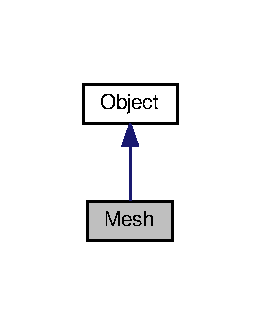
\includegraphics[width=125pt]{classMesh__inherit__graph}
\end{center}
\end{figure}


Collaboration diagram for Mesh\+:
\nopagebreak
\begin{figure}[H]
\begin{center}
\leavevmode
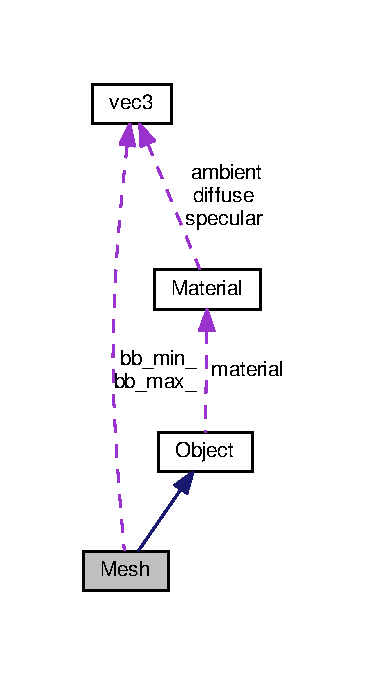
\includegraphics[width=177pt]{classMesh__coll__graph}
\end{center}
\end{figure}
\subsection*{Classes}
\begin{DoxyCompactItemize}
\item 
struct \hyperlink{structMesh_1_1Triangle}{Triangle}
\begin{DoxyCompactList}\small\item\em a triangle is specified by three indices and a normal \end{DoxyCompactList}\item 
struct \hyperlink{structMesh_1_1Vertex}{Vertex}
\begin{DoxyCompactList}\small\item\em a vertex consists of a position and a normal \end{DoxyCompactList}\end{DoxyCompactItemize}
\subsection*{Public Types}
\begin{DoxyCompactItemize}
\item 
enum \hyperlink{classMesh_aa4144c3cad2e62df26ad90131e59aa6a}{Draw\+\_\+mode} \{ \hyperlink{classMesh_aa4144c3cad2e62df26ad90131e59aa6aae58e62c20878ec327ed6409c7852b871}{F\+L\+AT}, 
\hyperlink{classMesh_aa4144c3cad2e62df26ad90131e59aa6aafc0cc7ddf5257c8d2a52d84573da372a}{P\+H\+O\+NG}
 \}\begin{DoxyCompactList}\small\item\em This type is used to choose between flat shading and Phong shading. \end{DoxyCompactList}
\end{DoxyCompactItemize}
\subsection*{Public Member Functions}
\begin{DoxyCompactItemize}
\item 
\hyperlink{classMesh_a58ef6d7fa08a5b8eef0c9b97d6c55e0d}{Mesh} (std\+::istream \&is, const std\+::string \&scene\+Path)
\item 
virtual bool \hyperlink{classMesh_a3d982c37d43eb5d3929b2de2b263d662}{intersect} (const \hyperlink{classRay}{Ray} \&\+\_\+ray, \hyperlink{classvec3}{vec3} \&\+\_\+intersection\+\_\+point, \hyperlink{classvec3}{vec3} \&\+\_\+intersection\+\_\+normal, double \&\+\_\+intersection\+\_\+t) const override
\item 
bool \hyperlink{classMesh_a77532d1e9aee1671d4ea38be1ed0d464}{read} (const std\+::string \&\+\_\+filename)
\begin{DoxyCompactList}\small\item\em Read mesh from an O\+FF file. \end{DoxyCompactList}\item 
void \hyperlink{classMesh_a4e9bedfc415b7135c9587f63535fcb6d}{compute\+\_\+normals} ()
\begin{DoxyCompactList}\small\item\em Compute normal vectors for triangles and vertices. \end{DoxyCompactList}\item 
void \hyperlink{classMesh_a303c102fd254ea32b366591aa00f6e8e}{compute\+\_\+bounding\+\_\+box} ()
\begin{DoxyCompactList}\small\item\em Compute the axis-\/aligned bounding box, store minimum and maximum point in bb\+\_\+min\+\_\+ and bb\+\_\+max\+\_\+. \end{DoxyCompactList}\item 
bool \hyperlink{classMesh_a5839749bb09a6bf09c56056016cc11b2}{intersect\+\_\+bounding\+\_\+box} (const \hyperlink{classRay}{Ray} \&\+\_\+ray) const 
\begin{DoxyCompactList}\small\item\em Does {\ttfamily \+\_\+ray} intersect the bounding box of the mesh? \end{DoxyCompactList}\item 
bool \hyperlink{classMesh_a9be7264791ff3de7dbf99f8548fb7725}{intersect\+\_\+triangle} (const \hyperlink{structMesh_1_1Triangle}{Triangle} \&\+\_\+triangle, const \hyperlink{classRay}{Ray} \&\+\_\+ray, \hyperlink{classvec3}{vec3} \&\+\_\+intersection\+\_\+point, \hyperlink{classvec3}{vec3} \&\+\_\+intersection\+\_\+normal, double \&\+\_\+intersection\+\_\+t) const 
\end{DoxyCompactItemize}
\subsection*{Private Attributes}
\begin{DoxyCompactItemize}
\item 
\hyperlink{classMesh_aa4144c3cad2e62df26ad90131e59aa6a}{Draw\+\_\+mode} \hyperlink{classMesh_a00bc30acf9fbbf37a6626aefeeae40ab}{draw\+\_\+mode\+\_\+}
\begin{DoxyCompactList}\small\item\em Does this mesh use flat or Phong shading? \end{DoxyCompactList}\item 
std\+::vector$<$ \hyperlink{structMesh_1_1Vertex}{Vertex} $>$ \hyperlink{classMesh_a986edf1ab1d37e517ff8adc928519528}{vertices\+\_\+}
\begin{DoxyCompactList}\small\item\em Array of vertices. \end{DoxyCompactList}\item 
std\+::vector$<$ \hyperlink{structMesh_1_1Triangle}{Triangle} $>$ \hyperlink{classMesh_a13455b3ace274f1d3d36ee45c7a3988d}{triangles\+\_\+}
\begin{DoxyCompactList}\small\item\em Array of triangles. \end{DoxyCompactList}\item 
\hyperlink{classvec3}{vec3} \hyperlink{classMesh_a92a3f0d35d2508cae425862f4d302943}{bb\+\_\+min\+\_\+}
\begin{DoxyCompactList}\small\item\em Minimum point of the bounding box. \end{DoxyCompactList}\item 
\hyperlink{classvec3}{vec3} \hyperlink{classMesh_acb17b74d4630a25eb2586a5d2c89975d}{bb\+\_\+max\+\_\+}
\begin{DoxyCompactList}\small\item\em Maximum point of the bounding box. \end{DoxyCompactList}\end{DoxyCompactItemize}
\subsection*{Additional Inherited Members}


\subsection{Detailed Description}
This class represents a simple triangle mesh, stored as an indexed face set, i.\+e., as an array of vertices and an array of triangles. 

\subsection{Member Enumeration Documentation}
\index{Mesh@{Mesh}!Draw\+\_\+mode@{Draw\+\_\+mode}}
\index{Draw\+\_\+mode@{Draw\+\_\+mode}!Mesh@{Mesh}}
\subsubsection[{\texorpdfstring{Draw\+\_\+mode}{Draw_mode}}]{\setlength{\rightskip}{0pt plus 5cm}enum {\bf Mesh\+::\+Draw\+\_\+mode}}\hypertarget{classMesh_aa4144c3cad2e62df26ad90131e59aa6a}{}\label{classMesh_aa4144c3cad2e62df26ad90131e59aa6a}


This type is used to choose between flat shading and Phong shading. 

\begin{Desc}
\item[Enumerator]\par
\begin{description}
\index{F\+L\+AT@{F\+L\+AT}!Mesh@{Mesh}}\index{Mesh@{Mesh}!F\+L\+AT@{F\+L\+AT}}\item[{\em 
F\+L\+AT\hypertarget{classMesh_aa4144c3cad2e62df26ad90131e59aa6aae58e62c20878ec327ed6409c7852b871}{}\label{classMesh_aa4144c3cad2e62df26ad90131e59aa6aae58e62c20878ec327ed6409c7852b871}
}]\index{P\+H\+O\+NG@{P\+H\+O\+NG}!Mesh@{Mesh}}\index{Mesh@{Mesh}!P\+H\+O\+NG@{P\+H\+O\+NG}}\item[{\em 
P\+H\+O\+NG\hypertarget{classMesh_aa4144c3cad2e62df26ad90131e59aa6aafc0cc7ddf5257c8d2a52d84573da372a}{}\label{classMesh_aa4144c3cad2e62df26ad90131e59aa6aafc0cc7ddf5257c8d2a52d84573da372a}
}]\end{description}
\end{Desc}


\subsection{Constructor \& Destructor Documentation}
\index{Mesh@{Mesh}!Mesh@{Mesh}}
\index{Mesh@{Mesh}!Mesh@{Mesh}}
\subsubsection[{\texorpdfstring{Mesh(std\+::istream \&is, const std\+::string \&scene\+Path)}{Mesh(std::istream &is, const std::string &scenePath)}}]{\setlength{\rightskip}{0pt plus 5cm}Mesh\+::\+Mesh (
\begin{DoxyParamCaption}
\item[{std\+::istream \&}]{is, }
\item[{const std\+::string \&}]{scene\+Path}
\end{DoxyParamCaption}
)}\hypertarget{classMesh_a58ef6d7fa08a5b8eef0c9b97d6c55e0d}{}\label{classMesh_a58ef6d7fa08a5b8eef0c9b97d6c55e0d}
Construct a mesh by parsing its path and properties from an input stream. The mesh path read from the file is relative to the scene file\textquotesingle{}s path \char`\"{}scene\+Path\char`\"{}. 

\subsection{Member Function Documentation}
\index{Mesh@{Mesh}!compute\+\_\+bounding\+\_\+box@{compute\+\_\+bounding\+\_\+box}}
\index{compute\+\_\+bounding\+\_\+box@{compute\+\_\+bounding\+\_\+box}!Mesh@{Mesh}}
\subsubsection[{\texorpdfstring{compute\+\_\+bounding\+\_\+box()}{compute_bounding_box()}}]{\setlength{\rightskip}{0pt plus 5cm}void Mesh\+::compute\+\_\+bounding\+\_\+box (
\begin{DoxyParamCaption}
{}
\end{DoxyParamCaption}
)}\hypertarget{classMesh_a303c102fd254ea32b366591aa00f6e8e}{}\label{classMesh_a303c102fd254ea32b366591aa00f6e8e}


Compute the axis-\/aligned bounding box, store minimum and maximum point in bb\+\_\+min\+\_\+ and bb\+\_\+max\+\_\+. 

\index{Mesh@{Mesh}!compute\+\_\+normals@{compute\+\_\+normals}}
\index{compute\+\_\+normals@{compute\+\_\+normals}!Mesh@{Mesh}}
\subsubsection[{\texorpdfstring{compute\+\_\+normals()}{compute_normals()}}]{\setlength{\rightskip}{0pt plus 5cm}void Mesh\+::compute\+\_\+normals (
\begin{DoxyParamCaption}
{}
\end{DoxyParamCaption}
)}\hypertarget{classMesh_a4e9bedfc415b7135c9587f63535fcb6d}{}\label{classMesh_a4e9bedfc415b7135c9587f63535fcb6d}


Compute normal vectors for triangles and vertices. 

\index{Mesh@{Mesh}!intersect@{intersect}}
\index{intersect@{intersect}!Mesh@{Mesh}}
\subsubsection[{\texorpdfstring{intersect(const Ray \&\+\_\+ray, vec3 \&\+\_\+intersection\+\_\+point, vec3 \&\+\_\+intersection\+\_\+normal, double \&\+\_\+intersection\+\_\+t) const override}{intersect(const Ray &_ray, vec3 &_intersection_point, vec3 &_intersection_normal, double &_intersection_t) const override}}]{\setlength{\rightskip}{0pt plus 5cm}bool Mesh\+::intersect (
\begin{DoxyParamCaption}
\item[{const {\bf Ray} \&}]{\+\_\+ray, }
\item[{{\bf vec3} \&}]{\+\_\+intersection\+\_\+point, }
\item[{{\bf vec3} \&}]{\+\_\+intersection\+\_\+normal, }
\item[{double \&}]{\+\_\+intersection\+\_\+t}
\end{DoxyParamCaption}
) const\hspace{0.3cm}{\ttfamily [override]}, {\ttfamily [virtual]}}\hypertarget{classMesh_a3d982c37d43eb5d3929b2de2b263d662}{}\label{classMesh_a3d982c37d43eb5d3929b2de2b263d662}
Intersect mesh with ray (calls ray-\/triangle intersection) If {\ttfamily \+\_\+ray} intersects a face of the mesh, it provides the following results\+: 
\begin{DoxyParams}[1]{Parameters}
\mbox{\tt in}  & {\em \+\_\+ray} & the ray to intersect the mesh with \\
\hline
\mbox{\tt out}  & {\em \+\_\+intersection\+\_\+point} & the point of intersection \\
\hline
\mbox{\tt out}  & {\em \+\_\+intersection\+\_\+normal} & the surface normal at intersection point \\
\hline
\mbox{\tt out}  & {\em \+\_\+intersection\+\_\+t} & ray parameter at the intersection point \\
\hline
\end{DoxyParams}


Implements \hyperlink{structObject_ac6549d30793a9b3da070234bf10c7e91}{Object}.

\index{Mesh@{Mesh}!intersect\+\_\+bounding\+\_\+box@{intersect\+\_\+bounding\+\_\+box}}
\index{intersect\+\_\+bounding\+\_\+box@{intersect\+\_\+bounding\+\_\+box}!Mesh@{Mesh}}
\subsubsection[{\texorpdfstring{intersect\+\_\+bounding\+\_\+box(const Ray \&\+\_\+ray) const }{intersect_bounding_box(const Ray &_ray) const }}]{\setlength{\rightskip}{0pt plus 5cm}bool Mesh\+::intersect\+\_\+bounding\+\_\+box (
\begin{DoxyParamCaption}
\item[{const {\bf Ray} \&}]{\+\_\+ray}
\end{DoxyParamCaption}
) const}\hypertarget{classMesh_a5839749bb09a6bf09c56056016cc11b2}{}\label{classMesh_a5839749bb09a6bf09c56056016cc11b2}


Does {\ttfamily \+\_\+ray} intersect the bounding box of the mesh? 

\index{Mesh@{Mesh}!intersect\+\_\+triangle@{intersect\+\_\+triangle}}
\index{intersect\+\_\+triangle@{intersect\+\_\+triangle}!Mesh@{Mesh}}
\subsubsection[{\texorpdfstring{intersect\+\_\+triangle(const Triangle \&\+\_\+triangle, const Ray \&\+\_\+ray, vec3 \&\+\_\+intersection\+\_\+point, vec3 \&\+\_\+intersection\+\_\+normal, double \&\+\_\+intersection\+\_\+t) const }{intersect_triangle(const Triangle &_triangle, const Ray &_ray, vec3 &_intersection_point, vec3 &_intersection_normal, double &_intersection_t) const }}]{\setlength{\rightskip}{0pt plus 5cm}bool Mesh\+::intersect\+\_\+triangle (
\begin{DoxyParamCaption}
\item[{const {\bf Triangle} \&}]{\+\_\+triangle, }
\item[{const {\bf Ray} \&}]{\+\_\+ray, }
\item[{{\bf vec3} \&}]{\+\_\+intersection\+\_\+point, }
\item[{{\bf vec3} \&}]{\+\_\+intersection\+\_\+normal, }
\item[{double \&}]{\+\_\+intersection\+\_\+t}
\end{DoxyParamCaption}
) const}\hypertarget{classMesh_a9be7264791ff3de7dbf99f8548fb7725}{}\label{classMesh_a9be7264791ff3de7dbf99f8548fb7725}
Intersect a triangle with a ray. Return whether there is an intersection. If there is an intersection, store intersection data. This function overrides \hyperlink{structObject_ac6549d30793a9b3da070234bf10c7e91}{Object\+::intersect()}. 
\begin{DoxyParams}[1]{Parameters}
\mbox{\tt in}  & {\em \+\_\+triangle} & the triangle to be intersected \\
\hline
\mbox{\tt in}  & {\em \+\_\+ray} & the ray to intersect the triangle with \\
\hline
\mbox{\tt out}  & {\em \+\_\+intersection\+\_\+point} & the point of intersection \\
\hline
\mbox{\tt out}  & {\em \+\_\+intersection\+\_\+normal} & the surface normal at intersection point \\
\hline
\mbox{\tt out}  & {\em \+\_\+intersection\+\_\+t} & ray parameter at the intersection point \\
\hline
\end{DoxyParams}
\index{Mesh@{Mesh}!read@{read}}
\index{read@{read}!Mesh@{Mesh}}
\subsubsection[{\texorpdfstring{read(const std\+::string \&\+\_\+filename)}{read(const std::string &_filename)}}]{\setlength{\rightskip}{0pt plus 5cm}bool Mesh\+::read (
\begin{DoxyParamCaption}
\item[{const std\+::string \&}]{\+\_\+filename}
\end{DoxyParamCaption}
)}\hypertarget{classMesh_a77532d1e9aee1671d4ea38be1ed0d464}{}\label{classMesh_a77532d1e9aee1671d4ea38be1ed0d464}


Read mesh from an O\+FF file. 



\subsection{Member Data Documentation}
\index{Mesh@{Mesh}!bb\+\_\+max\+\_\+@{bb\+\_\+max\+\_\+}}
\index{bb\+\_\+max\+\_\+@{bb\+\_\+max\+\_\+}!Mesh@{Mesh}}
\subsubsection[{\texorpdfstring{bb\+\_\+max\+\_\+}{bb_max_}}]{\setlength{\rightskip}{0pt plus 5cm}{\bf vec3} Mesh\+::bb\+\_\+max\+\_\+\hspace{0.3cm}{\ttfamily [private]}}\hypertarget{classMesh_acb17b74d4630a25eb2586a5d2c89975d}{}\label{classMesh_acb17b74d4630a25eb2586a5d2c89975d}


Maximum point of the bounding box. 

\index{Mesh@{Mesh}!bb\+\_\+min\+\_\+@{bb\+\_\+min\+\_\+}}
\index{bb\+\_\+min\+\_\+@{bb\+\_\+min\+\_\+}!Mesh@{Mesh}}
\subsubsection[{\texorpdfstring{bb\+\_\+min\+\_\+}{bb_min_}}]{\setlength{\rightskip}{0pt plus 5cm}{\bf vec3} Mesh\+::bb\+\_\+min\+\_\+\hspace{0.3cm}{\ttfamily [private]}}\hypertarget{classMesh_a92a3f0d35d2508cae425862f4d302943}{}\label{classMesh_a92a3f0d35d2508cae425862f4d302943}


Minimum point of the bounding box. 

\index{Mesh@{Mesh}!draw\+\_\+mode\+\_\+@{draw\+\_\+mode\+\_\+}}
\index{draw\+\_\+mode\+\_\+@{draw\+\_\+mode\+\_\+}!Mesh@{Mesh}}
\subsubsection[{\texorpdfstring{draw\+\_\+mode\+\_\+}{draw_mode_}}]{\setlength{\rightskip}{0pt plus 5cm}{\bf Draw\+\_\+mode} Mesh\+::draw\+\_\+mode\+\_\+\hspace{0.3cm}{\ttfamily [private]}}\hypertarget{classMesh_a00bc30acf9fbbf37a6626aefeeae40ab}{}\label{classMesh_a00bc30acf9fbbf37a6626aefeeae40ab}


Does this mesh use flat or Phong shading? 

\index{Mesh@{Mesh}!triangles\+\_\+@{triangles\+\_\+}}
\index{triangles\+\_\+@{triangles\+\_\+}!Mesh@{Mesh}}
\subsubsection[{\texorpdfstring{triangles\+\_\+}{triangles_}}]{\setlength{\rightskip}{0pt plus 5cm}std\+::vector$<${\bf Triangle}$>$ Mesh\+::triangles\+\_\+\hspace{0.3cm}{\ttfamily [private]}}\hypertarget{classMesh_a13455b3ace274f1d3d36ee45c7a3988d}{}\label{classMesh_a13455b3ace274f1d3d36ee45c7a3988d}


Array of triangles. 

\index{Mesh@{Mesh}!vertices\+\_\+@{vertices\+\_\+}}
\index{vertices\+\_\+@{vertices\+\_\+}!Mesh@{Mesh}}
\subsubsection[{\texorpdfstring{vertices\+\_\+}{vertices_}}]{\setlength{\rightskip}{0pt plus 5cm}std\+::vector$<${\bf Vertex}$>$ Mesh\+::vertices\+\_\+\hspace{0.3cm}{\ttfamily [private]}}\hypertarget{classMesh_a986edf1ab1d37e517ff8adc928519528}{}\label{classMesh_a986edf1ab1d37e517ff8adc928519528}


Array of vertices. 



The documentation for this class was generated from the following files\+:\begin{DoxyCompactItemize}
\item 
/home/eason/\+Desktop/assignment\+\_\+0/src/\hyperlink{Mesh_8h}{Mesh.\+h}\item 
/home/eason/\+Desktop/assignment\+\_\+0/src/\hyperlink{Mesh_8cpp}{Mesh.\+cpp}\end{DoxyCompactItemize}

\hypertarget{structObject}{}\section{Object Class Reference}
\label{structObject}\index{Object@{Object}}


{\ttfamily \#include $<$Object.\+h$>$}



Inheritance diagram for Object\+:
% FIG 0


Collaboration diagram for Object\+:
% FIG 1
\subsection*{Public Member Functions}
\begin{DoxyCompactItemize}
\item 
\hyperlink{structObject_a40860402e64d8008fb42329df7097cdb}{Object} ()
\begin{DoxyCompactList}\small\item\em Default (empty) constructor. \end{DoxyCompactList}\item 
virtual \hyperlink{structObject_aa3e791419d84c4c346ef9499513b8e00}{$\sim$\+Object} ()
\item 
virtual bool \hyperlink{structObject_ac6549d30793a9b3da070234bf10c7e91}{intersect} (const \hyperlink{classRay}{Ray} \&\+\_\+ray, \hyperlink{classvec3}{vec3} \&\+\_\+intersection\+\_\+point, \hyperlink{classvec3}{vec3} \&\+\_\+intersection\+\_\+normal, double \&\+\_\+intersection\+\_\+t) const =0
\item 
virtual void \hyperlink{structObject_ae7828b080c96e2226f3dc19823161d41}{parse} (std\+::istream \&is)
\begin{DoxyCompactList}\small\item\em parse object properties from an input stream \end{DoxyCompactList}\end{DoxyCompactItemize}
\subsection*{Public Attributes}
\begin{DoxyCompactItemize}
\item 
\hyperlink{structMaterial}{Material} \hyperlink{structObject_a2f63d05a9a9264e1b6c388fa4bba4e91}{material}
\begin{DoxyCompactList}\small\item\em The material of this object. \end{DoxyCompactList}\end{DoxyCompactItemize}
\subsection*{Static Public Attributes}
\begin{DoxyCompactItemize}
\item 
static constexpr double \hyperlink{structObject_a68971b3c931312e76077de7f8597a6d4}{N\+O\+\_\+\+I\+N\+T\+E\+R\+S\+E\+C\+T\+I\+ON} = std\+::numeric\+\_\+limits$<$double$>$\+::\hyperlink{vec3_8h_a88bf317d8d46ef981cc71e72eb77b184}{max}()
\end{DoxyCompactItemize}


\subsection{Detailed Description}
This class implements an abstract class for an object. Every derived object type will inherit the material property, and it will have to override the virtual function \hyperlink{structObject_ac6549d30793a9b3da070234bf10c7e91}{Object\+::intersect()}. 

\subsection{Constructor \& Destructor Documentation}
\index{Object@{Object}!Object@{Object}}
\index{Object@{Object}!Object@{Object}}
\subsubsection[{\texorpdfstring{Object()}{Object()}}]{\setlength{\rightskip}{0pt plus 5cm}Object\+::\+Object (
\begin{DoxyParamCaption}
{}
\end{DoxyParamCaption}
)\hspace{0.3cm}{\ttfamily [inline]}}\hypertarget{structObject_a40860402e64d8008fb42329df7097cdb}{}\label{structObject_a40860402e64d8008fb42329df7097cdb}


Default (empty) constructor. 

\index{Object@{Object}!````~Object@{$\sim$\+Object}}
\index{````~Object@{$\sim$\+Object}!Object@{Object}}
\subsubsection[{\texorpdfstring{$\sim$\+Object()}{~Object()}}]{\setlength{\rightskip}{0pt plus 5cm}virtual Object\+::$\sim$\+Object (
\begin{DoxyParamCaption}
{}
\end{DoxyParamCaption}
)\hspace{0.3cm}{\ttfamily [inline]}, {\ttfamily [virtual]}}\hypertarget{structObject_aa3e791419d84c4c346ef9499513b8e00}{}\label{structObject_aa3e791419d84c4c346ef9499513b8e00}
Destructor (if a class has virtual functions, then its destructor has to be virtual as well). 

\subsection{Member Function Documentation}
\index{Object@{Object}!intersect@{intersect}}
\index{intersect@{intersect}!Object@{Object}}
\subsubsection[{\texorpdfstring{intersect(const Ray \&\+\_\+ray, vec3 \&\+\_\+intersection\+\_\+point, vec3 \&\+\_\+intersection\+\_\+normal, double \&\+\_\+intersection\+\_\+t) const =0}{intersect(const Ray &_ray, vec3 &_intersection_point, vec3 &_intersection_normal, double &_intersection_t) const =0}}]{\setlength{\rightskip}{0pt plus 5cm}virtual bool Object\+::intersect (
\begin{DoxyParamCaption}
\item[{const {\bf Ray} \&}]{\+\_\+ray, }
\item[{{\bf vec3} \&}]{\+\_\+intersection\+\_\+point, }
\item[{{\bf vec3} \&}]{\+\_\+intersection\+\_\+normal, }
\item[{double \&}]{\+\_\+intersection\+\_\+t}
\end{DoxyParamCaption}
) const\hspace{0.3cm}{\ttfamily [pure virtual]}}\hypertarget{structObject_ac6549d30793a9b3da070234bf10c7e91}{}\label{structObject_ac6549d30793a9b3da070234bf10c7e91}
Intersect the object with {\ttfamily \+\_\+ray}, return whether there is an intersection. If {\ttfamily \+\_\+ray} intersects the object, provide the following results\+: 
\begin{DoxyParams}[1]{Parameters}
\mbox{\tt in}  & {\em \+\_\+ray} & the ray to intersect the object with \\
\hline
\mbox{\tt out}  & {\em \+\_\+intersection\+\_\+point} & the point of intersection \\
\hline
\mbox{\tt out}  & {\em \+\_\+intersection\+\_\+normal} & the surface normal at intersection point \\
\hline
\mbox{\tt out}  & {\em \+\_\+intersection\+\_\+t} & ray parameter at intersection point \\
\hline
\end{DoxyParams}


Implemented in \hyperlink{classCylinder_a0ae732b1b669bbeb9eb83ee7395a5add}{Cylinder}, \hyperlink{classMesh_a3d982c37d43eb5d3929b2de2b263d662}{Mesh}, \hyperlink{classPlane_ab146bb10ad52e8535dad25d531c43b86}{Plane}, and \hyperlink{classSphere_a6650f14281c43b799d9ae0c0b690b1bd}{Sphere}.

\index{Object@{Object}!parse@{parse}}
\index{parse@{parse}!Object@{Object}}
\subsubsection[{\texorpdfstring{parse(std\+::istream \&is)}{parse(std::istream &is)}}]{\setlength{\rightskip}{0pt plus 5cm}virtual void Object\+::parse (
\begin{DoxyParamCaption}
\item[{std\+::istream \&}]{is}
\end{DoxyParamCaption}
)\hspace{0.3cm}{\ttfamily [inline]}, {\ttfamily [virtual]}}\hypertarget{structObject_ae7828b080c96e2226f3dc19823161d41}{}\label{structObject_ae7828b080c96e2226f3dc19823161d41}


parse object properties from an input stream 



Reimplemented in \hyperlink{classCylinder_a15050a6257a624cae1566a949b03b7da}{Cylinder}, \hyperlink{classPlane_af5361222d1aa404fc720d7b4b68a634c}{Plane}, and \hyperlink{classSphere_aa55e3407f148feb451866bc39907f6fb}{Sphere}.



\subsection{Member Data Documentation}
\index{Object@{Object}!material@{material}}
\index{material@{material}!Object@{Object}}
\subsubsection[{\texorpdfstring{material}{material}}]{\setlength{\rightskip}{0pt plus 5cm}{\bf Material} Object\+::material}\hypertarget{structObject_a2f63d05a9a9264e1b6c388fa4bba4e91}{}\label{structObject_a2f63d05a9a9264e1b6c388fa4bba4e91}


The material of this object. 

\index{Object@{Object}!N\+O\+\_\+\+I\+N\+T\+E\+R\+S\+E\+C\+T\+I\+ON@{N\+O\+\_\+\+I\+N\+T\+E\+R\+S\+E\+C\+T\+I\+ON}}
\index{N\+O\+\_\+\+I\+N\+T\+E\+R\+S\+E\+C\+T\+I\+ON@{N\+O\+\_\+\+I\+N\+T\+E\+R\+S\+E\+C\+T\+I\+ON}!Object@{Object}}
\subsubsection[{\texorpdfstring{N\+O\+\_\+\+I\+N\+T\+E\+R\+S\+E\+C\+T\+I\+ON}{NO_INTERSECTION}}]{\setlength{\rightskip}{0pt plus 5cm}constexpr double Object\+::\+N\+O\+\_\+\+I\+N\+T\+E\+R\+S\+E\+C\+T\+I\+ON = std\+::numeric\+\_\+limits$<$double$>$\+::{\bf max}()\hspace{0.3cm}{\ttfamily [static]}}\hypertarget{structObject_a68971b3c931312e76077de7f8597a6d4}{}\label{structObject_a68971b3c931312e76077de7f8597a6d4}


The documentation for this class was generated from the following file\+:\begin{DoxyCompactItemize}
\item 
/home/eason/\+Desktop/\+E\+P\+F\+L\+\_\+\+C\+G/assignment\+\_\+2/src/\hyperlink{Object_8h}{Object.\+h}\end{DoxyCompactItemize}

\hypertarget{classPlane}{}\section{Plane Class Reference}
\label{classPlane}\index{Plane@{Plane}}


{\ttfamily \#include $<$Plane.\+h$>$}



Inheritance diagram for Plane\+:
% FIG 0


Collaboration diagram for Plane\+:
% FIG 1
\subsection*{Public Member Functions}
\begin{DoxyCompactItemize}
\item 
\hyperlink{classPlane_a6ce42dd3bf06b497256454534f582a80}{Plane} (const \hyperlink{classvec3}{vec3} \&\+\_\+center=\hyperlink{classvec3}{vec3}(0, 0, 0), const \hyperlink{classvec3}{vec3} \&\+\_\+normal=\hyperlink{classvec3}{vec3}(0, 1, 0))
\begin{DoxyCompactList}\small\item\em constructor \end{DoxyCompactList}\item 
\hyperlink{classPlane_a5236597c4a6324126e8746ecb4af1535}{Plane} (std\+::istream \&is)
\begin{DoxyCompactList}\small\item\em Construct a plane with parameters parsed from an input stream. \end{DoxyCompactList}\item 
virtual bool \hyperlink{classPlane_ab146bb10ad52e8535dad25d531c43b86}{intersect} (const \hyperlink{classRay}{Ray} \&\+\_\+ray, \hyperlink{classvec3}{vec3} \&\+\_\+intersection\+\_\+point, \hyperlink{classvec3}{vec3} \&\+\_\+intersection\+\_\+normal, double \&\+\_\+intersection\+\_\+t) const override
\item 
virtual void \hyperlink{classPlane_af5361222d1aa404fc720d7b4b68a634c}{parse} (std\+::istream \&is) override
\begin{DoxyCompactList}\small\item\em parse plane from an input stream \end{DoxyCompactList}\end{DoxyCompactItemize}
\subsection*{Private Attributes}
\begin{DoxyCompactItemize}
\item 
\hyperlink{classvec3}{vec3} \hyperlink{classPlane_a366eef1f4daccfc48ccd824cca63a026}{center}
\begin{DoxyCompactList}\small\item\em one (arbitrary) point on the plane \end{DoxyCompactList}\item 
\hyperlink{classvec3}{vec3} \hyperlink{classPlane_ac3a6d80b28df1dd0ef7867663227c937}{normal}
\begin{DoxyCompactList}\small\item\em normal vector of the plane \end{DoxyCompactList}\end{DoxyCompactItemize}
\subsection*{Additional Inherited Members}


\subsection{Detailed Description}
This class implements a simple plane object. A plane is specified by a center point and a normal vector. This class overrides the intersection method \hyperlink{structObject_ac6549d30793a9b3da070234bf10c7e91}{Object\+::intersect()}. 

\subsection{Constructor \& Destructor Documentation}
\index{Plane@{Plane}!Plane@{Plane}}
\index{Plane@{Plane}!Plane@{Plane}}
\subsubsection[{\texorpdfstring{Plane(const vec3 \&\+\_\+center=vec3(0, 0, 0), const vec3 \&\+\_\+normal=vec3(0, 1, 0))}{Plane(const vec3 &_center=vec3(0, 0, 0), const vec3 &_normal=vec3(0, 1, 0))}}]{\setlength{\rightskip}{0pt plus 5cm}Plane\+::\+Plane (
\begin{DoxyParamCaption}
\item[{const {\bf vec3} \&}]{\+\_\+center = {\ttfamily {\bf vec3}(0,0,0)}, }
\item[{const {\bf vec3} \&}]{\+\_\+normal = {\ttfamily {\bf vec3}(0,1,0)}}
\end{DoxyParamCaption}
)}\hypertarget{classPlane_a6ce42dd3bf06b497256454534f582a80}{}\label{classPlane_a6ce42dd3bf06b497256454534f582a80}


constructor 

\index{Plane@{Plane}!Plane@{Plane}}
\index{Plane@{Plane}!Plane@{Plane}}
\subsubsection[{\texorpdfstring{Plane(std\+::istream \&is)}{Plane(std::istream &is)}}]{\setlength{\rightskip}{0pt plus 5cm}Plane\+::\+Plane (
\begin{DoxyParamCaption}
\item[{std\+::istream \&}]{is}
\end{DoxyParamCaption}
)\hspace{0.3cm}{\ttfamily [inline]}}\hypertarget{classPlane_a5236597c4a6324126e8746ecb4af1535}{}\label{classPlane_a5236597c4a6324126e8746ecb4af1535}


Construct a plane with parameters parsed from an input stream. 



\subsection{Member Function Documentation}
\index{Plane@{Plane}!intersect@{intersect}}
\index{intersect@{intersect}!Plane@{Plane}}
\subsubsection[{\texorpdfstring{intersect(const Ray \&\+\_\+ray, vec3 \&\+\_\+intersection\+\_\+point, vec3 \&\+\_\+intersection\+\_\+normal, double \&\+\_\+intersection\+\_\+t) const override}{intersect(const Ray &_ray, vec3 &_intersection_point, vec3 &_intersection_normal, double &_intersection_t) const override}}]{\setlength{\rightskip}{0pt plus 5cm}bool Plane\+::intersect (
\begin{DoxyParamCaption}
\item[{const {\bf Ray} \&}]{\+\_\+ray, }
\item[{{\bf vec3} \&}]{\+\_\+intersection\+\_\+point, }
\item[{{\bf vec3} \&}]{\+\_\+intersection\+\_\+normal, }
\item[{double \&}]{\+\_\+intersection\+\_\+t}
\end{DoxyParamCaption}
) const\hspace{0.3cm}{\ttfamily [override]}, {\ttfamily [virtual]}}\hypertarget{classPlane_ab146bb10ad52e8535dad25d531c43b86}{}\label{classPlane_ab146bb10ad52e8535dad25d531c43b86}
Compute the intersection of the plane with {\ttfamily \+\_\+ray}. Return whether there is an intersection. If there is one, return the intersection data. This function overrides \hyperlink{structObject_ac6549d30793a9b3da070234bf10c7e91}{Object\+::intersect()}. 
\begin{DoxyParams}[1]{Parameters}
\mbox{\tt in}  & {\em \+\_\+ray} & the ray to intersect the plane with \\
\hline
\mbox{\tt out}  & {\em \+\_\+intersection\+\_\+point} & position of the intersection \\
\hline
\mbox{\tt out}  & {\em \+\_\+intersection\+\_\+normal} & normal vector at the intersection point \\
\hline
\mbox{\tt out}  & {\em \+\_\+intersection\+\_\+t} & ray parameter at the intesection point \\
\hline
\end{DoxyParams}


Implements \hyperlink{structObject_ac6549d30793a9b3da070234bf10c7e91}{Object}.

\index{Plane@{Plane}!parse@{parse}}
\index{parse@{parse}!Plane@{Plane}}
\subsubsection[{\texorpdfstring{parse(std\+::istream \&is) override}{parse(std::istream &is) override}}]{\setlength{\rightskip}{0pt plus 5cm}virtual void Plane\+::parse (
\begin{DoxyParamCaption}
\item[{std\+::istream \&}]{is}
\end{DoxyParamCaption}
)\hspace{0.3cm}{\ttfamily [inline]}, {\ttfamily [override]}, {\ttfamily [virtual]}}\hypertarget{classPlane_af5361222d1aa404fc720d7b4b68a634c}{}\label{classPlane_af5361222d1aa404fc720d7b4b68a634c}


parse plane from an input stream 



Reimplemented from \hyperlink{structObject_ae7828b080c96e2226f3dc19823161d41}{Object}.



\subsection{Member Data Documentation}
\index{Plane@{Plane}!center@{center}}
\index{center@{center}!Plane@{Plane}}
\subsubsection[{\texorpdfstring{center}{center}}]{\setlength{\rightskip}{0pt plus 5cm}{\bf vec3} Plane\+::center\hspace{0.3cm}{\ttfamily [private]}}\hypertarget{classPlane_a366eef1f4daccfc48ccd824cca63a026}{}\label{classPlane_a366eef1f4daccfc48ccd824cca63a026}


one (arbitrary) point on the plane 

\index{Plane@{Plane}!normal@{normal}}
\index{normal@{normal}!Plane@{Plane}}
\subsubsection[{\texorpdfstring{normal}{normal}}]{\setlength{\rightskip}{0pt plus 5cm}{\bf vec3} Plane\+::normal\hspace{0.3cm}{\ttfamily [private]}}\hypertarget{classPlane_ac3a6d80b28df1dd0ef7867663227c937}{}\label{classPlane_ac3a6d80b28df1dd0ef7867663227c937}


normal vector of the plane 



The documentation for this class was generated from the following files\+:\begin{DoxyCompactItemize}
\item 
/home/eason/\+Desktop/\+E\+P\+F\+L\+\_\+\+C\+G/assignment\+\_\+0/src/\hyperlink{Plane_8h}{Plane.\+h}\item 
/home/eason/\+Desktop/\+E\+P\+F\+L\+\_\+\+C\+G/assignment\+\_\+0/src/\hyperlink{Plane_8cpp}{Plane.\+cpp}\end{DoxyCompactItemize}

\hypertarget{classRay}{}\section{Ray Class Reference}
\label{classRay}\index{Ray@{Ray}}


{\ttfamily \#include $<$Ray.\+h$>$}



Collaboration diagram for Ray\+:
\nopagebreak
\begin{figure}[H]
\begin{center}
\leavevmode
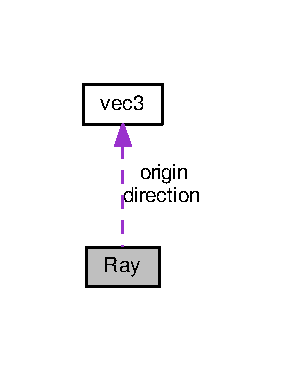
\includegraphics[width=136pt]{classRay__coll__graph}
\end{center}
\end{figure}
\subsection*{Public Member Functions}
\begin{DoxyCompactItemize}
\item 
\hyperlink{classRay_a773588948dfa8469c81f43907f6a7c63}{Ray} (const \hyperlink{classvec3}{vec3} \&\+\_\+origin=\hyperlink{classvec3}{vec3}(0, 0, 0), const \hyperlink{classvec3}{vec3} \&\+\_\+direction=\hyperlink{classvec3}{vec3}(0, 0, 1))
\begin{DoxyCompactList}\small\item\em Constructor with origin and direction. Direction will be normalized. \end{DoxyCompactList}\item 
\hyperlink{classvec3}{vec3} \hyperlink{classRay_adcb42927ac5d583e1296d2ec4e5b8b1a}{operator()} (double \+\_\+t) const 
\end{DoxyCompactItemize}
\subsection*{Public Attributes}
\begin{DoxyCompactItemize}
\item 
\hyperlink{classvec3}{vec3} \hyperlink{classRay_a3677f264c55cbe2f2cf450f9e0efa241}{origin}
\begin{DoxyCompactList}\small\item\em origin of the ray \end{DoxyCompactList}\item 
\hyperlink{classvec3}{vec3} \hyperlink{classRay_a2b864cd91328207dc66e3ab4cd1e1e36}{direction}
\begin{DoxyCompactList}\small\item\em direction of the ray (should be normalized) \end{DoxyCompactList}\end{DoxyCompactItemize}


\subsection{Detailed Description}
This class implements a ray, specified by its origin and direction. It provides a convenient function to compute the point ray(t) at a specific ray paramter t. 

\subsection{Constructor \& Destructor Documentation}
\index{Ray@{Ray}!Ray@{Ray}}
\index{Ray@{Ray}!Ray@{Ray}}
\subsubsection[{\texorpdfstring{Ray(const vec3 \&\+\_\+origin=vec3(0, 0, 0), const vec3 \&\+\_\+direction=vec3(0, 0, 1))}{Ray(const vec3 &_origin=vec3(0, 0, 0), const vec3 &_direction=vec3(0, 0, 1))}}]{\setlength{\rightskip}{0pt plus 5cm}Ray\+::\+Ray (
\begin{DoxyParamCaption}
\item[{const {\bf vec3} \&}]{\+\_\+origin = {\ttfamily {\bf vec3}(0,0,0)}, }
\item[{const {\bf vec3} \&}]{\+\_\+direction = {\ttfamily {\bf vec3}(0,0,1)}}
\end{DoxyParamCaption}
)\hspace{0.3cm}{\ttfamily [inline]}}\hypertarget{classRay_a773588948dfa8469c81f43907f6a7c63}{}\label{classRay_a773588948dfa8469c81f43907f6a7c63}


Constructor with origin and direction. Direction will be normalized. 



\subsection{Member Function Documentation}
\index{Ray@{Ray}!operator()@{operator()}}
\index{operator()@{operator()}!Ray@{Ray}}
\subsubsection[{\texorpdfstring{operator()(double \+\_\+t) const }{operator()(double _t) const }}]{\setlength{\rightskip}{0pt plus 5cm}{\bf vec3} Ray\+::operator() (
\begin{DoxyParamCaption}
\item[{double}]{\+\_\+t}
\end{DoxyParamCaption}
) const\hspace{0.3cm}{\ttfamily [inline]}}\hypertarget{classRay_adcb42927ac5d583e1296d2ec4e5b8b1a}{}\label{classRay_adcb42927ac5d583e1296d2ec4e5b8b1a}
Compute the point on the ray at the parameter {\ttfamily \+\_\+t}, which is origin + \+\_\+t$\ast$direction. 

\subsection{Member Data Documentation}
\index{Ray@{Ray}!direction@{direction}}
\index{direction@{direction}!Ray@{Ray}}
\subsubsection[{\texorpdfstring{direction}{direction}}]{\setlength{\rightskip}{0pt plus 5cm}{\bf vec3} Ray\+::direction}\hypertarget{classRay_a2b864cd91328207dc66e3ab4cd1e1e36}{}\label{classRay_a2b864cd91328207dc66e3ab4cd1e1e36}


direction of the ray (should be normalized) 

\index{Ray@{Ray}!origin@{origin}}
\index{origin@{origin}!Ray@{Ray}}
\subsubsection[{\texorpdfstring{origin}{origin}}]{\setlength{\rightskip}{0pt plus 5cm}{\bf vec3} Ray\+::origin}\hypertarget{classRay_a3677f264c55cbe2f2cf450f9e0efa241}{}\label{classRay_a3677f264c55cbe2f2cf450f9e0efa241}


origin of the ray 



The documentation for this class was generated from the following file\+:\begin{DoxyCompactItemize}
\item 
/home/eason/\+Desktop/assignment\+\_\+0/src/\hyperlink{Ray_8h}{Ray.\+h}\end{DoxyCompactItemize}

\hypertarget{classScene}{}\section{Scene Class Reference}
\label{classScene}\index{Scene@{Scene}}


{\ttfamily \#include $<$Scene.\+h$>$}



Collaboration diagram for Scene\+:
% FIG 0
\subsection*{Public Member Functions}
\begin{DoxyCompactItemize}
\item 
\hyperlink{classScene_a53cd40de123db36ab62763523ec0fc41}{Scene} (const std\+::string \&path)
\begin{DoxyCompactList}\small\item\em Constructor loads scene from file. \end{DoxyCompactList}\item 
\hyperlink{classImage}{Image} \hyperlink{classScene_aeaecd6069dfc02986fd04c9a8f905e89}{render} ()
\begin{DoxyCompactList}\small\item\em Allocate image and raytrace the scene. \end{DoxyCompactList}\item 
\hyperlink{classvec3}{vec3} \hyperlink{classScene_aee2e562b23da56880ea30e33f9e76e1b}{trace} (const \hyperlink{classRay}{Ray} \&\+\_\+ray, int \+\_\+depth)
\begin{DoxyCompactList}\small\item\em Determine the color seen by a viewing ray. \end{DoxyCompactList}\item 
bool \hyperlink{classScene_addfa0f2a14f2593e7f91dab0d5627990}{intersect} (const \hyperlink{classRay}{Ray} \&\+\_\+ray, \hyperlink{Object_8h_ad537f5b7b240eca7da458a29bbb47b9e}{Object\+\_\+ptr} \&, \hyperlink{classvec3}{vec3} \&\+\_\+point, \hyperlink{classvec3}{vec3} \&\+\_\+normal, double \&\+\_\+t)
\begin{DoxyCompactList}\small\item\em Computes the closest intersection point between a ray and all objects in the scene. \end{DoxyCompactList}\item 
\hyperlink{classvec3}{vec3} \hyperlink{classScene_a8c3c270f36a5e73805d925763450de7c}{lighting} (const \hyperlink{classvec3}{vec3} \&\+\_\+point, const \hyperlink{classvec3}{vec3} \&\+\_\+normal, const \hyperlink{classvec3}{vec3} \&\+\_\+view, const \hyperlink{structMaterial}{Material} \&\+\_\+material)
\begin{DoxyCompactList}\small\item\em Computes the phong lighting for a given object intersection. \end{DoxyCompactList}\item 
void \hyperlink{classScene_a15d828d5f43ff11466712b9203082316}{read} (const std\+::string \&filename)
\item 
size\+\_\+t \hyperlink{classScene_a27b9b9e915a87fd7736dd82d71da372a}{num\+Objects} () const 
\end{DoxyCompactItemize}
\subsection*{Private Attributes}
\begin{DoxyCompactItemize}
\item 
\hyperlink{classCamera}{Camera} \hyperlink{classScene_afed13ec4ba2d7ab75b273d507911b498}{camera}
\begin{DoxyCompactList}\small\item\em camera stores eye position, view direction, and can generate primary rays \end{DoxyCompactList}\item 
std\+::vector$<$ \hyperlink{structLight}{Light} $>$ \hyperlink{classScene_ab3625e4ac3c6e47156edd23e2421e828}{lights}
\begin{DoxyCompactList}\small\item\em array for all lights in the scene \end{DoxyCompactList}\item 
std\+::vector$<$ std\+::unique\+\_\+ptr$<$ \hyperlink{structObject}{Object} $>$ $>$ \hyperlink{classScene_abbd6f5b3a4639c3b089037519085bf86}{objects}
\begin{DoxyCompactList}\small\item\em array for all the objects in the scene \end{DoxyCompactList}\item 
int \hyperlink{classScene_a9150039f4d2c46a617b51c7920142d52}{max\+\_\+depth} = 0
\begin{DoxyCompactList}\small\item\em max recursion depth for mirroring \end{DoxyCompactList}\item 
\hyperlink{classvec3}{vec3} \hyperlink{classScene_ab2f20cf753edf2f92fec9b1ad7c9b93e}{background} = \hyperlink{classvec3}{vec3}(0, 0, 0)
\begin{DoxyCompactList}\small\item\em background color \end{DoxyCompactList}\item 
\hyperlink{classvec3}{vec3} \hyperlink{classScene_a8809b5fcac40d60ab499e90f8ae592b3}{ambience} = \hyperlink{classvec3}{vec3}(0, 0, 0)
\begin{DoxyCompactList}\small\item\em global ambient light \end{DoxyCompactList}\end{DoxyCompactItemize}


\subsection{Constructor \& Destructor Documentation}
\index{Scene@{Scene}!Scene@{Scene}}
\index{Scene@{Scene}!Scene@{Scene}}
\subsubsection[{\texorpdfstring{Scene(const std\+::string \&path)}{Scene(const std::string &path)}}]{\setlength{\rightskip}{0pt plus 5cm}Scene\+::\+Scene (
\begin{DoxyParamCaption}
\item[{const std\+::string \&}]{path}
\end{DoxyParamCaption}
)\hspace{0.3cm}{\ttfamily [inline]}}\hypertarget{classScene_a53cd40de123db36ab62763523ec0fc41}{}\label{classScene_a53cd40de123db36ab62763523ec0fc41}


Constructor loads scene from file. 



\subsection{Member Function Documentation}
\index{Scene@{Scene}!intersect@{intersect}}
\index{intersect@{intersect}!Scene@{Scene}}
\subsubsection[{\texorpdfstring{intersect(const Ray \&\+\_\+ray, Object\+\_\+ptr \&, vec3 \&\+\_\+point, vec3 \&\+\_\+normal, double \&\+\_\+t)}{intersect(const Ray &_ray, Object_ptr &, vec3 &_point, vec3 &_normal, double &_t)}}]{\setlength{\rightskip}{0pt plus 5cm}bool Scene\+::intersect (
\begin{DoxyParamCaption}
\item[{const {\bf Ray} \&}]{\+\_\+ray, }
\item[{{\bf Object\+\_\+ptr} \&}]{\+\_\+object, }
\item[{{\bf vec3} \&}]{\+\_\+point, }
\item[{{\bf vec3} \&}]{\+\_\+normal, }
\item[{double \&}]{\+\_\+t}
\end{DoxyParamCaption}
)}\hypertarget{classScene_addfa0f2a14f2593e7f91dab0d5627990}{}\label{classScene_addfa0f2a14f2593e7f91dab0d5627990}


Computes the closest intersection point between a ray and all objects in the scene. 


\begin{DoxyParams}{Parameters}
{\em \+\_\+ray} & \hyperlink{classRay}{Ray} that should be tested for intersections with all objects in the scene. \\
\hline
{\em \+\_\+\+Object\+\_\+ptr} & Output parameter which holds the object from the scene, intersected by the {\ttfamily \+\_\+ray}, closest to the {\ttfamily \+\_\+ray}\textquotesingle{}s origin. \\
\hline
{\em \+\_\+point} & returns intersection point \\
\hline
{\em \+\_\+normal} & returns normal at {\ttfamily \+\_\+point} \\
\hline
{\em \+\_\+t} & returns distance between the {\ttfamily \+\_\+ray}\textquotesingle{}s origin and {\ttfamily \+\_\+point} \\
\hline
\end{DoxyParams}
\begin{DoxyReturn}{Returns}
returns {\ttfamily true}, if there is an intersection point between {\ttfamily \+\_\+ray} and at least one object in the scene. 
\end{DoxyReturn}
\index{Scene@{Scene}!lighting@{lighting}}
\index{lighting@{lighting}!Scene@{Scene}}
\subsubsection[{\texorpdfstring{lighting(const vec3 \&\+\_\+point, const vec3 \&\+\_\+normal, const vec3 \&\+\_\+view, const Material \&\+\_\+material)}{lighting(const vec3 &_point, const vec3 &_normal, const vec3 &_view, const Material &_material)}}]{\setlength{\rightskip}{0pt plus 5cm}{\bf vec3} Scene\+::lighting (
\begin{DoxyParamCaption}
\item[{const {\bf vec3} \&}]{\+\_\+point, }
\item[{const {\bf vec3} \&}]{\+\_\+normal, }
\item[{const {\bf vec3} \&}]{\+\_\+view, }
\item[{const {\bf Material} \&}]{\+\_\+material}
\end{DoxyParamCaption}
)}\hypertarget{classScene_a8c3c270f36a5e73805d925763450de7c}{}\label{classScene_a8c3c270f36a5e73805d925763450de7c}


Computes the phong lighting for a given object intersection. 


\begin{DoxyParams}{Parameters}
{\em \+\_\+point} & the point, whose color should be determined. \\
\hline
{\em \+\_\+normal} & {\ttfamily \+\_\+point}\textquotesingle{}s normal \\
\hline
{\em \+\_\+view} & normalized direction from the point to the viewer\textquotesingle{}s position. \\
\hline
{\em \+\_\+material} & holds material parameters of the {\ttfamily \+\_\+point}, that should be lit. \\
\hline
\end{DoxyParams}
\begin{DoxyRefDesc}{Todo}
\item[\hyperlink{todo__todo000002}{Todo}]Compute the Phong lighting\+:
\begin{DoxyItemize}
\item start with global ambient contribution
\item for each light source (stored in vector {\ttfamily lights}) add diffuse and specular contribution
\item only add diffuse and specular light if object is not in shadow
\end{DoxyItemize}\end{DoxyRefDesc}


You can look at the classes {\ttfamily \hyperlink{structLight}{Light}} and {\ttfamily \hyperlink{structMaterial}{Material}} to check their attributes. Feel free to use the existing vector functions in \hyperlink{vec3_8h}{vec3.\+h} e.\+g. mirror, reflect, norm, dot, normalize\index{Scene@{Scene}!num\+Objects@{num\+Objects}}
\index{num\+Objects@{num\+Objects}!Scene@{Scene}}
\subsubsection[{\texorpdfstring{num\+Objects() const }{numObjects() const }}]{\setlength{\rightskip}{0pt plus 5cm}size\+\_\+t Scene\+::num\+Objects (
\begin{DoxyParamCaption}
{}
\end{DoxyParamCaption}
) const\hspace{0.3cm}{\ttfamily [inline]}}\hypertarget{classScene_a27b9b9e915a87fd7736dd82d71da372a}{}\label{classScene_a27b9b9e915a87fd7736dd82d71da372a}
\index{Scene@{Scene}!read@{read}}
\index{read@{read}!Scene@{Scene}}
\subsubsection[{\texorpdfstring{read(const std\+::string \&filename)}{read(const std::string &filename)}}]{\setlength{\rightskip}{0pt plus 5cm}void Scene\+::read (
\begin{DoxyParamCaption}
\item[{const std\+::string \&}]{filename}
\end{DoxyParamCaption}
)}\hypertarget{classScene_a15d828d5f43ff11466712b9203082316}{}\label{classScene_a15d828d5f43ff11466712b9203082316}
\index{Scene@{Scene}!render@{render}}
\index{render@{render}!Scene@{Scene}}
\subsubsection[{\texorpdfstring{render()}{render()}}]{\setlength{\rightskip}{0pt plus 5cm}{\bf Image} Scene\+::render (
\begin{DoxyParamCaption}
{}
\end{DoxyParamCaption}
)}\hypertarget{classScene_aeaecd6069dfc02986fd04c9a8f905e89}{}\label{classScene_aeaecd6069dfc02986fd04c9a8f905e89}


Allocate image and raytrace the scene. 

\index{Scene@{Scene}!trace@{trace}}
\index{trace@{trace}!Scene@{Scene}}
\subsubsection[{\texorpdfstring{trace(const Ray \&\+\_\+ray, int \+\_\+depth)}{trace(const Ray &_ray, int _depth)}}]{\setlength{\rightskip}{0pt plus 5cm}{\bf vec3} Scene\+::trace (
\begin{DoxyParamCaption}
\item[{const {\bf Ray} \&}]{\+\_\+ray, }
\item[{int}]{\+\_\+depth}
\end{DoxyParamCaption}
)}\hypertarget{classScene_aee2e562b23da56880ea30e33f9e76e1b}{}\label{classScene_aee2e562b23da56880ea30e33f9e76e1b}


Determine the color seen by a viewing ray. 


\begin{DoxyParams}[1]{Parameters}
\mbox{\tt in}  & {\em \+\_\+ray} & passed \hyperlink{classRay}{Ray} \\
\hline
\mbox{\tt in}  & {\em \+\_\+depth} & holds the information, how many times the {\ttfamily \+\_\+ray} had been reflected. Goes from 0 to max\+\_\+depth. Should be used for recursive function call. \\
\hline
\end{DoxyParams}
\begin{DoxyReturn}{Returns}
color 
\end{DoxyReturn}
\begin{DoxyRefDesc}{Todo}
\item[\hyperlink{todo__todo000001}{Todo}]Compute reflections by recursive ray tracing\+:
\begin{DoxyItemize}
\item check whether {\ttfamily object} is reflective by checking its {\ttfamily material.\+mirror}
\item check recursion depth
\item generate reflected ray, compute its color contribution, and mix it with the color computed by local Phong lighting (use {\ttfamily object-\/$>$material.\+mirror} as weight)
\item check whether your recursive algorithm reflects the ray {\ttfamily max\+\_\+depth} times 
\end{DoxyItemize}\end{DoxyRefDesc}


\subsection{Member Data Documentation}
\index{Scene@{Scene}!ambience@{ambience}}
\index{ambience@{ambience}!Scene@{Scene}}
\subsubsection[{\texorpdfstring{ambience}{ambience}}]{\setlength{\rightskip}{0pt plus 5cm}{\bf vec3} Scene\+::ambience = {\bf vec3}(0, 0, 0)\hspace{0.3cm}{\ttfamily [private]}}\hypertarget{classScene_a8809b5fcac40d60ab499e90f8ae592b3}{}\label{classScene_a8809b5fcac40d60ab499e90f8ae592b3}


global ambient light 

\index{Scene@{Scene}!background@{background}}
\index{background@{background}!Scene@{Scene}}
\subsubsection[{\texorpdfstring{background}{background}}]{\setlength{\rightskip}{0pt plus 5cm}{\bf vec3} Scene\+::background = {\bf vec3}(0, 0, 0)\hspace{0.3cm}{\ttfamily [private]}}\hypertarget{classScene_ab2f20cf753edf2f92fec9b1ad7c9b93e}{}\label{classScene_ab2f20cf753edf2f92fec9b1ad7c9b93e}


background color 

\index{Scene@{Scene}!camera@{camera}}
\index{camera@{camera}!Scene@{Scene}}
\subsubsection[{\texorpdfstring{camera}{camera}}]{\setlength{\rightskip}{0pt plus 5cm}{\bf Camera} Scene\+::camera\hspace{0.3cm}{\ttfamily [private]}}\hypertarget{classScene_afed13ec4ba2d7ab75b273d507911b498}{}\label{classScene_afed13ec4ba2d7ab75b273d507911b498}


camera stores eye position, view direction, and can generate primary rays 

\index{Scene@{Scene}!lights@{lights}}
\index{lights@{lights}!Scene@{Scene}}
\subsubsection[{\texorpdfstring{lights}{lights}}]{\setlength{\rightskip}{0pt plus 5cm}std\+::vector$<${\bf Light}$>$ Scene\+::lights\hspace{0.3cm}{\ttfamily [private]}}\hypertarget{classScene_ab3625e4ac3c6e47156edd23e2421e828}{}\label{classScene_ab3625e4ac3c6e47156edd23e2421e828}


array for all lights in the scene 

\index{Scene@{Scene}!max\+\_\+depth@{max\+\_\+depth}}
\index{max\+\_\+depth@{max\+\_\+depth}!Scene@{Scene}}
\subsubsection[{\texorpdfstring{max\+\_\+depth}{max_depth}}]{\setlength{\rightskip}{0pt plus 5cm}int Scene\+::max\+\_\+depth = 0\hspace{0.3cm}{\ttfamily [private]}}\hypertarget{classScene_a9150039f4d2c46a617b51c7920142d52}{}\label{classScene_a9150039f4d2c46a617b51c7920142d52}


max recursion depth for mirroring 

\index{Scene@{Scene}!objects@{objects}}
\index{objects@{objects}!Scene@{Scene}}
\subsubsection[{\texorpdfstring{objects}{objects}}]{\setlength{\rightskip}{0pt plus 5cm}std\+::vector$<$std\+::unique\+\_\+ptr$<${\bf Object}$>$ $>$ Scene\+::objects\hspace{0.3cm}{\ttfamily [private]}}\hypertarget{classScene_abbd6f5b3a4639c3b089037519085bf86}{}\label{classScene_abbd6f5b3a4639c3b089037519085bf86}


array for all the objects in the scene 



The documentation for this class was generated from the following files\+:\begin{DoxyCompactItemize}
\item 
/home/eason/\+Desktop/\+E\+P\+F\+L\+\_\+\+C\+G/assignment\+\_\+2/src/\hyperlink{Scene_8h}{Scene.\+h}\item 
/home/eason/\+Desktop/\+E\+P\+F\+L\+\_\+\+C\+G/assignment\+\_\+2/src/\hyperlink{Scene_8cpp}{Scene.\+cpp}\end{DoxyCompactItemize}

\hypertarget{classSphere}{}\section{Sphere Class Reference}
\label{classSphere}\index{Sphere@{Sphere}}


class that creates a sphere with a desired tessellation degree and renders it  




{\ttfamily \#include $<$sphere.\+h$>$}

\subsection*{Public Member Functions}
\begin{DoxyCompactItemize}
\item 
\hyperlink{classSphere_aaa85311066ef64357254d1603d03a0d7}{Sphere} (unsigned int resolution=10)
\item 
\hyperlink{classSphere_a569c071e50a3e11f678630ee1a17737e}{$\sim$\+Sphere} ()
\begin{DoxyCompactList}\small\item\em destructor \end{DoxyCompactList}\item 
void \hyperlink{classSphere_a5138903e523dc99982dfe0ef124758b9}{draw} (G\+Lenum mode=G\+L\+\_\+\+T\+R\+I\+A\+N\+G\+L\+ES)
\begin{DoxyCompactList}\small\item\em render mesh of the sphere \end{DoxyCompactList}\end{DoxyCompactItemize}
\subsection*{Private Member Functions}
\begin{DoxyCompactItemize}
\item 
void \hyperlink{classSphere_a331081d7eabc043356e6d9ade848464f}{initialize} ()
\begin{DoxyCompactList}\small\item\em generate sphere vertices/triangles and Open\+GL buffers \end{DoxyCompactList}\end{DoxyCompactItemize}
\subsection*{Private Attributes}
\begin{DoxyCompactItemize}
\item 
unsigned int \hyperlink{classSphere_a6d3defa9cb5c35aa6dfb16e60be375b2}{resolution\+\_\+}
\begin{DoxyCompactList}\small\item\em tessellation resolution \end{DoxyCompactList}\item 
unsigned int \hyperlink{classSphere_a02c9c6431fbc42d50ed697fa01f454ca}{n\+\_\+indices\+\_\+} = 0
\begin{DoxyCompactList}\small\item\em indices of the triangle vertices \end{DoxyCompactList}\item 
G\+Luint \hyperlink{classSphere_a4e5466159b070fdb71874ef3545fa7d7}{vao\+\_\+} = 0
\item 
G\+Luint \hyperlink{classSphere_a6200722a6dc9a6205c05928815baeeb2}{vbo\+\_\+} = 0
\begin{DoxyCompactList}\small\item\em vertex buffer object \end{DoxyCompactList}\item 
G\+Luint \hyperlink{classSphere_a9b6246e4e88fcf9f17d4e0e6a7cbd74d}{nbo\+\_\+} = 0
\begin{DoxyCompactList}\small\item\em normals buffer object \end{DoxyCompactList}\item 
G\+Luint \hyperlink{classSphere_a558372e8833a6cccc087c05bd53b318d}{tan\+\_\+bo\+\_\+} = 0
\begin{DoxyCompactList}\small\item\em tangents buffer object \end{DoxyCompactList}\item 
G\+Luint \hyperlink{classSphere_a37053650f0bf09a5220a813c0deb102a}{bitan\+\_\+bo\+\_\+} = 0
\begin{DoxyCompactList}\small\item\em bitangents buffer object \end{DoxyCompactList}\item 
G\+Luint \hyperlink{classSphere_aa118703b30e8488d50354ff41a0b9ad7}{tbo\+\_\+} = 0
\begin{DoxyCompactList}\small\item\em texture coordinates buffer object \end{DoxyCompactList}\item 
G\+Luint \hyperlink{classSphere_a32575aacfd7539df95f889ecca071d5b}{ibo\+\_\+} = 0
\begin{DoxyCompactList}\small\item\em index buffer object \end{DoxyCompactList}\end{DoxyCompactItemize}


\subsection{Detailed Description}
class that creates a sphere with a desired tessellation degree and renders it 

\subsection{Constructor \& Destructor Documentation}
\index{Sphere@{Sphere}!Sphere@{Sphere}}
\index{Sphere@{Sphere}!Sphere@{Sphere}}
\subsubsection[{\texorpdfstring{Sphere(unsigned int resolution=10)}{Sphere(unsigned int resolution=10)}}]{\setlength{\rightskip}{0pt plus 5cm}Sphere\+::\+Sphere (
\begin{DoxyParamCaption}
\item[{unsigned int}]{resolution = {\ttfamily 10}}
\end{DoxyParamCaption}
)}\hypertarget{classSphere_aaa85311066ef64357254d1603d03a0d7}{}\label{classSphere_aaa85311066ef64357254d1603d03a0d7}
default constructor 
\begin{DoxyParams}{Parameters}
{\em resolution} & the degree of the tessellation of the sphere \\
\hline
\end{DoxyParams}
\index{Sphere@{Sphere}!````~Sphere@{$\sim$\+Sphere}}
\index{````~Sphere@{$\sim$\+Sphere}!Sphere@{Sphere}}
\subsubsection[{\texorpdfstring{$\sim$\+Sphere()}{~Sphere()}}]{\setlength{\rightskip}{0pt plus 5cm}Sphere\+::$\sim$\+Sphere (
\begin{DoxyParamCaption}
{}
\end{DoxyParamCaption}
)}\hypertarget{classSphere_a569c071e50a3e11f678630ee1a17737e}{}\label{classSphere_a569c071e50a3e11f678630ee1a17737e}


destructor 



\subsection{Member Function Documentation}
\index{Sphere@{Sphere}!draw@{draw}}
\index{draw@{draw}!Sphere@{Sphere}}
\subsubsection[{\texorpdfstring{draw(\+G\+Lenum mode=\+G\+L\+\_\+\+T\+R\+I\+A\+N\+G\+L\+E\+S)}{draw(GLenum mode=GL_TRIANGLES)}}]{\setlength{\rightskip}{0pt plus 5cm}void Sphere\+::draw (
\begin{DoxyParamCaption}
\item[{G\+Lenum}]{mode = {\ttfamily GL\+\_\+TRIANGLES}}
\end{DoxyParamCaption}
)}\hypertarget{classSphere_a5138903e523dc99982dfe0ef124758b9}{}\label{classSphere_a5138903e523dc99982dfe0ef124758b9}


render mesh of the sphere 

\index{Sphere@{Sphere}!initialize@{initialize}}
\index{initialize@{initialize}!Sphere@{Sphere}}
\subsubsection[{\texorpdfstring{initialize()}{initialize()}}]{\setlength{\rightskip}{0pt plus 5cm}void Sphere\+::initialize (
\begin{DoxyParamCaption}
{}
\end{DoxyParamCaption}
)\hspace{0.3cm}{\ttfamily [private]}}\hypertarget{classSphere_a331081d7eabc043356e6d9ade848464f}{}\label{classSphere_a331081d7eabc043356e6d9ade848464f}


generate sphere vertices/triangles and Open\+GL buffers 



\subsection{Member Data Documentation}
\index{Sphere@{Sphere}!bitan\+\_\+bo\+\_\+@{bitan\+\_\+bo\+\_\+}}
\index{bitan\+\_\+bo\+\_\+@{bitan\+\_\+bo\+\_\+}!Sphere@{Sphere}}
\subsubsection[{\texorpdfstring{bitan\+\_\+bo\+\_\+}{bitan_bo_}}]{\setlength{\rightskip}{0pt plus 5cm}G\+Luint Sphere\+::bitan\+\_\+bo\+\_\+ = 0\hspace{0.3cm}{\ttfamily [private]}}\hypertarget{classSphere_a37053650f0bf09a5220a813c0deb102a}{}\label{classSphere_a37053650f0bf09a5220a813c0deb102a}


bitangents buffer object 

\index{Sphere@{Sphere}!ibo\+\_\+@{ibo\+\_\+}}
\index{ibo\+\_\+@{ibo\+\_\+}!Sphere@{Sphere}}
\subsubsection[{\texorpdfstring{ibo\+\_\+}{ibo_}}]{\setlength{\rightskip}{0pt plus 5cm}G\+Luint Sphere\+::ibo\+\_\+ = 0\hspace{0.3cm}{\ttfamily [private]}}\hypertarget{classSphere_a32575aacfd7539df95f889ecca071d5b}{}\label{classSphere_a32575aacfd7539df95f889ecca071d5b}


index buffer object 

\index{Sphere@{Sphere}!n\+\_\+indices\+\_\+@{n\+\_\+indices\+\_\+}}
\index{n\+\_\+indices\+\_\+@{n\+\_\+indices\+\_\+}!Sphere@{Sphere}}
\subsubsection[{\texorpdfstring{n\+\_\+indices\+\_\+}{n_indices_}}]{\setlength{\rightskip}{0pt plus 5cm}unsigned int Sphere\+::n\+\_\+indices\+\_\+ = 0\hspace{0.3cm}{\ttfamily [private]}}\hypertarget{classSphere_a02c9c6431fbc42d50ed697fa01f454ca}{}\label{classSphere_a02c9c6431fbc42d50ed697fa01f454ca}


indices of the triangle vertices 

\index{Sphere@{Sphere}!nbo\+\_\+@{nbo\+\_\+}}
\index{nbo\+\_\+@{nbo\+\_\+}!Sphere@{Sphere}}
\subsubsection[{\texorpdfstring{nbo\+\_\+}{nbo_}}]{\setlength{\rightskip}{0pt plus 5cm}G\+Luint Sphere\+::nbo\+\_\+ = 0\hspace{0.3cm}{\ttfamily [private]}}\hypertarget{classSphere_a9b6246e4e88fcf9f17d4e0e6a7cbd74d}{}\label{classSphere_a9b6246e4e88fcf9f17d4e0e6a7cbd74d}


normals buffer object 

\index{Sphere@{Sphere}!resolution\+\_\+@{resolution\+\_\+}}
\index{resolution\+\_\+@{resolution\+\_\+}!Sphere@{Sphere}}
\subsubsection[{\texorpdfstring{resolution\+\_\+}{resolution_}}]{\setlength{\rightskip}{0pt plus 5cm}unsigned int Sphere\+::resolution\+\_\+\hspace{0.3cm}{\ttfamily [private]}}\hypertarget{classSphere_a6d3defa9cb5c35aa6dfb16e60be375b2}{}\label{classSphere_a6d3defa9cb5c35aa6dfb16e60be375b2}


tessellation resolution 

\index{Sphere@{Sphere}!tan\+\_\+bo\+\_\+@{tan\+\_\+bo\+\_\+}}
\index{tan\+\_\+bo\+\_\+@{tan\+\_\+bo\+\_\+}!Sphere@{Sphere}}
\subsubsection[{\texorpdfstring{tan\+\_\+bo\+\_\+}{tan_bo_}}]{\setlength{\rightskip}{0pt plus 5cm}G\+Luint Sphere\+::tan\+\_\+bo\+\_\+ = 0\hspace{0.3cm}{\ttfamily [private]}}\hypertarget{classSphere_a558372e8833a6cccc087c05bd53b318d}{}\label{classSphere_a558372e8833a6cccc087c05bd53b318d}


tangents buffer object 

\index{Sphere@{Sphere}!tbo\+\_\+@{tbo\+\_\+}}
\index{tbo\+\_\+@{tbo\+\_\+}!Sphere@{Sphere}}
\subsubsection[{\texorpdfstring{tbo\+\_\+}{tbo_}}]{\setlength{\rightskip}{0pt plus 5cm}G\+Luint Sphere\+::tbo\+\_\+ = 0\hspace{0.3cm}{\ttfamily [private]}}\hypertarget{classSphere_aa118703b30e8488d50354ff41a0b9ad7}{}\label{classSphere_aa118703b30e8488d50354ff41a0b9ad7}


texture coordinates buffer object 

\index{Sphere@{Sphere}!vao\+\_\+@{vao\+\_\+}}
\index{vao\+\_\+@{vao\+\_\+}!Sphere@{Sphere}}
\subsubsection[{\texorpdfstring{vao\+\_\+}{vao_}}]{\setlength{\rightskip}{0pt plus 5cm}G\+Luint Sphere\+::vao\+\_\+ = 0\hspace{0.3cm}{\ttfamily [private]}}\hypertarget{classSphere_a4e5466159b070fdb71874ef3545fa7d7}{}\label{classSphere_a4e5466159b070fdb71874ef3545fa7d7}
\index{Sphere@{Sphere}!vbo\+\_\+@{vbo\+\_\+}}
\index{vbo\+\_\+@{vbo\+\_\+}!Sphere@{Sphere}}
\subsubsection[{\texorpdfstring{vbo\+\_\+}{vbo_}}]{\setlength{\rightskip}{0pt plus 5cm}G\+Luint Sphere\+::vbo\+\_\+ = 0\hspace{0.3cm}{\ttfamily [private]}}\hypertarget{classSphere_a6200722a6dc9a6205c05928815baeeb2}{}\label{classSphere_a6200722a6dc9a6205c05928815baeeb2}


vertex buffer object 



The documentation for this class was generated from the following files\+:\begin{DoxyCompactItemize}
\item 
/home/eason/\+Desktop/\+E\+P\+F\+L\+\_\+\+C\+G/assignment\+\_\+11/src/\hyperlink{sphere_8h}{sphere.\+h}\item 
/home/eason/\+Desktop/\+E\+P\+F\+L\+\_\+\+C\+G/assignment\+\_\+11/src/\hyperlink{sphere_8cpp}{sphere.\+cpp}\end{DoxyCompactItemize}

\hypertarget{classStopWatch}{}\section{Stop\+Watch Class Reference}
\label{classStopWatch}\index{Stop\+Watch@{Stop\+Watch}}


{\ttfamily \#include $<$Stop\+Watch.\+h$>$}

\subsection*{Public Member Functions}
\begin{DoxyCompactItemize}
\item 
\hyperlink{classStopWatch_ad715945060eeb23baa3c036ad19b1edb}{Stop\+Watch} ()
\begin{DoxyCompactList}\small\item\em Constructor. \end{DoxyCompactList}\item 
void \hyperlink{classStopWatch_a09a3c8f9ab03d7b28e4f8b90a833974e}{start} ()
\begin{DoxyCompactList}\small\item\em Start time measurement. \end{DoxyCompactList}\item 
double \hyperlink{classStopWatch_a14c40846cb1cd3e0d576d59b2cda14a0}{stop} ()
\begin{DoxyCompactList}\small\item\em Stop time measurement, return elapsed time in ms. \end{DoxyCompactList}\item 
double \hyperlink{classStopWatch_a37e3cfc0cec9a636a645adcaf228a272}{elapsed} () const 
\begin{DoxyCompactList}\small\item\em Return elapsed time in ms (watch has to be stopped). \end{DoxyCompactList}\end{DoxyCompactItemize}
\subsection*{Private Member Functions}
\begin{DoxyCompactItemize}
\item 
timeval \hyperlink{classStopWatch_a11c7e8fc779cb1e0d13c0676342dbe35}{current\+\_\+time} () const 
\end{DoxyCompactItemize}
\subsection*{Private Attributes}
\begin{DoxyCompactItemize}
\item 
timeval \hyperlink{classStopWatch_ada5556538f0ebec66b6e45b846ca3864}{starttime\+\_\+}
\item 
timeval \hyperlink{classStopWatch_ac4092981269811b221e31ab5bc0a8ce2}{endtime\+\_\+}
\end{DoxyCompactItemize}


\subsection{Detailed Description}
This class implements a simple stop watch, that you can \hyperlink{classStopWatch_a09a3c8f9ab03d7b28e4f8b90a833974e}{start()} and \hyperlink{classStopWatch_a14c40846cb1cd3e0d576d59b2cda14a0}{stop()} and that returns the \hyperlink{classStopWatch_a37e3cfc0cec9a636a645adcaf228a272}{elapsed()} time in milliseconds. 

\subsection{Constructor \& Destructor Documentation}
\index{Stop\+Watch@{Stop\+Watch}!Stop\+Watch@{Stop\+Watch}}
\index{Stop\+Watch@{Stop\+Watch}!Stop\+Watch@{Stop\+Watch}}
\subsubsection[{\texorpdfstring{Stop\+Watch()}{StopWatch()}}]{\setlength{\rightskip}{0pt plus 5cm}Stop\+Watch\+::\+Stop\+Watch (
\begin{DoxyParamCaption}
{}
\end{DoxyParamCaption}
)\hspace{0.3cm}{\ttfamily [inline]}}\hypertarget{classStopWatch_ad715945060eeb23baa3c036ad19b1edb}{}\label{classStopWatch_ad715945060eeb23baa3c036ad19b1edb}


Constructor. 



\subsection{Member Function Documentation}
\index{Stop\+Watch@{Stop\+Watch}!current\+\_\+time@{current\+\_\+time}}
\index{current\+\_\+time@{current\+\_\+time}!Stop\+Watch@{Stop\+Watch}}
\subsubsection[{\texorpdfstring{current\+\_\+time() const }{current_time() const }}]{\setlength{\rightskip}{0pt plus 5cm}timeval Stop\+Watch\+::current\+\_\+time (
\begin{DoxyParamCaption}
{}
\end{DoxyParamCaption}
) const\hspace{0.3cm}{\ttfamily [inline]}, {\ttfamily [private]}}\hypertarget{classStopWatch_a11c7e8fc779cb1e0d13c0676342dbe35}{}\label{classStopWatch_a11c7e8fc779cb1e0d13c0676342dbe35}
\index{Stop\+Watch@{Stop\+Watch}!elapsed@{elapsed}}
\index{elapsed@{elapsed}!Stop\+Watch@{Stop\+Watch}}
\subsubsection[{\texorpdfstring{elapsed() const }{elapsed() const }}]{\setlength{\rightskip}{0pt plus 5cm}double Stop\+Watch\+::elapsed (
\begin{DoxyParamCaption}
{}
\end{DoxyParamCaption}
) const\hspace{0.3cm}{\ttfamily [inline]}}\hypertarget{classStopWatch_a37e3cfc0cec9a636a645adcaf228a272}{}\label{classStopWatch_a37e3cfc0cec9a636a645adcaf228a272}


Return elapsed time in ms (watch has to be stopped). 

\index{Stop\+Watch@{Stop\+Watch}!start@{start}}
\index{start@{start}!Stop\+Watch@{Stop\+Watch}}
\subsubsection[{\texorpdfstring{start()}{start()}}]{\setlength{\rightskip}{0pt plus 5cm}void Stop\+Watch\+::start (
\begin{DoxyParamCaption}
{}
\end{DoxyParamCaption}
)\hspace{0.3cm}{\ttfamily [inline]}}\hypertarget{classStopWatch_a09a3c8f9ab03d7b28e4f8b90a833974e}{}\label{classStopWatch_a09a3c8f9ab03d7b28e4f8b90a833974e}


Start time measurement. 

\index{Stop\+Watch@{Stop\+Watch}!stop@{stop}}
\index{stop@{stop}!Stop\+Watch@{Stop\+Watch}}
\subsubsection[{\texorpdfstring{stop()}{stop()}}]{\setlength{\rightskip}{0pt plus 5cm}double Stop\+Watch\+::stop (
\begin{DoxyParamCaption}
{}
\end{DoxyParamCaption}
)\hspace{0.3cm}{\ttfamily [inline]}}\hypertarget{classStopWatch_a14c40846cb1cd3e0d576d59b2cda14a0}{}\label{classStopWatch_a14c40846cb1cd3e0d576d59b2cda14a0}


Stop time measurement, return elapsed time in ms. 



\subsection{Member Data Documentation}
\index{Stop\+Watch@{Stop\+Watch}!endtime\+\_\+@{endtime\+\_\+}}
\index{endtime\+\_\+@{endtime\+\_\+}!Stop\+Watch@{Stop\+Watch}}
\subsubsection[{\texorpdfstring{endtime\+\_\+}{endtime_}}]{\setlength{\rightskip}{0pt plus 5cm}timeval Stop\+Watch\+::endtime\+\_\+\hspace{0.3cm}{\ttfamily [private]}}\hypertarget{classStopWatch_ac4092981269811b221e31ab5bc0a8ce2}{}\label{classStopWatch_ac4092981269811b221e31ab5bc0a8ce2}
\index{Stop\+Watch@{Stop\+Watch}!starttime\+\_\+@{starttime\+\_\+}}
\index{starttime\+\_\+@{starttime\+\_\+}!Stop\+Watch@{Stop\+Watch}}
\subsubsection[{\texorpdfstring{starttime\+\_\+}{starttime_}}]{\setlength{\rightskip}{0pt plus 5cm}timeval Stop\+Watch\+::starttime\+\_\+\hspace{0.3cm}{\ttfamily [private]}}\hypertarget{classStopWatch_ada5556538f0ebec66b6e45b846ca3864}{}\label{classStopWatch_ada5556538f0ebec66b6e45b846ca3864}


The documentation for this class was generated from the following file\+:\begin{DoxyCompactItemize}
\item 
/home/eason/\+Desktop/\+E\+P\+F\+L\+\_\+\+C\+G/assignment\+\_\+2/src/\hyperlink{StopWatch_8h}{Stop\+Watch.\+h}\end{DoxyCompactItemize}

\hypertarget{structMesh_1_1Triangle}{}\section{Mesh\+:\+:Triangle Struct Reference}
\label{structMesh_1_1Triangle}\index{Mesh\+::\+Triangle@{Mesh\+::\+Triangle}}


a triangle is specified by three indices and a normal  




Collaboration diagram for Mesh\+:\+:Triangle\+:
% FIG 0
\subsection*{Public Attributes}
\begin{DoxyCompactItemize}
\item 
int \hyperlink{structMesh_1_1Triangle_a6a61f7ea00034397eed1adcf0fae1790}{i0}
\begin{DoxyCompactList}\small\item\em index of first vertex (for array \hyperlink{classMesh_a986edf1ab1d37e517ff8adc928519528}{Mesh\+::vertices\+\_\+}) \end{DoxyCompactList}\item 
int \hyperlink{structMesh_1_1Triangle_afc583a0169089f8a73367a31cec7bc39}{i1}
\begin{DoxyCompactList}\small\item\em index of second vertex (for array \hyperlink{classMesh_a986edf1ab1d37e517ff8adc928519528}{Mesh\+::vertices\+\_\+}) \end{DoxyCompactList}\item 
int \hyperlink{structMesh_1_1Triangle_ae123132ba821ea91e4a9fb12349bd4ea}{i2}
\begin{DoxyCompactList}\small\item\em index of third vertex (for array \hyperlink{classMesh_a986edf1ab1d37e517ff8adc928519528}{Mesh\+::vertices\+\_\+}) \end{DoxyCompactList}\item 
\hyperlink{classvec3}{vec3} \hyperlink{structMesh_1_1Triangle_a697c3d7e2f4a316e7b486e048efff56d}{normal}
\begin{DoxyCompactList}\small\item\em triangle normal \end{DoxyCompactList}\end{DoxyCompactItemize}


\subsection{Detailed Description}
a triangle is specified by three indices and a normal 

\subsection{Member Data Documentation}
\index{Mesh\+::\+Triangle@{Mesh\+::\+Triangle}!i0@{i0}}
\index{i0@{i0}!Mesh\+::\+Triangle@{Mesh\+::\+Triangle}}
\subsubsection[{\texorpdfstring{i0}{i0}}]{\setlength{\rightskip}{0pt plus 5cm}int Mesh\+::\+Triangle\+::i0}\hypertarget{structMesh_1_1Triangle_a6a61f7ea00034397eed1adcf0fae1790}{}\label{structMesh_1_1Triangle_a6a61f7ea00034397eed1adcf0fae1790}


index of first vertex (for array \hyperlink{classMesh_a986edf1ab1d37e517ff8adc928519528}{Mesh\+::vertices\+\_\+}) 

\index{Mesh\+::\+Triangle@{Mesh\+::\+Triangle}!i1@{i1}}
\index{i1@{i1}!Mesh\+::\+Triangle@{Mesh\+::\+Triangle}}
\subsubsection[{\texorpdfstring{i1}{i1}}]{\setlength{\rightskip}{0pt plus 5cm}int Mesh\+::\+Triangle\+::i1}\hypertarget{structMesh_1_1Triangle_afc583a0169089f8a73367a31cec7bc39}{}\label{structMesh_1_1Triangle_afc583a0169089f8a73367a31cec7bc39}


index of second vertex (for array \hyperlink{classMesh_a986edf1ab1d37e517ff8adc928519528}{Mesh\+::vertices\+\_\+}) 

\index{Mesh\+::\+Triangle@{Mesh\+::\+Triangle}!i2@{i2}}
\index{i2@{i2}!Mesh\+::\+Triangle@{Mesh\+::\+Triangle}}
\subsubsection[{\texorpdfstring{i2}{i2}}]{\setlength{\rightskip}{0pt plus 5cm}int Mesh\+::\+Triangle\+::i2}\hypertarget{structMesh_1_1Triangle_ae123132ba821ea91e4a9fb12349bd4ea}{}\label{structMesh_1_1Triangle_ae123132ba821ea91e4a9fb12349bd4ea}


index of third vertex (for array \hyperlink{classMesh_a986edf1ab1d37e517ff8adc928519528}{Mesh\+::vertices\+\_\+}) 

\index{Mesh\+::\+Triangle@{Mesh\+::\+Triangle}!normal@{normal}}
\index{normal@{normal}!Mesh\+::\+Triangle@{Mesh\+::\+Triangle}}
\subsubsection[{\texorpdfstring{normal}{normal}}]{\setlength{\rightskip}{0pt plus 5cm}{\bf vec3} Mesh\+::\+Triangle\+::normal}\hypertarget{structMesh_1_1Triangle_a697c3d7e2f4a316e7b486e048efff56d}{}\label{structMesh_1_1Triangle_a697c3d7e2f4a316e7b486e048efff56d}


triangle normal 



The documentation for this struct was generated from the following file\+:\begin{DoxyCompactItemize}
\item 
/home/eason/\+Desktop/\+E\+P\+F\+L\+\_\+\+C\+G/assignment\+\_\+1/src/\hyperlink{Mesh_8h}{Mesh.\+h}\end{DoxyCompactItemize}

\hypertarget{classvec3}{}\section{vec3 Class Reference}
\label{classvec3}\index{vec3@{vec3}}


{\ttfamily \#include $<$vec3.\+h$>$}

\subsection*{Public Member Functions}
\begin{DoxyCompactItemize}
\item 
\hyperlink{classvec3_aea9f3480a6ccd7ce3ab02d0992705d33}{vec3} ()
\begin{DoxyCompactList}\small\item\em default constructor \end{DoxyCompactList}\item 
\hyperlink{classvec3_a9d6f187ab027ca950abcdb723b69466e}{vec3} (double \+\_\+s)
\item 
\hyperlink{classvec3_ae1737945802bd8be9574b51a0ff04c0d}{vec3} (double \+\_\+x, double \+\_\+y, double \+\_\+z)
\begin{DoxyCompactList}\small\item\em construct with x,y,z values \end{DoxyCompactList}\item 
double \& \hyperlink{classvec3_a7d8b0448cae3b86cc008aede26be5824}{operator\mbox{[}$\,$\mbox{]}} (unsigned int \+\_\+i)
\begin{DoxyCompactList}\small\item\em read/write the \+\_\+i\textquotesingle{}th vector component (\+\_\+i from 0 to 2) \end{DoxyCompactList}\item 
const double \hyperlink{classvec3_a6c1857293ebc424a97d517a217aec037}{operator\mbox{[}$\,$\mbox{]}} (unsigned int \+\_\+i) const 
\begin{DoxyCompactList}\small\item\em read the \+\_\+i\textquotesingle{}th vector component (\+\_\+i from 0 to 2) \end{DoxyCompactList}\item 
\hyperlink{classvec3}{vec3} \& \hyperlink{classvec3_ab3799a04d6028ec6cc26e4d822fb3480}{operator$\ast$=} (const double s)
\begin{DoxyCompactList}\small\item\em multiply this vector by a scalar {\ttfamily s} \end{DoxyCompactList}\item 
\hyperlink{classvec3}{vec3} \& \hyperlink{classvec3_a12590c923f5839bc9727466fa39b7aa3}{operator/=} (const double s)
\begin{DoxyCompactList}\small\item\em divide this vector by a scalar {\ttfamily s} \end{DoxyCompactList}\item 
\hyperlink{classvec3}{vec3} \& \hyperlink{classvec3_af48643b0cc8c7065df1dd001c50b55a3}{operator$\ast$=} (const \hyperlink{classvec3}{vec3} \&v)
\begin{DoxyCompactList}\small\item\em component-\/wise multiplication of this vector with vector {\ttfamily v} \end{DoxyCompactList}\item 
\hyperlink{classvec3}{vec3} \& \hyperlink{classvec3_aae14957b5530407e22095bfadcb98611}{operator-\/=} (const \hyperlink{classvec3}{vec3} \&v)
\begin{DoxyCompactList}\small\item\em subtract vector {\ttfamily v} from this vector \end{DoxyCompactList}\item 
\hyperlink{classvec3}{vec3} \& \hyperlink{classvec3_a68fcdd8a705437648ee8d3a1e74f6165}{operator+=} (const \hyperlink{classvec3}{vec3} \&v)
\begin{DoxyCompactList}\small\item\em add vector {\ttfamily v} to this vector \end{DoxyCompactList}\end{DoxyCompactItemize}
\subsection*{Private Attributes}
\begin{DoxyCompactItemize}
\item 
double \hyperlink{classvec3_a3870ed34c802775320f2a3c0739693e4}{data\+\_\+} \mbox{[}3\mbox{]}
\end{DoxyCompactItemize}


\subsection{Detailed Description}
This class implements a simple 3D vector, that we use to represent 3D points and 3D color. You can access the individual components either by x,y,z or by r,g,b. The \hyperlink{classvec3}{vec3} class provides all commonly used mathematical operations. \begin{DoxySeeAlso}{See also}
\hyperlink{vec3_8h}{vec3.\+h} 
\end{DoxySeeAlso}


\subsection{Constructor \& Destructor Documentation}
\index{vec3@{vec3}!vec3@{vec3}}
\index{vec3@{vec3}!vec3@{vec3}}
\subsubsection[{\texorpdfstring{vec3()}{vec3()}}]{\setlength{\rightskip}{0pt plus 5cm}vec3\+::vec3 (
\begin{DoxyParamCaption}
{}
\end{DoxyParamCaption}
)\hspace{0.3cm}{\ttfamily [inline]}}\hypertarget{classvec3_aea9f3480a6ccd7ce3ab02d0992705d33}{}\label{classvec3_aea9f3480a6ccd7ce3ab02d0992705d33}


default constructor 

\index{vec3@{vec3}!vec3@{vec3}}
\index{vec3@{vec3}!vec3@{vec3}}
\subsubsection[{\texorpdfstring{vec3(double \+\_\+s)}{vec3(double _s)}}]{\setlength{\rightskip}{0pt plus 5cm}vec3\+::vec3 (
\begin{DoxyParamCaption}
\item[{double}]{\+\_\+s}
\end{DoxyParamCaption}
)\hspace{0.3cm}{\ttfamily [inline]}, {\ttfamily [explicit]}}\hypertarget{classvec3_a9d6f187ab027ca950abcdb723b69466e}{}\label{classvec3_a9d6f187ab027ca950abcdb723b69466e}
construct with scalar value that is assigned to x, y, and z The \char`\"{}explicit\char`\"{} keyword prevents automatic conversions from double to \hyperlink{classvec3}{vec3}, which generally should indicate bugs. \index{vec3@{vec3}!vec3@{vec3}}
\index{vec3@{vec3}!vec3@{vec3}}
\subsubsection[{\texorpdfstring{vec3(double \+\_\+x, double \+\_\+y, double \+\_\+z)}{vec3(double _x, double _y, double _z)}}]{\setlength{\rightskip}{0pt plus 5cm}vec3\+::vec3 (
\begin{DoxyParamCaption}
\item[{double}]{\+\_\+x, }
\item[{double}]{\+\_\+y, }
\item[{double}]{\+\_\+z}
\end{DoxyParamCaption}
)\hspace{0.3cm}{\ttfamily [inline]}}\hypertarget{classvec3_ae1737945802bd8be9574b51a0ff04c0d}{}\label{classvec3_ae1737945802bd8be9574b51a0ff04c0d}


construct with x,y,z values 



\subsection{Member Function Documentation}
\index{vec3@{vec3}!operator$\ast$=@{operator$\ast$=}}
\index{operator$\ast$=@{operator$\ast$=}!vec3@{vec3}}
\subsubsection[{\texorpdfstring{operator$\ast$=(const double s)}{operator*=(const double s)}}]{\setlength{\rightskip}{0pt plus 5cm}{\bf vec3}\& vec3\+::operator$\ast$= (
\begin{DoxyParamCaption}
\item[{const double}]{s}
\end{DoxyParamCaption}
)\hspace{0.3cm}{\ttfamily [inline]}}\hypertarget{classvec3_ab3799a04d6028ec6cc26e4d822fb3480}{}\label{classvec3_ab3799a04d6028ec6cc26e4d822fb3480}


multiply this vector by a scalar {\ttfamily s} 

\index{vec3@{vec3}!operator$\ast$=@{operator$\ast$=}}
\index{operator$\ast$=@{operator$\ast$=}!vec3@{vec3}}
\subsubsection[{\texorpdfstring{operator$\ast$=(const vec3 \&v)}{operator*=(const vec3 &v)}}]{\setlength{\rightskip}{0pt plus 5cm}{\bf vec3}\& vec3\+::operator$\ast$= (
\begin{DoxyParamCaption}
\item[{const {\bf vec3} \&}]{v}
\end{DoxyParamCaption}
)\hspace{0.3cm}{\ttfamily [inline]}}\hypertarget{classvec3_af48643b0cc8c7065df1dd001c50b55a3}{}\label{classvec3_af48643b0cc8c7065df1dd001c50b55a3}


component-\/wise multiplication of this vector with vector {\ttfamily v} 

\index{vec3@{vec3}!operator+=@{operator+=}}
\index{operator+=@{operator+=}!vec3@{vec3}}
\subsubsection[{\texorpdfstring{operator+=(const vec3 \&v)}{operator+=(const vec3 &v)}}]{\setlength{\rightskip}{0pt plus 5cm}{\bf vec3}\& vec3\+::operator+= (
\begin{DoxyParamCaption}
\item[{const {\bf vec3} \&}]{v}
\end{DoxyParamCaption}
)\hspace{0.3cm}{\ttfamily [inline]}}\hypertarget{classvec3_a68fcdd8a705437648ee8d3a1e74f6165}{}\label{classvec3_a68fcdd8a705437648ee8d3a1e74f6165}


add vector {\ttfamily v} to this vector 

\index{vec3@{vec3}!operator-\/=@{operator-\/=}}
\index{operator-\/=@{operator-\/=}!vec3@{vec3}}
\subsubsection[{\texorpdfstring{operator-\/=(const vec3 \&v)}{operator-=(const vec3 &v)}}]{\setlength{\rightskip}{0pt plus 5cm}{\bf vec3}\& vec3\+::operator-\/= (
\begin{DoxyParamCaption}
\item[{const {\bf vec3} \&}]{v}
\end{DoxyParamCaption}
)\hspace{0.3cm}{\ttfamily [inline]}}\hypertarget{classvec3_aae14957b5530407e22095bfadcb98611}{}\label{classvec3_aae14957b5530407e22095bfadcb98611}


subtract vector {\ttfamily v} from this vector 

\index{vec3@{vec3}!operator/=@{operator/=}}
\index{operator/=@{operator/=}!vec3@{vec3}}
\subsubsection[{\texorpdfstring{operator/=(const double s)}{operator/=(const double s)}}]{\setlength{\rightskip}{0pt plus 5cm}{\bf vec3}\& vec3\+::operator/= (
\begin{DoxyParamCaption}
\item[{const double}]{s}
\end{DoxyParamCaption}
)\hspace{0.3cm}{\ttfamily [inline]}}\hypertarget{classvec3_a12590c923f5839bc9727466fa39b7aa3}{}\label{classvec3_a12590c923f5839bc9727466fa39b7aa3}


divide this vector by a scalar {\ttfamily s} 

\index{vec3@{vec3}!operator\mbox{[}$\,$\mbox{]}@{operator[]}}
\index{operator\mbox{[}$\,$\mbox{]}@{operator[]}!vec3@{vec3}}
\subsubsection[{\texorpdfstring{operator[](unsigned int \+\_\+i)}{operator[](unsigned int _i)}}]{\setlength{\rightskip}{0pt plus 5cm}double\& vec3\+::operator\mbox{[}$\,$\mbox{]} (
\begin{DoxyParamCaption}
\item[{unsigned int}]{\+\_\+i}
\end{DoxyParamCaption}
)\hspace{0.3cm}{\ttfamily [inline]}}\hypertarget{classvec3_a7d8b0448cae3b86cc008aede26be5824}{}\label{classvec3_a7d8b0448cae3b86cc008aede26be5824}


read/write the \+\_\+i\textquotesingle{}th vector component (\+\_\+i from 0 to 2) 

\index{vec3@{vec3}!operator\mbox{[}$\,$\mbox{]}@{operator[]}}
\index{operator\mbox{[}$\,$\mbox{]}@{operator[]}!vec3@{vec3}}
\subsubsection[{\texorpdfstring{operator[](unsigned int \+\_\+i) const }{operator[](unsigned int _i) const }}]{\setlength{\rightskip}{0pt plus 5cm}const double vec3\+::operator\mbox{[}$\,$\mbox{]} (
\begin{DoxyParamCaption}
\item[{unsigned int}]{\+\_\+i}
\end{DoxyParamCaption}
) const\hspace{0.3cm}{\ttfamily [inline]}}\hypertarget{classvec3_a6c1857293ebc424a97d517a217aec037}{}\label{classvec3_a6c1857293ebc424a97d517a217aec037}


read the \+\_\+i\textquotesingle{}th vector component (\+\_\+i from 0 to 2) 



\subsection{Member Data Documentation}
\index{vec3@{vec3}!data\+\_\+@{data\+\_\+}}
\index{data\+\_\+@{data\+\_\+}!vec3@{vec3}}
\subsubsection[{\texorpdfstring{data\+\_\+}{data_}}]{\setlength{\rightskip}{0pt plus 5cm}double vec3\+::data\+\_\+\mbox{[}3\mbox{]}\hspace{0.3cm}{\ttfamily [private]}}\hypertarget{classvec3_a3870ed34c802775320f2a3c0739693e4}{}\label{classvec3_a3870ed34c802775320f2a3c0739693e4}


The documentation for this class was generated from the following file\+:\begin{DoxyCompactItemize}
\item 
/home/eason/\+Desktop/\+E\+P\+F\+L\+\_\+\+C\+G/assignment\+\_\+3/src/\hyperlink{vec3_8h}{vec3.\+h}\end{DoxyCompactItemize}

\hypertarget{structMesh_1_1Vertex}{}\section{Mesh\+:\+:Vertex Struct Reference}
\label{structMesh_1_1Vertex}\index{Mesh\+::\+Vertex@{Mesh\+::\+Vertex}}


a vertex consists of a position and a normal  




Collaboration diagram for Mesh\+:\+:Vertex\+:
\nopagebreak
\begin{figure}[H]
\begin{center}
\leavevmode
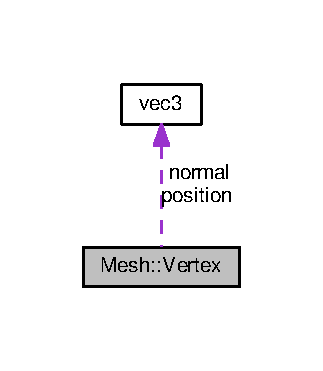
\includegraphics[width=155pt]{structMesh_1_1Vertex__coll__graph}
\end{center}
\end{figure}
\subsection*{Public Attributes}
\begin{DoxyCompactItemize}
\item 
\hyperlink{classvec3}{vec3} \hyperlink{structMesh_1_1Vertex_a6ee1c5ba29f0bf02bf446845de25548f}{position}
\begin{DoxyCompactList}\small\item\em vertex position \end{DoxyCompactList}\item 
\hyperlink{classvec3}{vec3} \hyperlink{structMesh_1_1Vertex_adf43225146648954d9196e4b6fa47379}{normal}
\begin{DoxyCompactList}\small\item\em vertex normal \end{DoxyCompactList}\end{DoxyCompactItemize}


\subsection{Detailed Description}
a vertex consists of a position and a normal 

\subsection{Member Data Documentation}
\index{Mesh\+::\+Vertex@{Mesh\+::\+Vertex}!normal@{normal}}
\index{normal@{normal}!Mesh\+::\+Vertex@{Mesh\+::\+Vertex}}
\subsubsection[{\texorpdfstring{normal}{normal}}]{\setlength{\rightskip}{0pt plus 5cm}{\bf vec3} Mesh\+::\+Vertex\+::normal}\hypertarget{structMesh_1_1Vertex_adf43225146648954d9196e4b6fa47379}{}\label{structMesh_1_1Vertex_adf43225146648954d9196e4b6fa47379}


vertex normal 

\index{Mesh\+::\+Vertex@{Mesh\+::\+Vertex}!position@{position}}
\index{position@{position}!Mesh\+::\+Vertex@{Mesh\+::\+Vertex}}
\subsubsection[{\texorpdfstring{position}{position}}]{\setlength{\rightskip}{0pt plus 5cm}{\bf vec3} Mesh\+::\+Vertex\+::position}\hypertarget{structMesh_1_1Vertex_a6ee1c5ba29f0bf02bf446845de25548f}{}\label{structMesh_1_1Vertex_a6ee1c5ba29f0bf02bf446845de25548f}


vertex position 



The documentation for this struct was generated from the following file\+:\begin{DoxyCompactItemize}
\item 
/home/eason/\+Desktop/assignment\+\_\+0/src/\hyperlink{Mesh_8h}{Mesh.\+h}\end{DoxyCompactItemize}

\chapter{File Documentation}
\hypertarget{README_8md}{}\section{/home/eason/\+Desktop/\+E\+P\+F\+L\+\_\+\+C\+G/assignment\+\_\+3/\+R\+E\+A\+D\+ME.md File Reference}
\label{README_8md}\index{/home/eason/\+Desktop/\+E\+P\+F\+L\+\_\+\+C\+G/assignment\+\_\+3/\+R\+E\+A\+D\+M\+E.\+md@{/home/eason/\+Desktop/\+E\+P\+F\+L\+\_\+\+C\+G/assignment\+\_\+3/\+R\+E\+A\+D\+M\+E.\+md}}

\hypertarget{Camera_8h}{}\section{/home/eason/\+Desktop/\+E\+P\+F\+L\+\_\+\+C\+G/assignment\+\_\+0/src/\+Camera.h File Reference}
\label{Camera_8h}\index{/home/eason/\+Desktop/\+E\+P\+F\+L\+\_\+\+C\+G/assignment\+\_\+0/src/\+Camera.\+h@{/home/eason/\+Desktop/\+E\+P\+F\+L\+\_\+\+C\+G/assignment\+\_\+0/src/\+Camera.\+h}}
{\ttfamily \#include \char`\"{}vec3.\+h\char`\"{}}\\*
Include dependency graph for Camera.\+h\+:

\hypertarget{CMakeLists_8txt}{}\section{/home/eason/\+Desktop/\+E\+P\+F\+L\+\_\+\+C\+G/assignment\+\_\+1/src/\+C\+Make\+Lists.txt File Reference}
\label{CMakeLists_8txt}\index{/home/eason/\+Desktop/\+E\+P\+F\+L\+\_\+\+C\+G/assignment\+\_\+1/src/\+C\+Make\+Lists.\+txt@{/home/eason/\+Desktop/\+E\+P\+F\+L\+\_\+\+C\+G/assignment\+\_\+1/src/\+C\+Make\+Lists.\+txt}}

\hypertarget{Cylinder_8cpp}{}\section{/home/eason/\+Desktop/\+E\+P\+F\+L\+\_\+\+C\+G/assignment\+\_\+2/src/\+Cylinder.cpp File Reference}
\label{Cylinder_8cpp}\index{/home/eason/\+Desktop/\+E\+P\+F\+L\+\_\+\+C\+G/assignment\+\_\+2/src/\+Cylinder.\+cpp@{/home/eason/\+Desktop/\+E\+P\+F\+L\+\_\+\+C\+G/assignment\+\_\+2/src/\+Cylinder.\+cpp}}
{\ttfamily \#include \char`\"{}Cylinder.\+h\char`\"{}}\\*
{\ttfamily \#include \char`\"{}Solve\+Quadratic.\+h\char`\"{}}\\*
{\ttfamily \#include $<$array$>$}\\*
{\ttfamily \#include $<$cmath$>$}\\*
Include dependency graph for Cylinder.\+cpp\+:
% FIG 0

\hypertarget{Cylinder_8h}{}\section{/home/eason/\+Desktop/\+E\+P\+F\+L\+\_\+\+C\+G/assignment\+\_\+0/src/\+Cylinder.h File Reference}
\label{Cylinder_8h}\index{/home/eason/\+Desktop/\+E\+P\+F\+L\+\_\+\+C\+G/assignment\+\_\+0/src/\+Cylinder.\+h@{/home/eason/\+Desktop/\+E\+P\+F\+L\+\_\+\+C\+G/assignment\+\_\+0/src/\+Cylinder.\+h}}
{\ttfamily \#include \char`\"{}Object.\+h\char`\"{}}\\*
{\ttfamily \#include \char`\"{}vec3.\+h\char`\"{}}\\*
Include dependency graph for Cylinder.\+h\+:
% FIG 0
This graph shows which files directly or indirectly include this file\+:
% FIG 1
\subsection*{Classes}
\begin{DoxyCompactItemize}
\item 
class \hyperlink{classCylinder}{Cylinder}
\begin{DoxyCompactList}\small\item\em This class overrides the intersection method \hyperlink{structObject_ac6549d30793a9b3da070234bf10c7e91}{Object\+::intersect()}. \end{DoxyCompactList}\end{DoxyCompactItemize}

\hypertarget{Image_8h}{}\section{/home/eason/\+Desktop/\+E\+P\+F\+L\+\_\+\+C\+G/assignment\+\_\+3/src/\+Image.h File Reference}
\label{Image_8h}\index{/home/eason/\+Desktop/\+E\+P\+F\+L\+\_\+\+C\+G/assignment\+\_\+3/src/\+Image.\+h@{/home/eason/\+Desktop/\+E\+P\+F\+L\+\_\+\+C\+G/assignment\+\_\+3/src/\+Image.\+h}}
{\ttfamily \#include \char`\"{}vec3.\+h\char`\"{}}\\*
{\ttfamily \#include $<$vector$>$}\\*
{\ttfamily \#include $<$assert.\+h$>$}\\*
{\ttfamily \#include $<$fstream$>$}\\*
Include dependency graph for Image.\+h\+:
% FIG 0
This graph shows which files directly or indirectly include this file\+:
% FIG 1
\subsection*{Classes}
\begin{DoxyCompactItemize}
\item 
class \hyperlink{classImage}{Image}
\end{DoxyCompactItemize}

\hypertarget{Light_8h}{}\section{/home/eason/\+Desktop/\+E\+P\+F\+L\+\_\+\+C\+G/assignment\+\_\+3/src/\+Light.h File Reference}
\label{Light_8h}\index{/home/eason/\+Desktop/\+E\+P\+F\+L\+\_\+\+C\+G/assignment\+\_\+3/src/\+Light.\+h@{/home/eason/\+Desktop/\+E\+P\+F\+L\+\_\+\+C\+G/assignment\+\_\+3/src/\+Light.\+h}}
{\ttfamily \#include \char`\"{}vec3.\+h\char`\"{}}\\*
Include dependency graph for Light.\+h\+:
% FIG 0
This graph shows which files directly or indirectly include this file\+:
% FIG 1
\subsection*{Classes}
\begin{DoxyCompactItemize}
\item 
class \hyperlink{structLight}{Light}
\end{DoxyCompactItemize}
\subsection*{Functions}
\begin{DoxyCompactItemize}
\item 
std\+::istream \& \hyperlink{Light_8h_af82e1b3d9a2aa765e246dfbb13b1384d}{operator$>$$>$} (std\+::istream \&is, \hyperlink{structLight}{Light} \&l)
\begin{DoxyCompactList}\small\item\em read light data from stream \end{DoxyCompactList}\end{DoxyCompactItemize}


\subsection{Function Documentation}
\index{Light.\+h@{Light.\+h}!operator$>$$>$@{operator$>$$>$}}
\index{operator$>$$>$@{operator$>$$>$}!Light.\+h@{Light.\+h}}
\subsubsection[{\texorpdfstring{operator$>$$>$(std\+::istream \&is, Light \&l)}{operator>>(std::istream &is, Light &l)}}]{\setlength{\rightskip}{0pt plus 5cm}std\+::istream\& operator$>$$>$ (
\begin{DoxyParamCaption}
\item[{std\+::istream \&}]{is, }
\item[{{\bf Light} \&}]{l}
\end{DoxyParamCaption}
)\hspace{0.3cm}{\ttfamily [inline]}}\hypertarget{Light_8h_af82e1b3d9a2aa765e246dfbb13b1384d}{}\label{Light_8h_af82e1b3d9a2aa765e246dfbb13b1384d}


read light data from stream 


\hypertarget{Material_8h}{}\section{/home/eason/\+Desktop/\+E\+P\+F\+L\+\_\+\+C\+G/assignment\+\_\+3/src/\+Material.h File Reference}
\label{Material_8h}\index{/home/eason/\+Desktop/\+E\+P\+F\+L\+\_\+\+C\+G/assignment\+\_\+3/src/\+Material.\+h@{/home/eason/\+Desktop/\+E\+P\+F\+L\+\_\+\+C\+G/assignment\+\_\+3/src/\+Material.\+h}}
{\ttfamily \#include \char`\"{}vec3.\+h\char`\"{}}\\*
Include dependency graph for Material.\+h\+:
% FIG 0
This graph shows which files directly or indirectly include this file\+:
% FIG 1
\subsection*{Classes}
\begin{DoxyCompactItemize}
\item 
class \hyperlink{structMaterial}{Material}
\end{DoxyCompactItemize}
\subsection*{Functions}
\begin{DoxyCompactItemize}
\item 
std\+::istream \& \hyperlink{Material_8h_a2f9c1e01459b43b47d6aaa72a332836b}{operator$>$$>$} (std\+::istream \&is, \hyperlink{structMaterial}{Material} \&m)
\begin{DoxyCompactList}\small\item\em read material from stream \end{DoxyCompactList}\end{DoxyCompactItemize}


\subsection{Function Documentation}
\index{Material.\+h@{Material.\+h}!operator$>$$>$@{operator$>$$>$}}
\index{operator$>$$>$@{operator$>$$>$}!Material.\+h@{Material.\+h}}
\subsubsection[{\texorpdfstring{operator$>$$>$(std\+::istream \&is, Material \&m)}{operator>>(std::istream &is, Material &m)}}]{\setlength{\rightskip}{0pt plus 5cm}std\+::istream\& operator$>$$>$ (
\begin{DoxyParamCaption}
\item[{std\+::istream \&}]{is, }
\item[{{\bf Material} \&}]{m}
\end{DoxyParamCaption}
)\hspace{0.3cm}{\ttfamily [inline]}}\hypertarget{Material_8h_a2f9c1e01459b43b47d6aaa72a332836b}{}\label{Material_8h_a2f9c1e01459b43b47d6aaa72a332836b}


read material from stream 


\hypertarget{Mesh_8cpp}{}\section{/home/eason/\+Desktop/assignment\+\_\+0/src/\+Mesh.cpp File Reference}
\label{Mesh_8cpp}\index{/home/eason/\+Desktop/assignment\+\_\+0/src/\+Mesh.\+cpp@{/home/eason/\+Desktop/assignment\+\_\+0/src/\+Mesh.\+cpp}}
{\ttfamily \#include \char`\"{}Mesh.\+h\char`\"{}}\\*
{\ttfamily \#include $<$fstream$>$}\\*
{\ttfamily \#include $<$string$>$}\\*
{\ttfamily \#include $<$stdexcept$>$}\\*
{\ttfamily \#include $<$limits$>$}\\*
Include dependency graph for Mesh.\+cpp\+:
\nopagebreak
\begin{figure}[H]
\begin{center}
\leavevmode
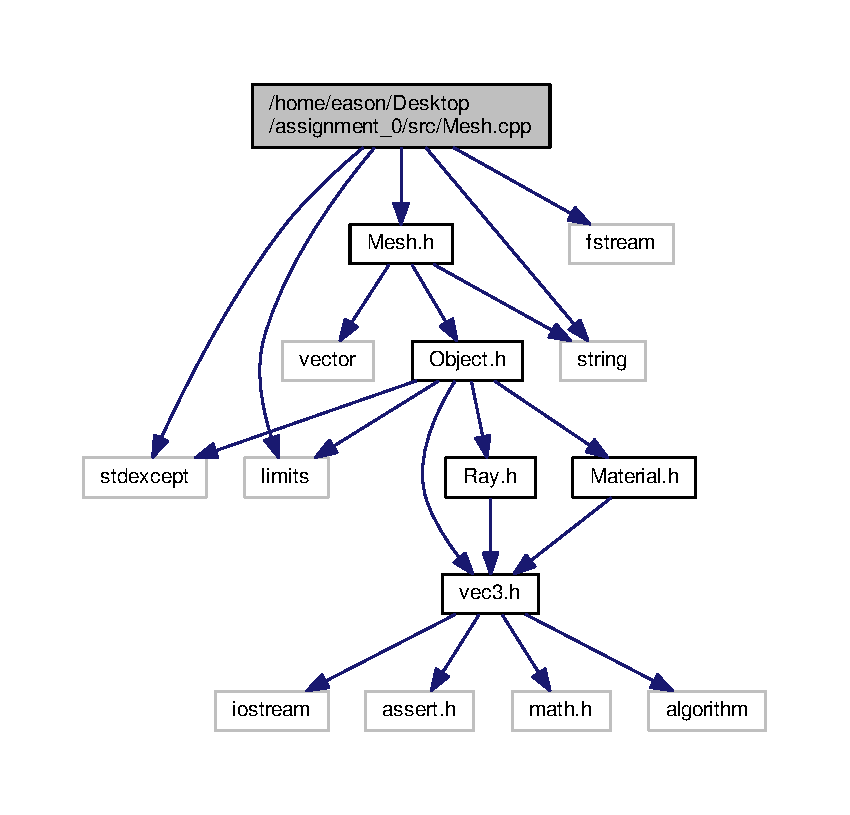
\includegraphics[width=350pt]{Mesh_8cpp__incl}
\end{center}
\end{figure}

\hypertarget{Mesh_8h}{}\section{/home/eason/\+Desktop/\+E\+P\+F\+L\+\_\+\+C\+G/assignment\+\_\+3/src/\+Mesh.h File Reference}
\label{Mesh_8h}\index{/home/eason/\+Desktop/\+E\+P\+F\+L\+\_\+\+C\+G/assignment\+\_\+3/src/\+Mesh.\+h@{/home/eason/\+Desktop/\+E\+P\+F\+L\+\_\+\+C\+G/assignment\+\_\+3/src/\+Mesh.\+h}}
{\ttfamily \#include \char`\"{}Object.\+h\char`\"{}}\\*
{\ttfamily \#include $<$vector$>$}\\*
{\ttfamily \#include $<$string$>$}\\*
Include dependency graph for Mesh.\+h\+:
% FIG 0
This graph shows which files directly or indirectly include this file\+:
% FIG 1
\subsection*{Classes}
\begin{DoxyCompactItemize}
\item 
class \hyperlink{classMesh}{Mesh}
\item 
struct \hyperlink{structMesh_1_1Vertex}{Mesh\+::\+Vertex}
\begin{DoxyCompactList}\small\item\em a vertex consists of a position and a normal \end{DoxyCompactList}\item 
struct \hyperlink{structMesh_1_1Triangle}{Mesh\+::\+Triangle}
\begin{DoxyCompactList}\small\item\em a triangle is specified by three indices and a normal \end{DoxyCompactList}\end{DoxyCompactItemize}

\hypertarget{Object_8h}{}\section{/home/eason/\+Desktop/\+E\+P\+F\+L\+\_\+\+C\+G/assignment\+\_\+0/src/\+Object.h File Reference}
\label{Object_8h}\index{/home/eason/\+Desktop/\+E\+P\+F\+L\+\_\+\+C\+G/assignment\+\_\+0/src/\+Object.\+h@{/home/eason/\+Desktop/\+E\+P\+F\+L\+\_\+\+C\+G/assignment\+\_\+0/src/\+Object.\+h}}
{\ttfamily \#include \char`\"{}Ray.\+h\char`\"{}}\\*
{\ttfamily \#include \char`\"{}vec3.\+h\char`\"{}}\\*
{\ttfamily \#include \char`\"{}Material.\+h\char`\"{}}\\*
{\ttfamily \#include $<$stdexcept$>$}\\*
{\ttfamily \#include $<$limits$>$}\\*
Include dependency graph for Object.\+h\+:
% FIG 0
This graph shows which files directly or indirectly include this file\+:
% FIG 1
\subsection*{Classes}
\begin{DoxyCompactItemize}
\item 
class \hyperlink{structObject}{Object}
\end{DoxyCompactItemize}
\subsection*{Typedefs}
\begin{DoxyCompactItemize}
\item 
typedef \hyperlink{structObject}{Object} $\ast$ \hyperlink{Object_8h_ad537f5b7b240eca7da458a29bbb47b9e}{Object\+\_\+ptr}
\begin{DoxyCompactList}\small\item\em This typedef is for convencience only. \end{DoxyCompactList}\end{DoxyCompactItemize}
\subsection*{Functions}
\begin{DoxyCompactItemize}
\item 
std\+::istream \& \hyperlink{Object_8h_abd08d0da34ef62ea7cc67d55a8aebf46}{operator$>$$>$} (std\+::istream \&is, \hyperlink{structObject}{Object} \&s)
\begin{DoxyCompactList}\small\item\em read object from stream \end{DoxyCompactList}\end{DoxyCompactItemize}


\subsection{Typedef Documentation}
\index{Object.\+h@{Object.\+h}!Object\+\_\+ptr@{Object\+\_\+ptr}}
\index{Object\+\_\+ptr@{Object\+\_\+ptr}!Object.\+h@{Object.\+h}}
\subsubsection[{\texorpdfstring{Object\+\_\+ptr}{Object_ptr}}]{\setlength{\rightskip}{0pt plus 5cm}typedef {\bf Object}$\ast$ {\bf Object\+\_\+ptr}}\hypertarget{Object_8h_ad537f5b7b240eca7da458a29bbb47b9e}{}\label{Object_8h_ad537f5b7b240eca7da458a29bbb47b9e}


This typedef is for convencience only. 



\subsection{Function Documentation}
\index{Object.\+h@{Object.\+h}!operator$>$$>$@{operator$>$$>$}}
\index{operator$>$$>$@{operator$>$$>$}!Object.\+h@{Object.\+h}}
\subsubsection[{\texorpdfstring{operator$>$$>$(std\+::istream \&is, Object \&s)}{operator>>(std::istream &is, Object &s)}}]{\setlength{\rightskip}{0pt plus 5cm}std\+::istream\& operator$>$$>$ (
\begin{DoxyParamCaption}
\item[{std\+::istream \&}]{is, }
\item[{{\bf Object} \&}]{s}
\end{DoxyParamCaption}
)\hspace{0.3cm}{\ttfamily [inline]}}\hypertarget{Object_8h_abd08d0da34ef62ea7cc67d55a8aebf46}{}\label{Object_8h_abd08d0da34ef62ea7cc67d55a8aebf46}


read object from stream 


\hypertarget{Plane_8cpp}{}\section{/home/eason/\+Desktop/assignment\+\_\+0/src/\+Plane.cpp File Reference}
\label{Plane_8cpp}\index{/home/eason/\+Desktop/assignment\+\_\+0/src/\+Plane.\+cpp@{/home/eason/\+Desktop/assignment\+\_\+0/src/\+Plane.\+cpp}}
{\ttfamily \#include \char`\"{}Plane.\+h\char`\"{}}\\*
{\ttfamily \#include $<$limits$>$}\\*
Include dependency graph for Plane.\+cpp\+:
\nopagebreak
\begin{figure}[H]
\begin{center}
\leavevmode
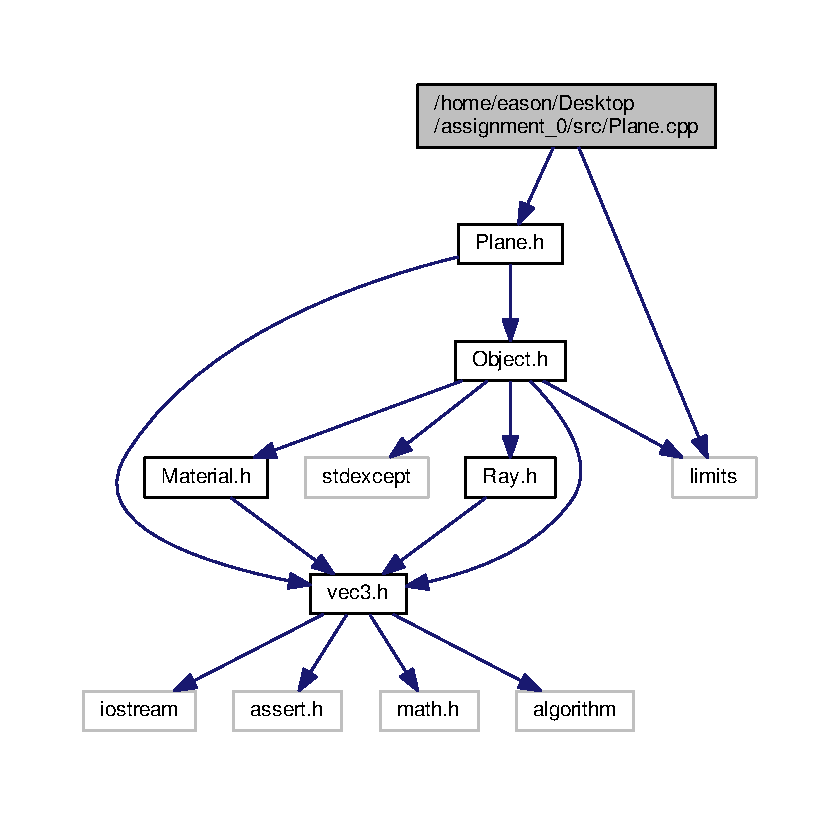
\includegraphics[width=350pt]{Plane_8cpp__incl}
\end{center}
\end{figure}

\hypertarget{Plane_8h}{}\section{/home/eason/\+Desktop/\+E\+P\+F\+L\+\_\+\+C\+G/assignment\+\_\+1/src/\+Plane.h File Reference}
\label{Plane_8h}\index{/home/eason/\+Desktop/\+E\+P\+F\+L\+\_\+\+C\+G/assignment\+\_\+1/src/\+Plane.\+h@{/home/eason/\+Desktop/\+E\+P\+F\+L\+\_\+\+C\+G/assignment\+\_\+1/src/\+Plane.\+h}}
{\ttfamily \#include \char`\"{}Object.\+h\char`\"{}}\\*
{\ttfamily \#include \char`\"{}vec3.\+h\char`\"{}}\\*
Include dependency graph for Plane.\+h\+:
% FIG 0
This graph shows which files directly or indirectly include this file\+:
% FIG 1
\subsection*{Classes}
\begin{DoxyCompactItemize}
\item 
class \hyperlink{classPlane}{Plane}
\end{DoxyCompactItemize}

\hypertarget{Ray_8h}{}\section{/home/eason/\+Desktop/\+E\+P\+F\+L\+\_\+\+C\+G/assignment\+\_\+0/src/\+Ray.h File Reference}
\label{Ray_8h}\index{/home/eason/\+Desktop/\+E\+P\+F\+L\+\_\+\+C\+G/assignment\+\_\+0/src/\+Ray.\+h@{/home/eason/\+Desktop/\+E\+P\+F\+L\+\_\+\+C\+G/assignment\+\_\+0/src/\+Ray.\+h}}
{\ttfamily \#include \char`\"{}vec3.\+h\char`\"{}}\\*
Include dependency graph for Ray.\+h\+:
% FIG 0
This graph shows which files directly or indirectly include this file\+:
% FIG 1
\subsection*{Classes}
\begin{DoxyCompactItemize}
\item 
class \hyperlink{classRay}{Ray}
\end{DoxyCompactItemize}
\subsection*{Functions}
\begin{DoxyCompactItemize}
\item 
std\+::istream \& \hyperlink{Ray_8h_a8db39a6528a9176f01b285b4b3886c7a}{operator$>$$>$} (std\+::istream \&is, \hyperlink{classRay}{Ray} \&r)
\begin{DoxyCompactList}\small\item\em read ray from stream \end{DoxyCompactList}\end{DoxyCompactItemize}


\subsection{Function Documentation}
\index{Ray.\+h@{Ray.\+h}!operator$>$$>$@{operator$>$$>$}}
\index{operator$>$$>$@{operator$>$$>$}!Ray.\+h@{Ray.\+h}}
\subsubsection[{\texorpdfstring{operator$>$$>$(std\+::istream \&is, Ray \&r)}{operator>>(std::istream &is, Ray &r)}}]{\setlength{\rightskip}{0pt plus 5cm}std\+::istream\& operator$>$$>$ (
\begin{DoxyParamCaption}
\item[{std\+::istream \&}]{is, }
\item[{{\bf Ray} \&}]{r}
\end{DoxyParamCaption}
)\hspace{0.3cm}{\ttfamily [inline]}}\hypertarget{Ray_8h_a8db39a6528a9176f01b285b4b3886c7a}{}\label{Ray_8h_a8db39a6528a9176f01b285b4b3886c7a}


read ray from stream 


\hypertarget{raytrace_8cpp}{}\section{/home/eason/\+Desktop/assignment\+\_\+0/src/raytrace.cpp File Reference}
\label{raytrace_8cpp}\index{/home/eason/\+Desktop/assignment\+\_\+0/src/raytrace.\+cpp@{/home/eason/\+Desktop/assignment\+\_\+0/src/raytrace.\+cpp}}
{\ttfamily \#include \char`\"{}Stop\+Watch.\+h\char`\"{}}\\*
{\ttfamily \#include \char`\"{}Scene.\+h\char`\"{}}\\*
{\ttfamily \#include $<$vector$>$}\\*
{\ttfamily \#include $<$iostream$>$}\\*
{\ttfamily \#include $<$string$>$}\\*
{\ttfamily \#include $<$fstream$>$}\\*
Include dependency graph for raytrace.\+cpp\+:
\nopagebreak
\begin{figure}[H]
\begin{center}
\leavevmode
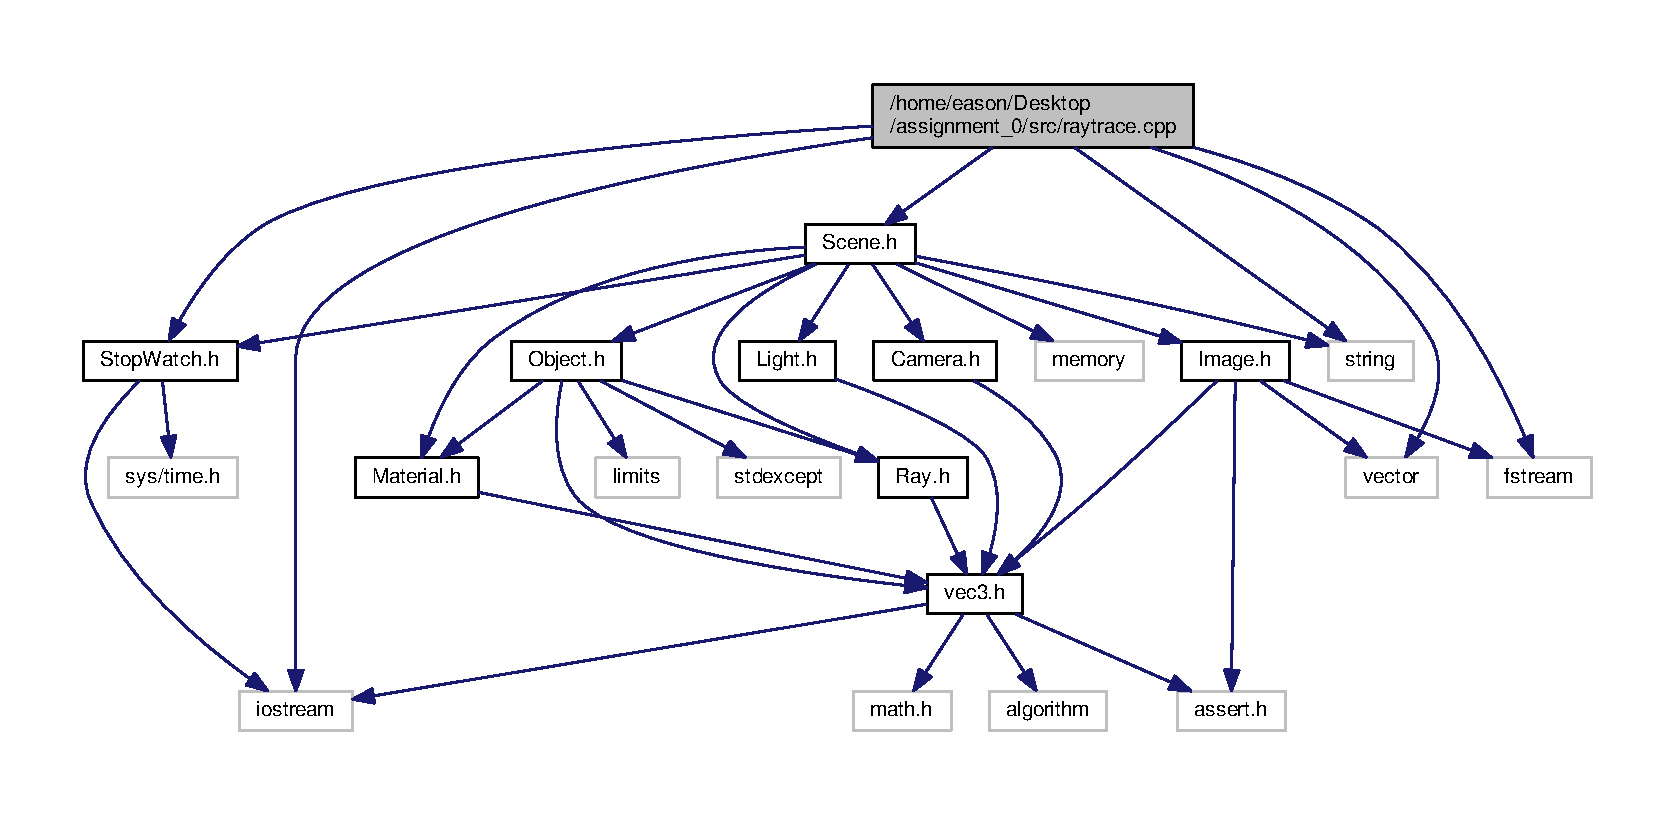
\includegraphics[width=350pt]{raytrace_8cpp__incl}
\end{center}
\end{figure}
\subsection*{Functions}
\begin{DoxyCompactItemize}
\item 
int \hyperlink{raytrace_8cpp_a3c04138a5bfe5d72780bb7e82a18e627}{main} (int argc, char $\ast$$\ast$argv)
\begin{DoxyCompactList}\small\item\em Program entry point. \end{DoxyCompactList}\end{DoxyCompactItemize}


\subsection{Function Documentation}
\index{raytrace.\+cpp@{raytrace.\+cpp}!main@{main}}
\index{main@{main}!raytrace.\+cpp@{raytrace.\+cpp}}
\subsubsection[{\texorpdfstring{main(int argc, char $\ast$$\ast$argv)}{main(int argc, char **argv)}}]{\setlength{\rightskip}{0pt plus 5cm}int main (
\begin{DoxyParamCaption}
\item[{int}]{argc, }
\item[{char $\ast$$\ast$}]{argv}
\end{DoxyParamCaption}
)}\hypertarget{raytrace_8cpp_a3c04138a5bfe5d72780bb7e82a18e627}{}\label{raytrace_8cpp_a3c04138a5bfe5d72780bb7e82a18e627}


Program entry point. 


\hypertarget{Scene_8cpp}{}\section{/home/eason/\+Desktop/assignment\+\_\+0/src/\+Scene.cpp File Reference}
\label{Scene_8cpp}\index{/home/eason/\+Desktop/assignment\+\_\+0/src/\+Scene.\+cpp@{/home/eason/\+Desktop/assignment\+\_\+0/src/\+Scene.\+cpp}}
{\ttfamily \#include \char`\"{}Scene.\+h\char`\"{}}\\*
{\ttfamily \#include \char`\"{}Plane.\+h\char`\"{}}\\*
{\ttfamily \#include \char`\"{}Sphere.\+h\char`\"{}}\\*
{\ttfamily \#include \char`\"{}Cylinder.\+h\char`\"{}}\\*
{\ttfamily \#include \char`\"{}Mesh.\+h\char`\"{}}\\*
{\ttfamily \#include $<$limits$>$}\\*
{\ttfamily \#include $<$map$>$}\\*
{\ttfamily \#include $<$functional$>$}\\*
{\ttfamily \#include $<$stdexcept$>$}\\*
Include dependency graph for Scene.\+cpp\+:
\nopagebreak
\begin{figure}[H]
\begin{center}
\leavevmode
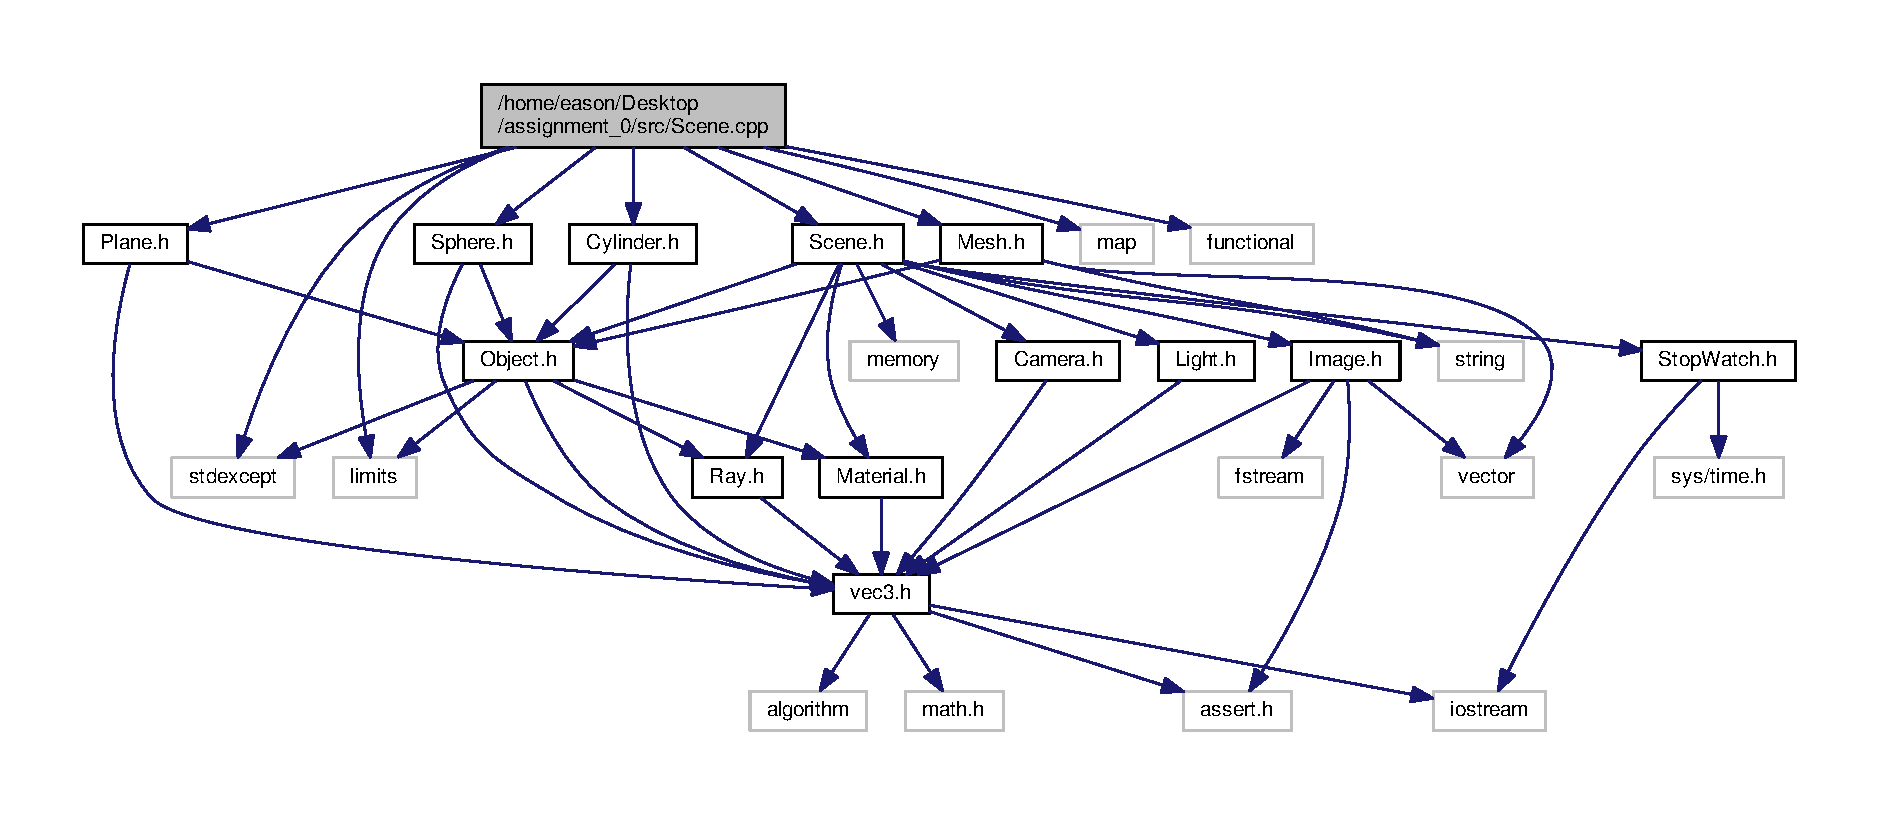
\includegraphics[width=350pt]{Scene_8cpp__incl}
\end{center}
\end{figure}

\hypertarget{Scene_8h}{}\section{/home/eason/\+Desktop/\+E\+P\+F\+L\+\_\+\+C\+G/assignment\+\_\+3/src/\+Scene.h File Reference}
\label{Scene_8h}\index{/home/eason/\+Desktop/\+E\+P\+F\+L\+\_\+\+C\+G/assignment\+\_\+3/src/\+Scene.\+h@{/home/eason/\+Desktop/\+E\+P\+F\+L\+\_\+\+C\+G/assignment\+\_\+3/src/\+Scene.\+h}}
{\ttfamily \#include \char`\"{}Stop\+Watch.\+h\char`\"{}}\\*
{\ttfamily \#include \char`\"{}Object.\+h\char`\"{}}\\*
{\ttfamily \#include \char`\"{}Light.\+h\char`\"{}}\\*
{\ttfamily \#include \char`\"{}Ray.\+h\char`\"{}}\\*
{\ttfamily \#include \char`\"{}Material.\+h\char`\"{}}\\*
{\ttfamily \#include \char`\"{}Image.\+h\char`\"{}}\\*
{\ttfamily \#include \char`\"{}Camera.\+h\char`\"{}}\\*
{\ttfamily \#include $<$memory$>$}\\*
{\ttfamily \#include $<$string$>$}\\*
Include dependency graph for Scene.\+h\+:
% FIG 0
This graph shows which files directly or indirectly include this file\+:
% FIG 1
\subsection*{Classes}
\begin{DoxyCompactItemize}
\item 
class \hyperlink{classScene}{Scene}
\end{DoxyCompactItemize}

\hypertarget{SolveQuadratic_8h}{}\section{/home/eason/\+Desktop/\+E\+P\+F\+L\+\_\+\+C\+G/assignment\+\_\+2/src/\+Solve\+Quadratic.h File Reference}
\label{SolveQuadratic_8h}\index{/home/eason/\+Desktop/\+E\+P\+F\+L\+\_\+\+C\+G/assignment\+\_\+2/src/\+Solve\+Quadratic.\+h@{/home/eason/\+Desktop/\+E\+P\+F\+L\+\_\+\+C\+G/assignment\+\_\+2/src/\+Solve\+Quadratic.\+h}}
{\ttfamily \#include $<$cmath$>$}\\*
{\ttfamily \#include $<$array$>$}\\*
Include dependency graph for Solve\+Quadratic.\+h\+:
% FIG 0
This graph shows which files directly or indirectly include this file\+:
% FIG 1
\subsection*{Functions}
\begin{DoxyCompactItemize}
\item 
size\+\_\+t \hyperlink{SolveQuadratic_8h_a019e16c4c818ad33bbaed94fee0ec01e}{solve\+Quadratic} (double a, double b, double c, std\+::array$<$ double, 2 $>$ \&solns)
\end{DoxyCompactItemize}


\subsection{Function Documentation}
\index{Solve\+Quadratic.\+h@{Solve\+Quadratic.\+h}!solve\+Quadratic@{solve\+Quadratic}}
\index{solve\+Quadratic@{solve\+Quadratic}!Solve\+Quadratic.\+h@{Solve\+Quadratic.\+h}}
\subsubsection[{\texorpdfstring{solve\+Quadratic(double a, double b, double c, std\+::array$<$ double, 2 $>$ \&solns)}{solveQuadratic(double a, double b, double c, std::array< double, 2 > &solns)}}]{\setlength{\rightskip}{0pt plus 5cm}size\+\_\+t solve\+Quadratic (
\begin{DoxyParamCaption}
\item[{double}]{a, }
\item[{double}]{b, }
\item[{double}]{c, }
\item[{std\+::array$<$ double, 2 $>$ \&}]{solns}
\end{DoxyParamCaption}
)\hspace{0.3cm}{\ttfamily [inline]}}\hypertarget{SolveQuadratic_8h_a019e16c4c818ad33bbaed94fee0ec01e}{}\label{SolveQuadratic_8h_a019e16c4c818ad33bbaed94fee0ec01e}
Numerically robust solution to (possibly degenerate) quadratic equations. Avoids catastrophic cancellation and handles equations that have degenerated to become linear or constant. 
\begin{DoxyParams}[1]{Parameters}
\mbox{\tt in}  & {\em a,b,c} & coefficients of ax$^\wedge$2 + bx + c == 0 \\
\hline
\mbox{\tt out}  & {\em solns} & array holding between 0 and 2 solutions \\
\hline
\end{DoxyParams}
\begin{DoxyReturn}{Returns}
number of solutions found 
\end{DoxyReturn}

\hypertarget{Sphere_8cpp}{}\section{/home/eason/\+Desktop/\+E\+P\+F\+L\+\_\+\+C\+G/assignment\+\_\+2/src/\+Sphere.cpp File Reference}
\label{Sphere_8cpp}\index{/home/eason/\+Desktop/\+E\+P\+F\+L\+\_\+\+C\+G/assignment\+\_\+2/src/\+Sphere.\+cpp@{/home/eason/\+Desktop/\+E\+P\+F\+L\+\_\+\+C\+G/assignment\+\_\+2/src/\+Sphere.\+cpp}}
{\ttfamily \#include \char`\"{}Sphere.\+h\char`\"{}}\\*
{\ttfamily \#include \char`\"{}Solve\+Quadratic.\+h\char`\"{}}\\*
Include dependency graph for Sphere.\+cpp\+:
% FIG 0

\hypertarget{Sphere_8h}{}\section{/home/eason/\+Desktop/\+E\+P\+F\+L\+\_\+\+C\+G/assignment\+\_\+3/src/\+Sphere.h File Reference}
\label{Sphere_8h}\index{/home/eason/\+Desktop/\+E\+P\+F\+L\+\_\+\+C\+G/assignment\+\_\+3/src/\+Sphere.\+h@{/home/eason/\+Desktop/\+E\+P\+F\+L\+\_\+\+C\+G/assignment\+\_\+3/src/\+Sphere.\+h}}
{\ttfamily \#include \char`\"{}Object.\+h\char`\"{}}\\*
{\ttfamily \#include \char`\"{}vec3.\+h\char`\"{}}\\*
Include dependency graph for Sphere.\+h\+:
% FIG 0
This graph shows which files directly or indirectly include this file\+:
% FIG 1
\subsection*{Classes}
\begin{DoxyCompactItemize}
\item 
class \hyperlink{classSphere}{Sphere}
\end{DoxyCompactItemize}

\hypertarget{StopWatch_8h}{}\section{/home/eason/\+Desktop/\+E\+P\+F\+L\+\_\+\+C\+G/assignment\+\_\+2/src/\+Stop\+Watch.h File Reference}
\label{StopWatch_8h}\index{/home/eason/\+Desktop/\+E\+P\+F\+L\+\_\+\+C\+G/assignment\+\_\+2/src/\+Stop\+Watch.\+h@{/home/eason/\+Desktop/\+E\+P\+F\+L\+\_\+\+C\+G/assignment\+\_\+2/src/\+Stop\+Watch.\+h}}
{\ttfamily \#include $<$sys/time.\+h$>$}\\*
{\ttfamily \#include $<$iostream$>$}\\*
Include dependency graph for Stop\+Watch.\+h\+:
% FIG 0
This graph shows which files directly or indirectly include this file\+:
% FIG 1
\subsection*{Classes}
\begin{DoxyCompactItemize}
\item 
class \hyperlink{classStopWatch}{Stop\+Watch}
\end{DoxyCompactItemize}
\subsection*{Functions}
\begin{DoxyCompactItemize}
\item 
std\+::ostream \& \hyperlink{StopWatch_8h_afc3a897ea48e4561c117fccd9448b6b1}{operator$<$$<$} (std\+::ostream \&\+\_\+os, const \hyperlink{classStopWatch}{Stop\+Watch} \&\+\_\+timer)
\begin{DoxyCompactList}\small\item\em output a timer to a stream \end{DoxyCompactList}\end{DoxyCompactItemize}


\subsection{Function Documentation}
\index{Stop\+Watch.\+h@{Stop\+Watch.\+h}!operator$<$$<$@{operator$<$$<$}}
\index{operator$<$$<$@{operator$<$$<$}!Stop\+Watch.\+h@{Stop\+Watch.\+h}}
\subsubsection[{\texorpdfstring{operator$<$$<$(std\+::ostream \&\+\_\+os, const Stop\+Watch \&\+\_\+timer)}{operator<<(std::ostream &_os, const StopWatch &_timer)}}]{\setlength{\rightskip}{0pt plus 5cm}std\+::ostream\& operator$<$$<$ (
\begin{DoxyParamCaption}
\item[{std\+::ostream \&}]{\+\_\+os, }
\item[{const {\bf Stop\+Watch} \&}]{\+\_\+timer}
\end{DoxyParamCaption}
)\hspace{0.3cm}{\ttfamily [inline]}}\hypertarget{StopWatch_8h_afc3a897ea48e4561c117fccd9448b6b1}{}\label{StopWatch_8h_afc3a897ea48e4561c117fccd9448b6b1}


output a timer to a stream 


\hypertarget{vec3_8cpp}{}\section{/home/eason/\+Desktop/\+E\+P\+F\+L\+\_\+\+C\+G/assignment\+\_\+3/src/vec3.cpp File Reference}
\label{vec3_8cpp}\index{/home/eason/\+Desktop/\+E\+P\+F\+L\+\_\+\+C\+G/assignment\+\_\+3/src/vec3.\+cpp@{/home/eason/\+Desktop/\+E\+P\+F\+L\+\_\+\+C\+G/assignment\+\_\+3/src/vec3.\+cpp}}
{\ttfamily \#include \char`\"{}vec3.\+h\char`\"{}}\\*
Include dependency graph for vec3.\+cpp\+:
% FIG 0

\hypertarget{vec3_8h}{}\section{/home/eason/\+Desktop/\+E\+P\+F\+L\+\_\+\+C\+G/assignment\+\_\+1/src/vec3.h File Reference}
\label{vec3_8h}\index{/home/eason/\+Desktop/\+E\+P\+F\+L\+\_\+\+C\+G/assignment\+\_\+1/src/vec3.\+h@{/home/eason/\+Desktop/\+E\+P\+F\+L\+\_\+\+C\+G/assignment\+\_\+1/src/vec3.\+h}}


Implements the vector class and its mathematical operations.  


{\ttfamily \#include $<$iostream$>$}\\*
{\ttfamily \#include $<$assert.\+h$>$}\\*
{\ttfamily \#include $<$math.\+h$>$}\\*
{\ttfamily \#include $<$algorithm$>$}\\*
Include dependency graph for vec3.\+h\+:
% FIG 0
This graph shows which files directly or indirectly include this file\+:
% FIG 1
\subsection*{Classes}
\begin{DoxyCompactItemize}
\item 
class \hyperlink{classvec3}{vec3}
\end{DoxyCompactItemize}
\subsection*{Functions}
\begin{DoxyCompactItemize}
\item 
const \hyperlink{classvec3}{vec3} \hyperlink{vec3_8h_aadaf3215f08daa75822dba381804233d}{operator-\/} (const \hyperlink{classvec3}{vec3} \&v)
\begin{DoxyCompactList}\small\item\em unary minus\+: turn v into -\/v \end{DoxyCompactList}\item 
const \hyperlink{classvec3}{vec3} \hyperlink{vec3_8h_aa4f93e60ec26c63f5f5f69107e9fa208}{operator$\ast$} (const double s, const \hyperlink{classvec3}{vec3} \&v)
\begin{DoxyCompactList}\small\item\em multiply vector {\ttfamily v} by scalar {\ttfamily s} \end{DoxyCompactList}\item 
const \hyperlink{classvec3}{vec3} \hyperlink{vec3_8h_a57beb01e5a7126e742cb2f5d77f20a8d}{operator$\ast$} (const \hyperlink{classvec3}{vec3} \&v, const double s)
\begin{DoxyCompactList}\small\item\em multiply vector {\ttfamily v} by scalar {\ttfamily s} \end{DoxyCompactList}\item 
const \hyperlink{classvec3}{vec3} \hyperlink{vec3_8h_af444fe3c8a058ed1736d9679d42bd84b}{operator$\ast$} (const \hyperlink{classvec3}{vec3} \&v0, const \hyperlink{classvec3}{vec3} \&v1)
\begin{DoxyCompactList}\small\item\em component-\/wise multiplication of vectors {\ttfamily v0} and {\ttfamily v1} \end{DoxyCompactList}\item 
const \hyperlink{classvec3}{vec3} \hyperlink{vec3_8h_a0272bbe6135b89ae2a378e03ff809d4b}{operator/} (const \hyperlink{classvec3}{vec3} \&v, const double s)
\begin{DoxyCompactList}\small\item\em divide vector {\ttfamily v} by scalar {\ttfamily s} \end{DoxyCompactList}\item 
const \hyperlink{classvec3}{vec3} \hyperlink{vec3_8h_a2bd9ca78c7ca8be54afc9500ff89117d}{operator+} (const \hyperlink{classvec3}{vec3} \&v0, const \hyperlink{classvec3}{vec3} \&v1)
\begin{DoxyCompactList}\small\item\em add two vectors {\ttfamily v0} and {\ttfamily v1} \end{DoxyCompactList}\item 
const \hyperlink{classvec3}{vec3} \hyperlink{vec3_8h_aa8cf6ba584300aeb08b9d9143635680a}{operator-\/} (const \hyperlink{classvec3}{vec3} \&v0, const \hyperlink{classvec3}{vec3} \&v1)
\begin{DoxyCompactList}\small\item\em subtract vector {\ttfamily v1} from vector {\ttfamily v0} \end{DoxyCompactList}\item 
const \hyperlink{classvec3}{vec3} \hyperlink{vec3_8h_ab7afd8764c8e083204e00a6e7695d052}{min} (const \hyperlink{classvec3}{vec3} \&v0, const \hyperlink{classvec3}{vec3} \&v1)
\begin{DoxyCompactList}\small\item\em compute the component-\/wise minimum of vectors {\ttfamily v0} and {\ttfamily v1} \end{DoxyCompactList}\item 
const \hyperlink{classvec3}{vec3} \hyperlink{vec3_8h_a88bf317d8d46ef981cc71e72eb77b184}{max} (const \hyperlink{classvec3}{vec3} \&v0, const \hyperlink{classvec3}{vec3} \&v1)
\begin{DoxyCompactList}\small\item\em compute the component-\/wise maximum of vectors {\ttfamily v0} and {\ttfamily v1} \end{DoxyCompactList}\item 
const double \hyperlink{vec3_8h_ae151aaaf178ce355329547d9abd97089}{dot} (const \hyperlink{classvec3}{vec3} \&v0, const \hyperlink{classvec3}{vec3} \&v1)
\begin{DoxyCompactList}\small\item\em compute the Euclidean dot product of {\ttfamily v0} and {\ttfamily v1} \end{DoxyCompactList}\item 
const double \hyperlink{vec3_8h_ab3f6a10e697cc19b6487a8d13c30cb6d}{norm} (const \hyperlink{classvec3}{vec3} \&v)
\begin{DoxyCompactList}\small\item\em compute the Euclidean norm (length) of a vector {\ttfamily v} \end{DoxyCompactList}\item 
const \hyperlink{classvec3}{vec3} \hyperlink{vec3_8h_a541c1fc23b130b6a2004c90901505f14}{normalize} (const \hyperlink{classvec3}{vec3} \&v)
\begin{DoxyCompactList}\small\item\em normalize vector {\ttfamily v} by dividing it by its norm \end{DoxyCompactList}\item 
const double \hyperlink{vec3_8h_a8ce1797e44c9afb838b7aa28a93b4db7}{distance} (const \hyperlink{classvec3}{vec3} \&v0, const \hyperlink{classvec3}{vec3} \&v1)
\begin{DoxyCompactList}\small\item\em compute the distance between vectors {\ttfamily v0} and {\ttfamily v1} \end{DoxyCompactList}\item 
const \hyperlink{classvec3}{vec3} \hyperlink{vec3_8h_a300b47ffa1833ec786fc2f49da86ac4a}{cross} (const \hyperlink{classvec3}{vec3} \&v0, const \hyperlink{classvec3}{vec3} \&v1)
\begin{DoxyCompactList}\small\item\em compute the cross product of {\ttfamily v0} and {\ttfamily v1} \end{DoxyCompactList}\item 
const \hyperlink{classvec3}{vec3} \hyperlink{vec3_8h_a35b64cc9ea1af33a921da839d3349645}{reflect} (const \hyperlink{classvec3}{vec3} \&v, const \hyperlink{classvec3}{vec3} \&n)
\begin{DoxyCompactList}\small\item\em reflect vector {\ttfamily v} at normal {\ttfamily n} \end{DoxyCompactList}\item 
const \hyperlink{classvec3}{vec3} \hyperlink{vec3_8h_a8dc27d741a8c2be5d12953c024b65521}{mirror} (const \hyperlink{classvec3}{vec3} \&v, const \hyperlink{classvec3}{vec3} \&n)
\begin{DoxyCompactList}\small\item\em mirrors vector {\ttfamily v} at normal {\ttfamily n} \end{DoxyCompactList}\item 
std\+::istream \& \hyperlink{vec3_8h_ab705d3337286a4262e84bbbb0b694a56}{operator$>$$>$} (std\+::istream \&is, \hyperlink{classvec3}{vec3} \&v)
\begin{DoxyCompactList}\small\item\em read the space-\/separated components of a vector from a stream \end{DoxyCompactList}\item 
std\+::ostream \& \hyperlink{vec3_8h_a3e8f4856b29a4320f185f9a9cf0f94bc}{operator$<$$<$} (std\+::ostream \&os, const \hyperlink{classvec3}{vec3} \&v)
\begin{DoxyCompactList}\small\item\em output a vector by printing its comma-\/separated compontens \end{DoxyCompactList}\end{DoxyCompactItemize}


\subsection{Detailed Description}
Implements the vector class and its mathematical operations. 



\subsection{Function Documentation}
\index{vec3.\+h@{vec3.\+h}!cross@{cross}}
\index{cross@{cross}!vec3.\+h@{vec3.\+h}}
\subsubsection[{\texorpdfstring{cross(const vec3 \&v0, const vec3 \&v1)}{cross(const vec3 &v0, const vec3 &v1)}}]{\setlength{\rightskip}{0pt plus 5cm}const {\bf vec3} cross (
\begin{DoxyParamCaption}
\item[{const {\bf vec3} \&}]{v0, }
\item[{const {\bf vec3} \&}]{v1}
\end{DoxyParamCaption}
)\hspace{0.3cm}{\ttfamily [inline]}}\hypertarget{vec3_8h_a300b47ffa1833ec786fc2f49da86ac4a}{}\label{vec3_8h_a300b47ffa1833ec786fc2f49da86ac4a}


compute the cross product of {\ttfamily v0} and {\ttfamily v1} 

\index{vec3.\+h@{vec3.\+h}!distance@{distance}}
\index{distance@{distance}!vec3.\+h@{vec3.\+h}}
\subsubsection[{\texorpdfstring{distance(const vec3 \&v0, const vec3 \&v1)}{distance(const vec3 &v0, const vec3 &v1)}}]{\setlength{\rightskip}{0pt plus 5cm}const double distance (
\begin{DoxyParamCaption}
\item[{const {\bf vec3} \&}]{v0, }
\item[{const {\bf vec3} \&}]{v1}
\end{DoxyParamCaption}
)\hspace{0.3cm}{\ttfamily [inline]}}\hypertarget{vec3_8h_a8ce1797e44c9afb838b7aa28a93b4db7}{}\label{vec3_8h_a8ce1797e44c9afb838b7aa28a93b4db7}


compute the distance between vectors {\ttfamily v0} and {\ttfamily v1} 

\index{vec3.\+h@{vec3.\+h}!dot@{dot}}
\index{dot@{dot}!vec3.\+h@{vec3.\+h}}
\subsubsection[{\texorpdfstring{dot(const vec3 \&v0, const vec3 \&v1)}{dot(const vec3 &v0, const vec3 &v1)}}]{\setlength{\rightskip}{0pt plus 5cm}const double dot (
\begin{DoxyParamCaption}
\item[{const {\bf vec3} \&}]{v0, }
\item[{const {\bf vec3} \&}]{v1}
\end{DoxyParamCaption}
)\hspace{0.3cm}{\ttfamily [inline]}}\hypertarget{vec3_8h_ae151aaaf178ce355329547d9abd97089}{}\label{vec3_8h_ae151aaaf178ce355329547d9abd97089}


compute the Euclidean dot product of {\ttfamily v0} and {\ttfamily v1} 

\index{vec3.\+h@{vec3.\+h}!max@{max}}
\index{max@{max}!vec3.\+h@{vec3.\+h}}
\subsubsection[{\texorpdfstring{max(const vec3 \&v0, const vec3 \&v1)}{max(const vec3 &v0, const vec3 &v1)}}]{\setlength{\rightskip}{0pt plus 5cm}const {\bf vec3} max (
\begin{DoxyParamCaption}
\item[{const {\bf vec3} \&}]{v0, }
\item[{const {\bf vec3} \&}]{v1}
\end{DoxyParamCaption}
)\hspace{0.3cm}{\ttfamily [inline]}}\hypertarget{vec3_8h_a88bf317d8d46ef981cc71e72eb77b184}{}\label{vec3_8h_a88bf317d8d46ef981cc71e72eb77b184}


compute the component-\/wise maximum of vectors {\ttfamily v0} and {\ttfamily v1} 

\index{vec3.\+h@{vec3.\+h}!min@{min}}
\index{min@{min}!vec3.\+h@{vec3.\+h}}
\subsubsection[{\texorpdfstring{min(const vec3 \&v0, const vec3 \&v1)}{min(const vec3 &v0, const vec3 &v1)}}]{\setlength{\rightskip}{0pt plus 5cm}const {\bf vec3} min (
\begin{DoxyParamCaption}
\item[{const {\bf vec3} \&}]{v0, }
\item[{const {\bf vec3} \&}]{v1}
\end{DoxyParamCaption}
)\hspace{0.3cm}{\ttfamily [inline]}}\hypertarget{vec3_8h_ab7afd8764c8e083204e00a6e7695d052}{}\label{vec3_8h_ab7afd8764c8e083204e00a6e7695d052}


compute the component-\/wise minimum of vectors {\ttfamily v0} and {\ttfamily v1} 

\index{vec3.\+h@{vec3.\+h}!mirror@{mirror}}
\index{mirror@{mirror}!vec3.\+h@{vec3.\+h}}
\subsubsection[{\texorpdfstring{mirror(const vec3 \&v, const vec3 \&n)}{mirror(const vec3 &v, const vec3 &n)}}]{\setlength{\rightskip}{0pt plus 5cm}const {\bf vec3} mirror (
\begin{DoxyParamCaption}
\item[{const {\bf vec3} \&}]{v, }
\item[{const {\bf vec3} \&}]{n}
\end{DoxyParamCaption}
)\hspace{0.3cm}{\ttfamily [inline]}}\hypertarget{vec3_8h_a8dc27d741a8c2be5d12953c024b65521}{}\label{vec3_8h_a8dc27d741a8c2be5d12953c024b65521}


mirrors vector {\ttfamily v} at normal {\ttfamily n} 

\index{vec3.\+h@{vec3.\+h}!norm@{norm}}
\index{norm@{norm}!vec3.\+h@{vec3.\+h}}
\subsubsection[{\texorpdfstring{norm(const vec3 \&v)}{norm(const vec3 &v)}}]{\setlength{\rightskip}{0pt plus 5cm}const double norm (
\begin{DoxyParamCaption}
\item[{const {\bf vec3} \&}]{v}
\end{DoxyParamCaption}
)\hspace{0.3cm}{\ttfamily [inline]}}\hypertarget{vec3_8h_ab3f6a10e697cc19b6487a8d13c30cb6d}{}\label{vec3_8h_ab3f6a10e697cc19b6487a8d13c30cb6d}


compute the Euclidean norm (length) of a vector {\ttfamily v} 

\index{vec3.\+h@{vec3.\+h}!normalize@{normalize}}
\index{normalize@{normalize}!vec3.\+h@{vec3.\+h}}
\subsubsection[{\texorpdfstring{normalize(const vec3 \&v)}{normalize(const vec3 &v)}}]{\setlength{\rightskip}{0pt plus 5cm}const {\bf vec3} normalize (
\begin{DoxyParamCaption}
\item[{const {\bf vec3} \&}]{v}
\end{DoxyParamCaption}
)\hspace{0.3cm}{\ttfamily [inline]}}\hypertarget{vec3_8h_a541c1fc23b130b6a2004c90901505f14}{}\label{vec3_8h_a541c1fc23b130b6a2004c90901505f14}


normalize vector {\ttfamily v} by dividing it by its norm 

\index{vec3.\+h@{vec3.\+h}!operator$\ast$@{operator$\ast$}}
\index{operator$\ast$@{operator$\ast$}!vec3.\+h@{vec3.\+h}}
\subsubsection[{\texorpdfstring{operator$\ast$(const double s, const vec3 \&v)}{operator*(const double s, const vec3 &v)}}]{\setlength{\rightskip}{0pt plus 5cm}const {\bf vec3} operator$\ast$ (
\begin{DoxyParamCaption}
\item[{const double}]{s, }
\item[{const {\bf vec3} \&}]{v}
\end{DoxyParamCaption}
)\hspace{0.3cm}{\ttfamily [inline]}}\hypertarget{vec3_8h_aa4f93e60ec26c63f5f5f69107e9fa208}{}\label{vec3_8h_aa4f93e60ec26c63f5f5f69107e9fa208}


multiply vector {\ttfamily v} by scalar {\ttfamily s} 

\index{vec3.\+h@{vec3.\+h}!operator$\ast$@{operator$\ast$}}
\index{operator$\ast$@{operator$\ast$}!vec3.\+h@{vec3.\+h}}
\subsubsection[{\texorpdfstring{operator$\ast$(const vec3 \&v, const double s)}{operator*(const vec3 &v, const double s)}}]{\setlength{\rightskip}{0pt plus 5cm}const {\bf vec3} operator$\ast$ (
\begin{DoxyParamCaption}
\item[{const {\bf vec3} \&}]{v, }
\item[{const double}]{s}
\end{DoxyParamCaption}
)\hspace{0.3cm}{\ttfamily [inline]}}\hypertarget{vec3_8h_a57beb01e5a7126e742cb2f5d77f20a8d}{}\label{vec3_8h_a57beb01e5a7126e742cb2f5d77f20a8d}


multiply vector {\ttfamily v} by scalar {\ttfamily s} 

\index{vec3.\+h@{vec3.\+h}!operator$\ast$@{operator$\ast$}}
\index{operator$\ast$@{operator$\ast$}!vec3.\+h@{vec3.\+h}}
\subsubsection[{\texorpdfstring{operator$\ast$(const vec3 \&v0, const vec3 \&v1)}{operator*(const vec3 &v0, const vec3 &v1)}}]{\setlength{\rightskip}{0pt plus 5cm}const {\bf vec3} operator$\ast$ (
\begin{DoxyParamCaption}
\item[{const {\bf vec3} \&}]{v0, }
\item[{const {\bf vec3} \&}]{v1}
\end{DoxyParamCaption}
)\hspace{0.3cm}{\ttfamily [inline]}}\hypertarget{vec3_8h_af444fe3c8a058ed1736d9679d42bd84b}{}\label{vec3_8h_af444fe3c8a058ed1736d9679d42bd84b}


component-\/wise multiplication of vectors {\ttfamily v0} and {\ttfamily v1} 

\index{vec3.\+h@{vec3.\+h}!operator+@{operator+}}
\index{operator+@{operator+}!vec3.\+h@{vec3.\+h}}
\subsubsection[{\texorpdfstring{operator+(const vec3 \&v0, const vec3 \&v1)}{operator+(const vec3 &v0, const vec3 &v1)}}]{\setlength{\rightskip}{0pt plus 5cm}const {\bf vec3} operator+ (
\begin{DoxyParamCaption}
\item[{const {\bf vec3} \&}]{v0, }
\item[{const {\bf vec3} \&}]{v1}
\end{DoxyParamCaption}
)\hspace{0.3cm}{\ttfamily [inline]}}\hypertarget{vec3_8h_a2bd9ca78c7ca8be54afc9500ff89117d}{}\label{vec3_8h_a2bd9ca78c7ca8be54afc9500ff89117d}


add two vectors {\ttfamily v0} and {\ttfamily v1} 

\index{vec3.\+h@{vec3.\+h}!operator-\/@{operator-\/}}
\index{operator-\/@{operator-\/}!vec3.\+h@{vec3.\+h}}
\subsubsection[{\texorpdfstring{operator-\/(const vec3 \&v)}{operator-(const vec3 &v)}}]{\setlength{\rightskip}{0pt plus 5cm}const {\bf vec3} operator-\/ (
\begin{DoxyParamCaption}
\item[{const {\bf vec3} \&}]{v}
\end{DoxyParamCaption}
)\hspace{0.3cm}{\ttfamily [inline]}}\hypertarget{vec3_8h_aadaf3215f08daa75822dba381804233d}{}\label{vec3_8h_aadaf3215f08daa75822dba381804233d}


unary minus\+: turn v into -\/v 

\index{vec3.\+h@{vec3.\+h}!operator-\/@{operator-\/}}
\index{operator-\/@{operator-\/}!vec3.\+h@{vec3.\+h}}
\subsubsection[{\texorpdfstring{operator-\/(const vec3 \&v0, const vec3 \&v1)}{operator-(const vec3 &v0, const vec3 &v1)}}]{\setlength{\rightskip}{0pt plus 5cm}const {\bf vec3} operator-\/ (
\begin{DoxyParamCaption}
\item[{const {\bf vec3} \&}]{v0, }
\item[{const {\bf vec3} \&}]{v1}
\end{DoxyParamCaption}
)\hspace{0.3cm}{\ttfamily [inline]}}\hypertarget{vec3_8h_aa8cf6ba584300aeb08b9d9143635680a}{}\label{vec3_8h_aa8cf6ba584300aeb08b9d9143635680a}


subtract vector {\ttfamily v1} from vector {\ttfamily v0} 

\index{vec3.\+h@{vec3.\+h}!operator/@{operator/}}
\index{operator/@{operator/}!vec3.\+h@{vec3.\+h}}
\subsubsection[{\texorpdfstring{operator/(const vec3 \&v, const double s)}{operator/(const vec3 &v, const double s)}}]{\setlength{\rightskip}{0pt plus 5cm}const {\bf vec3} operator/ (
\begin{DoxyParamCaption}
\item[{const {\bf vec3} \&}]{v, }
\item[{const double}]{s}
\end{DoxyParamCaption}
)\hspace{0.3cm}{\ttfamily [inline]}}\hypertarget{vec3_8h_a0272bbe6135b89ae2a378e03ff809d4b}{}\label{vec3_8h_a0272bbe6135b89ae2a378e03ff809d4b}


divide vector {\ttfamily v} by scalar {\ttfamily s} 

\index{vec3.\+h@{vec3.\+h}!operator$<$$<$@{operator$<$$<$}}
\index{operator$<$$<$@{operator$<$$<$}!vec3.\+h@{vec3.\+h}}
\subsubsection[{\texorpdfstring{operator$<$$<$(std\+::ostream \&os, const vec3 \&v)}{operator<<(std::ostream &os, const vec3 &v)}}]{\setlength{\rightskip}{0pt plus 5cm}std\+::ostream\& operator$<$$<$ (
\begin{DoxyParamCaption}
\item[{std\+::ostream \&}]{os, }
\item[{const {\bf vec3} \&}]{v}
\end{DoxyParamCaption}
)\hspace{0.3cm}{\ttfamily [inline]}}\hypertarget{vec3_8h_a3e8f4856b29a4320f185f9a9cf0f94bc}{}\label{vec3_8h_a3e8f4856b29a4320f185f9a9cf0f94bc}


output a vector by printing its comma-\/separated compontens 

\index{vec3.\+h@{vec3.\+h}!operator$>$$>$@{operator$>$$>$}}
\index{operator$>$$>$@{operator$>$$>$}!vec3.\+h@{vec3.\+h}}
\subsubsection[{\texorpdfstring{operator$>$$>$(std\+::istream \&is, vec3 \&v)}{operator>>(std::istream &is, vec3 &v)}}]{\setlength{\rightskip}{0pt plus 5cm}std\+::istream\& operator$>$$>$ (
\begin{DoxyParamCaption}
\item[{std\+::istream \&}]{is, }
\item[{{\bf vec3} \&}]{v}
\end{DoxyParamCaption}
)\hspace{0.3cm}{\ttfamily [inline]}}\hypertarget{vec3_8h_ab705d3337286a4262e84bbbb0b694a56}{}\label{vec3_8h_ab705d3337286a4262e84bbbb0b694a56}


read the space-\/separated components of a vector from a stream 

\index{vec3.\+h@{vec3.\+h}!reflect@{reflect}}
\index{reflect@{reflect}!vec3.\+h@{vec3.\+h}}
\subsubsection[{\texorpdfstring{reflect(const vec3 \&v, const vec3 \&n)}{reflect(const vec3 &v, const vec3 &n)}}]{\setlength{\rightskip}{0pt plus 5cm}const {\bf vec3} reflect (
\begin{DoxyParamCaption}
\item[{const {\bf vec3} \&}]{v, }
\item[{const {\bf vec3} \&}]{n}
\end{DoxyParamCaption}
)\hspace{0.3cm}{\ttfamily [inline]}}\hypertarget{vec3_8h_a35b64cc9ea1af33a921da839d3349645}{}\label{vec3_8h_a35b64cc9ea1af33a921da839d3349645}


reflect vector {\ttfamily v} at normal {\ttfamily n} 


%--- End generated contents ---

% Index
\backmatter
\newpage
\phantomsection
\clearemptydoublepage
\addcontentsline{toc}{chapter}{Index}
\printindex

\end{document}
